% sorting=none: las citas se numeran y ordenan por orden de aparición en el texto
% hyperref=true: desactiva la auto-detección de hyperref en biblatex para que no
% llame a \blx@mknohyperref antes de que la clase cargue hyperref. En su lugar
% llamamos \BiblatexManualHyperrefOn desde \AtBeginDocument, cuando hyperref ya
% está disponible.
\PassOptionsToPackage{sorting=none,hyperref=manual}{biblatex}
\documentclass[tfm,estilo=digital,portada=normativa,estilobib=ieee]{fdi-simplex}
% Cambiar arriba tfg por tfm en su caso

\titulo{Facilitación inteligente de discusiones académicas asíncronas en plataformas de aprendizaje abierto mediante LLMs y context engineering}
\tituloEN{Intelligent Facilitation of Asynchronous Academic Discussions in Open Learning Platforms Using LLMs and Context Engineering}
\autor{María José Grimaldi Fernández}
% \calificacion{Notable (8)}           % Poner en la versión final
\tutor{Antonio Fernando García Sevilla}

\titulacion{Ingeniería Informática}
\cursoAcademico{2025/2026}

\palabrasClave{\footnotesize LLM, facilitación de discusiones, educación en línea, ingeniería de contexto}
\keywords{LLMs, discussion facilitation, online education, context engineering}

\addbibresource{bibliografia.bib}
% \BiblatexManualHyperrefOn activa los links de citas de biblatex cuando
% hyperref=manual está activo. Se llama desde \AtBeginDocument porque en ese
% punto hyperref ya está cargado (la clase lo carga al final del preámbulo).
%
% La clase parchea \hyper@linkurl para subrayar URLs con \uline (ulem), pero
% biblatex pasa argumentos que contienen macros sin expandir (\iffieldundef,
% etc.) que rompen el escaner de ulem. Re-parcheamos con \hbox{#1}: TeX
% expande y renderiza el argumento en la caja antes de que ulem lo escanee.
% \makeatletter es necesario porque @ tiene catcode 12 en el documento de usuario.
\makeatletter
\AtBeginDocument{%
  \BiblatexManualHyperrefOn
  \let\tfe@blx@orig@hyper@linkurl\hyper@linkurl
  \def\hyper@linkurl#1#2{%
    \tfe@blx@orig@hyper@linkurl{{\setlength{\ULdepth}{1.8pt}\uline{\hbox{#1}}}}{#2}}%
  \renewcommand*{\UrlFont}{\scriptsize}%
  \Urlmuskip=0mu plus 1mu\relax
  \mathchardef\UrlBreakPenalty=100\relax
  \mathchardef\UrlBigBreakPenalty=100\relax
  \setcounter{biburlnumpenalty}{0}%
  \setcounter{biburlucpenalty}{0}%
  \setcounter{biburllcpenalty}{0}%
}
\makeatother

\usepackage{tikz}
\usetikzlibrary{positioning,babel,shapes.geometric}
\usepackage{booktabs}
\usepackage{array}
\usepackage{tabularx}
\usepackage{pdflscape}
\newcolumntype{Z}[1]{>{\raggedright\arraybackslash}p{#1}}
\newcolumntype{Y}{>{\raggedright\arraybackslash}X}
\usepackage{placeins}
\setlength{\textfloatsep}{10pt plus 2pt minus 4pt}
\setlength{\intextsep}{8pt plus 2pt minus 2pt}
\setlength{\floatsep}{8pt plus 2pt minus 2pt}

% - OPCIONES DE PERSONALIZACION -

% Usar si se guarda el escudo en otra ubicación
%\logo{img/Escudo_UCM}

% Para cambiar las fuente tipográficas (solo LuaLaTeX/XeLaTeX)
%\setmainfont{Source Serif 4}
%\setmonofont{Source Code Pro}

\begin{document}

% Se puede cambiar el estilo de la portada con la opción
% portada=normativa|elegante en el documentclass, o se puede diseñar una propia
% (simplemente no llamar a este comando)
\makeportada

\frontmatter

% Normativa (TFM, punto 6): en el TFM el resumen en inglés va primero.
\begin{abstract}
The responsibility for facilitating asynchronous academic
discussions, in which participants contribute at different times,
falls mainly to the instructor and involves organizational,
intellectual, and social functions. Although this facilitation may
improve participation and critical thinking, sustaining it becomes
difficult when participation, the number of simultaneous threads, or
course enrolment grows.

This work develops a facilitation system based on large language
models (LLMs), artificial-intelligence models trained on large human-language
corpora to generate text from textual context, and context engineering
techniques. To analyze each
discussion, the system uses a sequence of LLM-based agents that share execution
state, classify the thread, decide whether intervention is warranted,
and generate a candidate facilitation response following one of five
facilitation roles: organizational, intellectual, social, affective,
or moderator.

A common input format was used with synthetic discussion threads and,
through a separate proof of concept, with threads retrieved from a
learning management system (LMS). In the latter case, the threads were
converted to the format processed by the system. Publication through
the instructor's usual workflow was not completed.

For the evaluation, a general-purpose LLM acting as an evaluator
applied the same rubric to 46 generated interventions. Each case was
identified anonymously so that the evaluator could not see which
model had generated the intervention. The mean score was 3.911/5, and
29 interventions were marked for review; in 27 of them, the evaluator
identified information unsupported by the thread. Expert review and
educational impact evaluation were not conducted, and the LMS
publication workflow was not completed.
\keywords{LLMs, discussion facilitation, online education, context engineering}
\end{abstract}

\begin{resumen}
La responsabilidad de facilitar discusiones académicas asíncronas, en
las que los participantes contribuyen en momentos distintos, recae
principalmente en el instructor y comprende funciones
organizacionales, intelectuales y sociales. Aunque esta facilitación
puede mejorar la participación y el pensamiento crítico, mantenerla
resulta difícil cuando crecen la participación, los hilos simultáneos
o la matrícula.

Este trabajo desarrolla un sistema de facilitación basado en modelos
de lenguaje de gran escala (LLMs), modelos de inteligencia artificial
entrenados con grandes corpus de lenguaje humano para generar texto a
partir del contexto textual, y técnicas de ingeniería del contexto
(\textit{context engineering}).
Para analizar cada discusión, el sistema utiliza una secuencia de
agentes basados en LLMs que comparten el estado de la ejecución, clasifican el hilo de discusión,
deciden si conviene intervenir y generan una propuesta de respuesta
de facilitación
siguiendo uno de cinco roles de facilitación: organizacional,
intelectual, social, afectivo o moderador.

El formato común de entrada se utilizó con hilos de discusión
sintéticos y, mediante una prueba de concepto separada, con hilos
recuperados de un sistema de gestión del aprendizaje (LMS). En este
último caso, los hilos se convirtieron al formato que procesa el
sistema. No se completó la publicación a través del flujo habitual del
instructor.

Para la evaluación, un LLM de propósito general que actuó como
evaluador aplicó la misma rúbrica a 46 intervenciones generadas. Cada
caso se identificó de forma anónima para ocultar qué modelo había
generado la intervención. La puntuación media fue de 3,911 sobre 5 y
se marcaron 29 intervenciones para revisión; en 27 de ellas, el
evaluador identificó información no sustentada por el hilo de discusión. No se
realizaron la revisión por especialistas ni la evaluación del impacto
educativo, y tampoco se completó el flujo de publicación en el LMS.
\palabrasClave{\footnotesize LLM, facilitación de discusiones, educación en línea, ingeniería de contexto}
\end{resumen}

\tableofcontents

\mainmatter

\chapter{Introducción}
\label{chap:introduccion}

Este capítulo presenta las dificultades para sostener la facilitación de discusiones académicas asíncronas cuando aumenta la participación o el instructor debe atender varios hilos durante el mismo periodo. Después delimita el alcance, presenta los objetivos y las preguntas de investigación, describe el plan y el flujo de trabajo, y cierra con la estructura del resto del documento.

\section{Contexto}

Según el constructivismo social, el aprendizaje ocurre a través de la interacción, en la que los estudiantes construyen conocimiento discutiendo significados con otros estudiantes \parencite{WooReeves2007}. En educación superior, los debates son una de las técnicas que mejor aprovechan esta dinámica, porque aumentan el pensamiento crítico y el aprendizaje colaborativo \parencite{Brown2015}, dan voz a estudiantes más callados y crean un espacio de participación más equitativo que una clase netamente expositiva \parencite{BineyEkeyi2018,WooReeves2007}. Estas discusiones pueden tener lugar en el aula, donde un instructor guía el intercambio en tiempo real, o fuera de ella, a través de plataformas digitales. Fuera del aula, lo habitual es que el trabajo sea asíncrono, de modo que los participantes contribuyen en momentos distintos y sin necesidad de coincidir en el mismo lugar.

Las plataformas digitales que permiten este trabajo asíncrono han crecido significativamente en Europa durante los últimos años. En 2021, el 100\% de las instituciones del Espacio Europeo de Educación Superior ya usaba alguna forma de aprendizaje digital \parencite{GaebelEtAl2021}. Para 2025, el 75\% de las universidades utiliza el aprendizaje híbrido como modalidad principal y el 36\% ofrece al menos un programa de grado completamente en línea \parencite{GaebelEtAl2025}. Estas plataformas se conocen como sistemas de gestión del aprendizaje (\textit{Learning Management Systems}, LMS) y, dependiendo del tipo de institución, pueden constituir la modalidad principal del curso o complementar la educación presencial. Moodle, Canvas, Open edX y Coursera, por ejemplo, permiten organizar contenidos, actividades y foros de discusión en un mismo entorno, con cursos guiados por un instructor o desarrollados al ritmo del estudiante.

La pandemia de 2020 aceleró la adopción del aprendizaje digital. Durante los primeros cuatro meses de la crisis, varias instituciones reportaron más avances en digitalización que en los cuatro años anteriores \parencite{GaebelEtAl2021}. Como consecuencia, la interacción entre estudiantes pasó a ocurrir casi exclusivamente a través de herramientas digitales y los foros de discusión se consolidaron como uno de sus principales mecanismos en la educación en línea \parencite{Rovai2007,MasseyEtAl2019}.

En este contexto, los foros de discusión ofrecen formas de participación que resultan difíciles de mantener en un aula presencial, entre ellas la escala, la equidad de turnos y la flexibilidad horaria. Un estudio con más de 5.000 estudiantes en discusiones paralelas a través de Moodle muestra que permiten trabajar con un número de participantes que sería inmanejable en un aula tradicional \parencite{ZulfikarEtAl2019}. Además, cada estudiante dispone de más oportunidades para participar que en el formato presencial, donde el instructor puede concentrar hasta el 80\% del tiempo de habla \parencite{SullivanPratt1996}, ya que en los foros todos pueden contribuir con independencia de su ubicación o disponibilidad horaria \parencite{MasseyEtAl2019}. También permiten aplicar formas de evaluación basadas en la calidad de las aportaciones, con las que se puede medir el pensamiento crítico de manera más directa que mediante un examen tradicional \parencite{HoSwan2007,Rovai2007}.

Estas posibilidades han extendido el uso de los foros a contextos con escalas muy distintas, incluidos los cursos abiertos masivos en línea (MOOC, por sus siglas en inglés). A medida que aumentan el número de participantes y los hilos de discusión activos, también crece el trabajo necesario para facilitar las discusiones. Esta dificultad proporciona el punto de partida de la sección siguiente.

\section{Motivación}

La facilitación de las discusiones asíncronas recae principalmente sobre el instructor, que cumple un rol organizacional, uno intelectual y uno social \parencite{Abdous2011}. Cuando los asume de forma activa, la participación se distribuye de manera más equitativa entre estudiantes \parencite{AnEtAl2009}, el 79,3\% de las contribuciones alcanza pensamiento crítico profundo \parencite{LimEtAl2011} y la asignación de roles estructurados aumenta significativamente la construcción de conocimiento \parencite{DeWeverEtAl2010}. Sin embargo, este nivel de presencia tiene un límite práctico que la investigación sitúa entre 20 y 30 estudiantes por foro activo, y superarlo sobrecarga tanto a docentes como a estudiantes \parencite{Rovai2007}. Estudios de cursos de posgrado muestran que el 57\% de los comportamientos de presencia del instructor corresponde a la presencia social \parencite{RichardsonEtAl2015}, y la retroalimentación correctiva representó apenas el 4,9\% de las publicaciones a pesar de que los estudiantes la consideran esencial \parencite{BlignautTrollip2003}. Los facilitadores también informaron de que gestionar varias discusiones simultáneamente les impedía mantener la profundidad de su participación \parencite{Mansour2024}. El problema se acentúa en los MOOC, donde un solo curso puede concentrar miles de estudiantes \parencite{GuEtAl2021,YuEtAl2024maic}.

En los últimos años, plataformas como Coursera han integrado asistentes basados en grandes modelos de lenguaje (LLMs, por sus siglas en inglés) en más de 100 cursos para responder preguntas de estudiantes, con tiempos de respuesta un 47\% más rápidos que los tutores humanos \parencite{Coursera2024}, y edX alcanzó 1,2 millones de estudiantes en seis meses con laboratorios virtuales impulsados por inteligencia artificial (IA) \parencite{MarketGrowthReports2026}. Las revisiones disponibles documentan que estas aplicaciones se concentran principalmente en tutoría personalizada, generación de retroalimentación y asistencia al diseño curricular \parencite{ChuEtAl2025}. Sin embargo, la facilitación de discusiones grupales permanece menos explorada. El trabajo existente de procesamiento de lenguaje natural (NLP, por sus siglas en inglés) se concentra en tareas de clasificación, como la detección de toxicidad y el análisis de postura; la producción de intervenciones destinadas a mejorar la calidad de una discusión recibe menos atención \parencite{KorreEtAl2025}. Además, alrededor del 70\% de los estudios asignan a la IA la función de estructurar las condiciones de aprendizaje, mientras que la facilitación activa aparece con menor frecuencia \parencite{CasebourneEtAl2025}. Algunos trabajos abordan directamente la facilitación de discusiones, entre ellos un sistema de razonamiento por casos para generar sugerencias en foros en línea \parencite{GuEtAl2021}, y MAIC (\textit{Multi-Agent Intelligent Classroom}) escala la figura del instructor en entornos masivos usando múltiples agentes LLM \parencite{YuEtAl2024maic}.

\section{Alcance}

Este trabajo se centra en discusiones académicas asíncronas organizadas como hilos de texto, con independencia de la aplicación que las aloje. Esas discusiones pueden proceder de motores integrados en LMS, como Open edX, Moodle o Canvas, o de plataformas de conversación como Discourse. El objeto de estudio es la secuencia formada por el mensaje inicial, las respuestas, sus autores y sus marcas temporales, no una plataforma concreta.

La asincronía también delimita el problema técnico. El sistema no necesita responder mientras el estudiante escribe ni dentro de una conversación en tiempo real; puede analizar un hilo y preparar una intervención en segundo plano. Esta decisión reduce los requisitos de latencia y concurrencia y permite concentrar el trabajo en el proceso de facilitación: qué información observar, cuándo intervenir y qué tipo de respuesta proponer. Por tanto, el tiempo razonable de ejecución se interpreta según este contexto y no como el de una aplicación conversacional síncrona.

El artefacto recibe esos hilos mediante un contrato de entrada común, analiza su estado y decide si conviene generar una intervención. Su alcance funcional comprende la clasificación de la discusión, la selección de un rol y una técnica de facilitación, la generación de una respuesta y el registro de la ejecución para poder inspeccionarla. La activación automática desde cada plataforma y la publicación transparente en su interfaz nativa no se resolvieron de forma general.

Open edX se utilizó para construir y probar una fuente concreta de datos. Se implementaron un backend y puntos de comunicación capaces de recuperar hilos y alimentar el motor, junto con una prueba parcial de escritura. Esta prueba permitió estudiar el desacoplamiento respecto a la fuente, pero no constituye una integración end-to-end lista para uso docente. Completar la activación desde el flujo habitual del instructor y evitar que tenga que operar un panel adicional queda como trabajo futuro.

La facilitación continúa siendo responsabilidad del instructor. El sistema aborda decisiones que pueden describirse mediante evidencia observable, como si la conversación avanza, se estanca, se desvía o entra en conflicto, y qué tipo de apoyo podría corresponder. No modela rasgos psicológicos del docente ni evalúa o califica a los estudiantes.

El trabajo sigue de forma parcial el proceso de \textit{Design Science Research} (DSR) propuesto por Peffers et al. \parencite{PeffersEtAl2007}: identifica el problema, define objetivos, diseña y desarrolla el artefacto, lo demuestra con fuentes reproducibles y una conexión parcial con Open edX, y realiza una evaluación técnica preliminar. No se completó la evaluación de utilidad en un contexto educativo con estudiantes. La contribución se limita al motor, su demostración técnica y el marco de evaluación necesario para continuar ese ciclo.

\section{Objetivos}

El objetivo de este trabajo de fin de máster es diseñar e implementar un motor basado en LLMs y técnicas de context engineering para analizar y facilitar discusiones académicas asíncronas procedentes de distintas fuentes. El sistema debe usar el contenido del hilo, el contexto del curso y la literatura pedagógica para decidir si intervenir y producir una respuesta contextualizada.

Los objetivos específicos son los siguientes:

\begin{itemize}
  \item Diseñar e implementar un sistema de agentes basado en LLMs, organizado en etapas, capaz de producir intervenciones coherentes con el tema de la discusión y con continuidad conversacional, dentro de tiempos y consumo de recursos razonables.
  \item Definir e implementar una estrategia de context engineering fundamentada en la literatura, que integre el contenido del curso y literatura pedagógica sobre discusiones, con criterios de desempeño derivados de cómo un instructor facilita una discusión de forma efectiva.
  \item Definir un contrato de entrada independiente de la plataforma y comprobarlo mediante escenarios reproducibles, seis hilos históricos anonimizados conservados en el repositorio y una fuente parcial basada en Open edX.
  \item Evaluar el comportamiento del sistema en escenarios derivados de la literatura y en hilos importados, midiendo la clasificación del estado y la adecuación estimada de las intervenciones generadas.
\end{itemize}

\section{Plan de trabajo}

El trabajo se organiza en seis hitos que corresponden a las fases de un proyecto de I+D aplicado (tabla~\ref{tab:milestones}). Los dos primeros forman la fase exploratoria y los hitos 3 y 4 corresponden al diseño y la implementación; los dos últimos cubren la evaluación y la puesta en operación. La fase exploratoria delimita el problema de investigación, el alcance funcional y técnico y el enfoque metodológico. También reduce la incertidumbre técnica mediante la revisión del estado del arte, el estudio de las prácticas de un instructor efectivo y una serie de pruebas exploratorias (spikes) sobre el uso de LLMs para facilitar discusiones. De estas pruebas surge la estrategia de context engineering adoptada por el sistema.

La fase de diseño e implementación construye el motor en Python, define el contrato común para recibir hilos y desarrolla el panel con el que se lanzan e inspeccionan análisis. Open edX se usa como una de las fuentes para probar ese contrato, no como límite de la arquitectura. El hito 5 evalúa el sistema en escenarios reproducibles y en seis hilos históricos anonimizados conservados en el repositorio mediante clasificación automática y evaluación de las intervenciones. También documenta las limitaciones que deberán considerarse en una futura validación con estudiantes. Por último, el hito 6 despliega el artefacto en dos entornos de experimentación.

\begin{table}[h]
\centering
\small
\renewcommand{\arraystretch}{1.15}
\begin{tabularx}{\textwidth}{@{}Z{3.3cm}YZ{2.2cm}@{}}
\toprule
\textbf{Hito} & \textbf{Descripción} & \textbf{Se documenta en} \\
\midrule
1. Definición del problema & Formalización del problema, objetivos, requisitos y enfoque metodológico. & Cap.~\ref{chap:introduccion} \\
2. Investigación y exploración & Pruebas de concepto para reducir incertidumbre técnica antes del diseño. & Cap.~\ref{chap:estado-arte} \\
3. Implementación & Diseño e implementación del sistema a partir de los hallazgos del hito anterior. & \S\ref{sec:pipeline}--\ref{sec:prompts} \\
4. Fuentes de discusión & Contrato común de entrada y prueba parcial con Open edX. & \S\ref{sec:fuentes-discusion} \\
5. Control de calidad y feedback & Validación, recopilación de feedback y preparación de la documentación final. & Cap.~\ref{chap:resultados} \\
6. Despliegue e infraestructura & Puesta en operación de los entornos usados para los experimentos y la demostración técnica. & \S\ref{sec:entornos-ejecucion} \\
\bottomrule
\end{tabularx}
\caption{Hitos del proyecto, su descripción y dónde se documenta su resultado. El capítulo de desarrollo organiza el sistema por componente, así que varios hitos comparten sección.}
\label{tab:milestones}
\end{table}

La extensión de cinco a seis hitos se decidió durante la ejecución del proyecto, al comprobarse que los entornos disponibles condicionaban qué modelos y fuentes podían evaluarse. El capítulo de desarrollo organiza el sistema resultante por componente; la tabla anterior conecta cada hito con la sección donde se documenta su resultado.

La figura~\ref{fig:roadmap-github-project} complementa este resumen con la cronología registrada en GitHub Project. Las tareas iniciales de justificación, configuración y revisión de literatura precedieron a las pruebas de concepto. A partir de abril de 2026 se solaparon el diseño del modelo de intervención, la arquitectura multiagente, el repertorio de técnicas, la integración con Open edX y la infraestructura de evaluación. La captura muestra ese solapamiento y la relación de cada tarea con el issue donde se documentó.

\begin{landscape}
\begin{figure}[p]
\centering
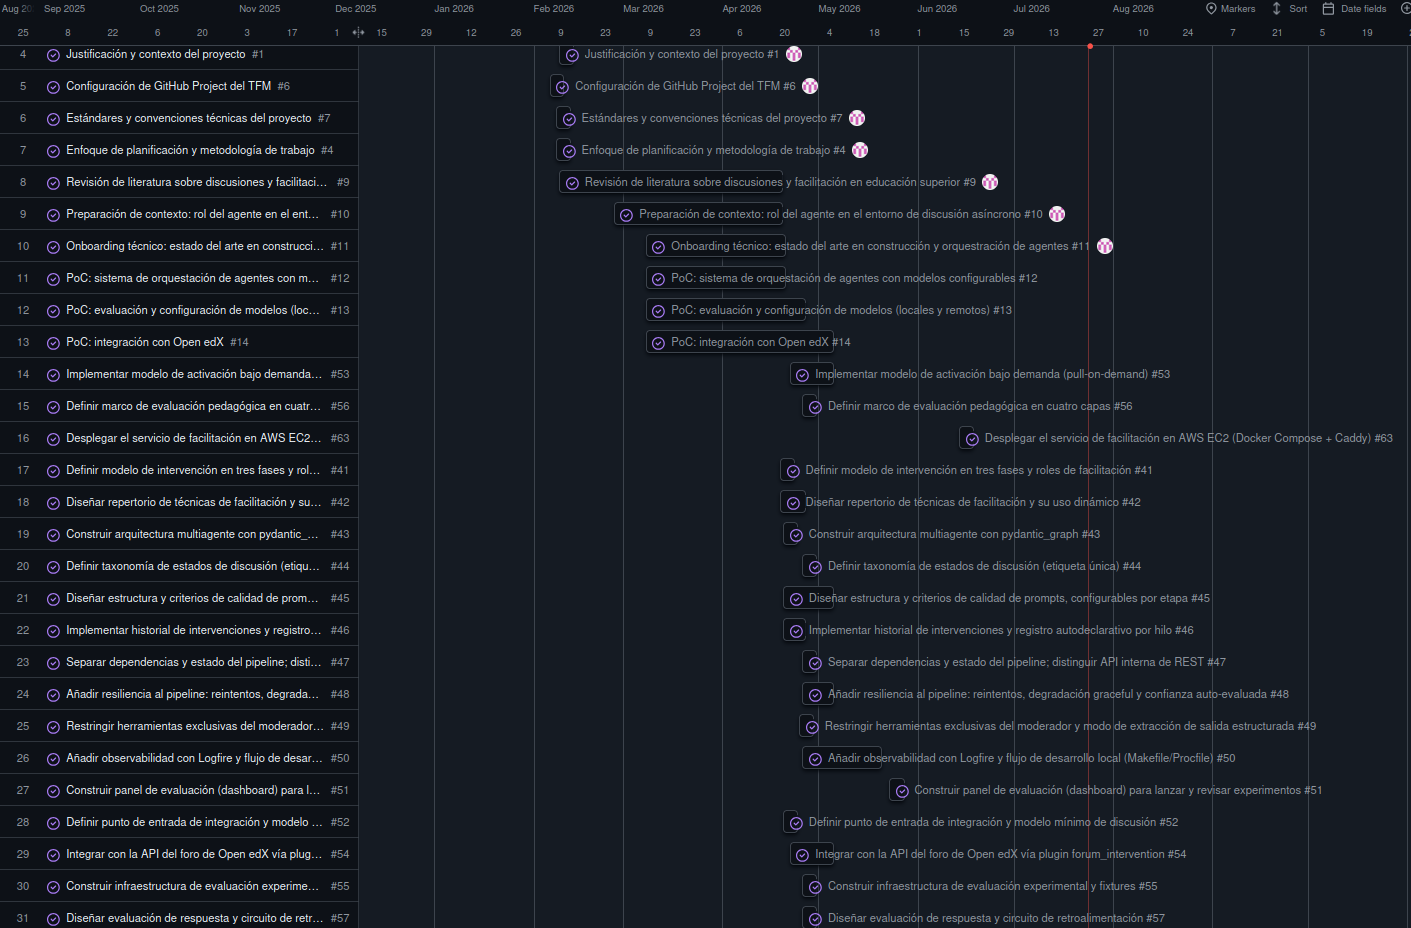
\includegraphics[width=\linewidth]{figures/roadmap-github-project.png}
\caption{Cronología del proyecto registrada en GitHub Project. Cada barra corresponde a una tarea vinculada con su issue; la vista refleja tanto la secuencia como el solapamiento del trabajo de investigación, implementación, integración y evaluación.}
\label{fig:roadmap-github-project}
\end{figure}
\end{landscape}

\section{Preguntas de investigación}

La investigación comenzó con preguntas exploratorias, antes de tomar ninguna decisión de diseño. El punto de partida fue la observación de que las discusiones asíncronas en plataformas educativas no producen el tipo de aprendizaje que sí ocurre en un aula presencial, y que no estaba claro por qué ni qué se podría hacer al respecto.

\subsection{Fase exploratoria}

Las primeras preguntas apuntaban a entender esa dinámica:

\begin{itemize}
  \item ¿Qué ocurre en un aula presencial que no ocurre en una discusión asíncrona? ¿Por qué la dinámica social del aprendizaje no se traslada a los foros de texto?
  \item ¿Qué hace a un facilitador efectivo? ¿Qué acciones concretas produce un instructor cuando interviene en una discusión?
  \item ¿Cómo se ve el proceso de intervención desde dentro? ¿Qué información necesita un facilitador para tomar una decisión?
  \item ¿Es posible hacer ese proceso observable y controlable, o es opaco por naturaleza?
\end{itemize}

Estas preguntas guiaron la revisión de la literatura y la exploración técnica inicial. La respuesta a la cuarta pregunta, en particular, determinó la dirección del diseño, puesto que si el proceso de intervención puede describirse como un conjunto de condiciones observables más una acción correspondiente, puede implementarse como un pipeline; si no puede, la automatización no es viable. La evidencia de los sistemas de tutoría inteligente \parencite{VanLehn2011} y la literatura sobre roles de facilitación \parencite{PilkingtonWalker2003} sugirió que sí es posible, dentro de límites.

\subsection{Fase de diseño}

Una vez delimitado el problema, las preguntas se volvieron más concretas:

\begin{itemize}
  \item ¿Cómo pueden operacionalizarse los roles de facilitación como agentes LLM en un pipeline de análisis de discusiones?
  \item ¿Qué criterios permiten detectar automáticamente el estado de una discusión para determinar si y cuándo intervenir?
  \item ¿Qué criterios permiten evaluar si una intervención generada por IA es pedagógicamente adecuada?
  \item ¿Puede el motor recibir discusiones de una plataforma educativa sin acoplar el pipeline a su modelo de datos?
\end{itemize}

Estas preguntas estructuran el capítulo de desarrollo, ya que cada una corresponde a un componente del sistema o a una decisión de diseño documentada.

\section{Flujo de trabajo}

El proyecto usa un flujo de trabajo de I+D inspirado en prácticas ágiles, con kanban como herramienta de seguimiento pero sin sprints fijos. La incertidumbre propia de la investigación no se ajusta bien a iteraciones de duración predeterminada, algunas preguntas se resuelven en días y otras requieren semanas de exploración antes de poder tomar una decisión.

En la práctica, el trabajo se organiza en ciclos de descubrimiento, de forma que los hallazgos de cada fase informan la siguiente. Las herramientas principales son los issues, el tablero del proyecto y los Architecture Decision Records (ADRs), disponibles en el \href{https://github.com/magrimal/tfm-2026-discussion-moderation}{repositorio del proyecto}. Los \textbf{issues} recogen lo que debe explorarse o implementarse y proporcionan contexto suficiente para retomar el trabajo más adelante. El \textbf{tablero} muestra el estado del trabajo sin fijar sprints artificiales. Los \textbf{ADRs} registran las decisiones de diseño significativas, su razonamiento y las alternativas descartadas, por lo que funcionan como memoria del proyecto. Los \textbf{hitos} delimitan las fases; cada fase termina cuando se responden las preguntas que la definen, no cuando expira un plazo. Se prioriza el enlace al tablero sobre una captura, porque su contenido cambia durante el proyecto y la imagen quedaría desactualizada.

En esta memoria solo se reportan decisiones de diseño respaldadas por evidencia trazable en resultados, tablas, figuras o ADRs del proyecto. Antes de comprometerse con una implementación, cada área de incertidumbre técnica se aborda mediante un spike o prueba de concepto, sin calidad de producción, cuyo objetivo es reducir incertidumbre y documentar hallazgos, no entregar código mantenible.

\subsection{Uso de asistentes de IA en la implementación}

La implementación técnica se realizó con apoyo de asistentes de programación basados en LLM, en particular Claude y Codex. Se usaron para generar borradores de código y documentación, explorar alternativas, localizar inconsistencias y proponer pruebas. El trabajo siguió un ciclo iterativo de propuesta, revisión, prueba y corrección.

La autora definió el problema, aceptó o rechazó las propuestas y asumió la responsabilidad sobre las decisiones, los experimentos y el texto final. No se calculó un porcentaje de código humano o generado por IA, los cambios pasaron por varias iteraciones y el historial de Git no permite atribuir de forma fiable cada línea a una única fuente.

\section{Estructura del documento}

El documento se organiza en siete capítulos. El capítulo~\ref{chap:introduccion} presenta el problema, delimita el alcance y recoge los objetivos, las preguntas de investigación y el plan de trabajo; el capítulo~\ref{chap:introduction-en} ofrece su versión en inglés. El capítulo~\ref{chap:estado-arte} revisa la literatura sobre facilitación y los sistemas de IA que abordan partes del problema. El capítulo~\ref{chap:desarrollo} presenta la experiencia de uso del panel y explica el pipeline, sus decisiones de intervención, las fuentes de datos y los entornos de despliegue. El capítulo~\ref{chap:resultados} documenta los experimentos y las intervenciones generadas. Por último, el capítulo~\ref{chap:conclusiones} recoge las conclusiones, las limitaciones y el trabajo futuro, y el capítulo~\ref{chap:conclusions-en} presenta su versión en inglés.

\chapter{Introduction}
\label{chap:introduction-en}

This chapter situates the difficulties involved in sustaining the facilitation of asynchronous academic discussions when participation grows or the instructor must attend to several threads during the same period. It then sets out the objectives and research questions, describes the work plan and workflow, and closes with the document structure.

\section{Context}

According to social constructivism, learning happens through interaction, in which students construct knowledge by discussing meaning with other students \parencite{WooReeves2007}. In higher education, debates are one of the techniques that best exploit this dynamic because they increase critical thinking and collaborative learning \parencite{Brown2015}, give quieter students a voice, and create a more equitable space for participation than a purely lecture-based class \parencite{BineyEkeyi2018,WooReeves2007}. These discussions may take place in the classroom, where an instructor guides the exchange in real time, or outside it through digital platforms. Outside the classroom, the work is usually asynchronous, so participants contribute at different times without needing to be in the same place.

The digital platforms that support this asynchronous work have grown significantly in Europe in recent years. In 2021, 100\% of institutions in the European Higher Education Area already used some form of digital learning \parencite{GaebelEtAl2021}. A survey published that year found that blended learning was used in 75\% of institutions and that 36\% offered at least one fully online degree program \parencite{GaebelEtAl2021}. These platforms are known as learning management systems (LMSs) and, depending on the institution, may provide the main course environment or complement in-person education. Moodle, Canvas, Open edX, and Coursera, for example, allow content, activities, and discussion forums to be organized in a single environment, with instructor-led or self-paced courses.

The 2020 pandemic accelerated the adoption of digital learning. During the first four months of the crisis, several institutions reported more progress in digitalization than in the four previous years \parencite{GaebelEtAl2021}. Consequently, interaction between students came to happen almost exclusively through digital tools, and discussion forums became one of its main mechanisms in online education \parencite{Rovai2007,MasseyEtAl2019}.

In this context, discussion forums offer forms of participation that are difficult to sustain in an in-person classroom, including scale, turn-taking equity, and scheduling flexibility. A study of 5,104 students in parallel discussions through Moodle illustrates the volume of participants that can be brought together in this type of environment \parencite{ZulfikarEtAl2019}. They also give each student more opportunities to participate than the in-person format, where the instructor can take approximately 65\% of talk time \parencite{SullivanPratt1996}, since everyone can contribute regardless of location or schedule availability \parencite{MasseyEtAl2019}. Forums also support forms of assessment based on the quality of contributions, which can measure critical thinking more directly than a traditional exam \parencite{HoSwan2007,Rovai2007}.

These possibilities have extended the use of forums across settings of very different scales, including massive open online courses (MOOCs). As the number of participants and active discussion threads grows, so does the work required to facilitate the discussions. This difficulty provides the starting point for the next section.

\section{Motivation}

The facilitation of asynchronous discussions falls mainly on the instructor, who performs organizational, intellectual, and social functions, according to Paulsen's classification as reported by Abdous \parencite{Abdous2011}. In one study, 79.3\% of contributions reached deep critical thinking \parencite{LimEtAl2011}. In another, structured roles increased knowledge construction in the groups studied, particularly at the beginning of the discussions \parencite{DeWeverEtAl2010}. Rovai proposes 20--30 students as a practical estimate for an active discussion forum and warns that a larger number may overburden facilitation \parencite{Rovai2007}. In postgraduate courses, 57\% of the recorded instructor-presence behaviors corresponded to social presence \parencite{RichardsonEtAl2015}; corrective feedback represented only 4.9\% of posts in another study \parencite{BlignautTrollip2003}; and facilitators reported difficulty preserving depth across concurrent discussions \parencite{Mansour2024}. The problem becomes more acute in MOOCs, where a single course may include thousands of students \parencite{GuEtAl2021,YuEtAl2024maic}.

Available reviews document that these applications concentrate mainly on personalized tutoring, feedback generation, and curriculum design assistance \parencite{ChuEtAl2025}. However, the facilitation of group discussions remains less explored. Existing natural language processing (NLP) work concentrates on classification tasks, such as toxicity detection; the production of interventions intended to improve discussion quality receives less attention \parencite{KorreEtAl2025}. These reviews more often describe uses aimed at structuring learning conditions than active interventions in group dynamics \parencite{CasebourneEtAl2025}. Some work addresses discussion facilitation directly, including a case-based reasoning system for generating suggestions in online forums \parencite{GuEtAl2021}, and MAIC (\textit{Massive AI-empowered Course}), which organizes teaching functions in massive environments using multiple LLM agents \parencite{YuEtAl2024maic}.

Facilitation requires deciding when a discussion needs support, what type of intervention may be appropriate, and how to formulate it. This work addresses that need with a system that analyzes asynchronous academic discussion threads and proposes interventions based on facilitation criteria.

\section{Objectives}

The objective is to design and implement a system based on LLMs and context engineering techniques to analyze and facilitate asynchronous, text-based academic discussions from different sources. The system uses thread content and criteria derived from the pedagogical literature to decide whether to intervene and to produce a contextualized response.

The specific objectives are the following:

\begin{itemize}
  \item Design and implement an LLM-based agent system, organized in stages, capable of producing interventions coherent with the discussion topic and with conversational continuity, within reasonable time and resource consumption.
  \item Define and implement a context engineering strategy grounded in the literature that organizes thread content, facilitation roles, and techniques, using performance criteria derived from how an instructor effectively facilitates a discussion.
  \item Define a common input contract and use it with reproducible scenarios, six anonymized historical threads preserved in the repository, and a proof of concept with Open edX as a source.
  \item Evaluate the system's behavior in scenarios derived from the literature and in imported threads, examining the classifications produced and the estimated adequacy of the generated interventions.
\end{itemize}

\section{Work plan}

The work partially follows the \textit{Design Science Research} process of \textcite{PeffersEtAl2007}.

The project uses six milestones (table~\ref{tab:milestones-en}) covering problem exploration, design and implementation, inputs and outputs, technical evaluation, and deployment.

\begin{table}[h]
\centering
\small
\renewcommand{\arraystretch}{1.15}
\begin{tabularx}{\textwidth}{@{}Z{3.8cm}Y@{}}
\toprule
\textbf{Milestone} & \textbf{Description} \\
\midrule
1. Problem definition & Formalization of the problem, objectives, requirements, and methodological approach. \\
2. Research and exploration & Proof-of-concept tests to reduce technical uncertainty before design. \\
3. Implementation & Design and implementation of the system based on the findings from the previous milestone. \\
4. Inputs and outputs & Common input contract, execution result, and proof of concept with Open edX. \\
5. Quality assurance and feedback & Evaluation, result collection, and preparation of the final documentation. \\
6. Deployment and infrastructure & Operation of the environments used for the experiments and technical demonstration. \\
\bottomrule
\end{tabularx}
\caption{Project milestones and their relationship to the research, implementation, and evaluation phases.}
\label{tab:milestones-en}
\end{table}

Figure~\ref{fig:roadmap-github-project} provides the corresponding timeline recorded in GitHub Project and shows where the research, implementation, integration, and evaluation tasks overlapped.

\section{Research questions}

The research began with exploratory questions before any design decisions were made. The initial hypothesis was that asynchronous discussions on educational platforms might not produce the same type of learning as an in-person discussion. It was not yet clear what could explain this difference or how it might be addressed.

\subsection{Exploratory phase}

The first questions aimed to understand that dynamic:

\begin{itemize}
  \item What happens in an in-person classroom that does not happen in an asynchronous discussion? Why doesn't the social dynamic of learning carry over to text forums?
  \item What makes a facilitator effective? What concrete actions does an instructor perform when intervening in a discussion?
  \item What does the intervention process look like from the inside? What information does a facilitator need to make a decision?
  \item Can the intervention process be described through observable and controllable decisions?
\end{itemize}

These questions guided the literature review and the initial technical exploration. The fourth question had a particular influence on the design. Evidence from intelligent tutoring systems \parencite{VanLehn2011} and the literature on facilitation roles \parencite{PilkingtonWalker2003} support framing the intervention process as a sequence of steps with recordable intermediate decisions.

The state-of-the-art review in Chapter~\ref{chap:estado-arte} examines the instructor functions and facilitation roles described in the literature. On this basis, the design questions focused on how to represent those functions in the system.

\subsection{Design phase}

Once the problem was delimited, the questions became more concrete:

\begin{itemize}
  \item How can facilitation roles be operationalized as LLM agents in a discussion analysis sequence?
  \item What criteria allow automatic detection of a discussion's state to determine whether and when to intervene?
  \item What criteria allow evaluation of whether an AI-generated intervention is pedagogically appropriate?
  \item Can the system receive discussions from an educational platform without coupling the sequence to its data model?
\end{itemize}

These questions structure the development chapter, since each one corresponds to a system component or a documented design decision.

\section{Workflow}

The project uses an R\&D workflow inspired by agile practices, with kanban as the tracking tool but without fixed-length iterations. Some questions are resolved in days, whereas others require weeks of exploration before a decision can be made.

In practice, the work is organized in discovery cycles, so the findings from each phase inform the next. Tasks, the GitHub board, and Architecture Decision Records (ADRs), available in the project repository\footnote{\href{https://github.com/magrimal/tfm-2026-discussion-moderation}{Project repository}; \href{https://github.com/users/magrimal/projects/3/views/1}{work board}}, document the exploration and design decisions. Milestones delimit the phases, and each phase ends when the questions that define it have been answered.

Technical uncertainties are examined through exploratory tests or proof-of-concept implementations before design decisions are consolidated. These tests have a limited scope and guide subsequent development.

\subsection{Use of AI assistants}

The implementation was carried out with support from LLM-based programming assistants, in particular Claude Code and Codex. They were used to draft code and documentation, explore alternatives, locate inconsistencies, and propose tests. NotebookLM and Google Scholar Labs were used to explore terminology and locate literature. Grammarly and ChatGPT supported grammatical review and iterative improvement of drafts. The work followed cycles of proposal, review, testing, and correction.

The problem was defined and proposals were accepted or rejected; responsibility for decisions, experiments, and the final text was retained throughout. No percentage of human- versus AI-authored code was calculated; Git history documents the implementation process in enough detail to reconstruct it.

\section{Document structure}

This document is organized into seven chapters, including the required English versions of the introduction and conclusions. Chapter~\ref{chap:introduccion} presents the problem, objectives, research questions, and work plan in Spanish, and this chapter provides its English version. Chapter~\ref{chap:estado-arte} reviews discussion facilitation and related educational systems. Chapter~\ref{chap:desarrollo} describes the architecture, facilitation model, analysis sequence, inputs and outputs, context strategy, inspection panel, and deployment environments. Chapter~\ref{chap:resultados} reports the experiments. Finally, Chapter~\ref{chap:conclusiones} presents the conclusions, limitations, and future work in Spanish, and Chapter~\ref{chap:conclusions-en} provides the corresponding English version. Appendix~\ref{app:flujo-prototipo} preserves the complete interface usage sequence.

\chapter{Estado del Arte}
\label{chap:estado-arte}

Este capítulo desarrolla la base conceptual necesaria para abordar las preguntas de investigación de la sección~\ref{sec:preguntas-investigacion}. La primera parte examina la discusión como proceso de aprendizaje, las funciones que desempeña el instructor al facilitarla y la información disponible cuando el intercambio ocurre por escrito y en momentos distintos. La segunda estudia cómo los sistemas inteligentes en educación han representado algunas de esas funciones, desde los agentes pedagógicos hasta los sistemas basados en modelos de lenguaje de gran escala y las arquitecturas multiagente.

\section{Facilitación de discusiones académicas}

\subsection{La discusión como proceso de aprendizaje}

La primera pregunta de la fase exploratoria plantea qué diferencia una discusión académica de otras formas de aprendizaje. La literatura la describe como un proceso de construcción conjunta en el que los participantes formulan ideas, las contrastan y las revisan a partir de las aportaciones del grupo \parencite{Murphy2018,Mercer2000,Glina2012}. Su valor aparece cuando una contribución retoma, cuestiona o amplía otra, ya que esta relación entre aportaciones permite observar el razonamiento del grupo y ofrece oportunidades de participación distintas de las de una clase expositiva.

Para diseñar el sistema era necesario pasar de esa descripción general a decisiones observables: qué señales lee un instructor, cuándo espera y qué acción realiza si decide intervenir.

\subsection{El rol del instructor en la facilitación}

La segunda pregunta examina qué hace el instructor cuando facilita una discusión. La literatura muestra que lee el hilo de discusión, interpreta si los participantes exploran, integran ideas o llegan a conclusiones, y decide si conviene intervenir o esperar \parencite{Abdous2011,Rovai2007,GarrisonEtAl2000}. Cuando interviene, la literatura distingue de forma recurrente funciones organizacionales, intelectuales y sociales \parencite{Paulsen1995,Abdous2011,BlignautTrollip2003}. Estas funciones proporcionan la base de los roles utilizados por el sistema:

\begin{itemize}
    \item \textbf{Rol organizacional}: gestiona la estructura de la discusión, las normas de participación y la continuidad del hilo de discusión \parencite{Paulsen1995,Abdous2011,PilkingtonWalker2003}.
    \item \textbf{Rol intelectual}: formula preguntas, conecta argumentos y orienta el razonamiento del grupo \parencite{Abdous2011,Murphy2018,PilkingtonWalker2003}.
    \item \textbf{Rol social}: favorece la participación y la relación entre las contribuciones de los estudiantes \parencite{Paulsen1995,Abdous2011,BlignautTrollip2003}.
    \item \textbf{Rol afectivo}: reúne acciones de motivación, reconocimiento y apoyo emocional documentadas en los agentes pedagógicos \parencite{SikstromEtAl2022}.
    \item \textbf{Rol moderador}: identifica contenido problemático y contempla su escalado para revisión \parencite{Rovai2007,KorreEtAl2025}.
\end{itemize}

Los tres primeros roles trasladan categorías recurrentes de la literatura. Durante el diseño, las funciones afectivas y de moderación se separaron en dos roles operativos porque requieren instrucciones y herramientas diferentes. Esta separación constituye una decisión de implementación cuya utilidad pedagógica todavía no se ha validado.

\subsection{Discusiones asíncronas y comunicación mediada}

La comunicación mediada por computador comprende los intercambios que se desarrollan mediante sistemas digitales. Dentro de esta categoría, este trabajo se centra en discusiones escritas y asíncronas, en las que los participantes intervienen en momentos distintos \parencite{Rovai2007,MasseyEtAl2019}. La tercera pregunta de la fase exploratoria examina qué información puede utilizar el facilitador en estas condiciones. La asincronía ofrece tiempo para elaborar una respuesta y permite participar sin coincidir en horario, pero elimina señales inmediatas de comprensión, desacuerdo o retirada. El instructor tiene que reconstruir la trayectoria a partir del texto, las relaciones entre mensajes y el tiempo transcurrido. La ausencia de una respuesta puede indicar reflexión, desconexión o cierre; el volumen de mensajes tampoco garantiza avance conceptual \parencite{Rovai2007,MasseyEtAl2019}.

Esta ambigüedad se combina con un problema de atención. Cada hilo conserva su historial, pero el instructor debe seguir muchos intercambios en paralelo y decidir cuáles requieren presencia. La dificultad aumenta en cursos masivos, donde el volumen de participantes hace más costoso sostener una facilitación continua \parencite{GuEtAl2021,YuEtAl2024maic}. Por eso, el problema técnico comprende la interpretación de la trayectoria del hilo de discusión, la decisión de actuar y, cuando corresponde, la generación de una respuesta.

\section{Sistemas inteligentes en educación}

Esta sección examina los sistemas inteligentes en educación para identificar conceptos y patrones de diseño relacionados con el sistema propuesto. Primero se presentan los agentes pedagógicos y los sistemas de tutoría inteligente. Después se estudian los agentes basados en modelos de lenguaje de gran escala, los sistemas multiagente y las aplicaciones desplegadas a mayor escala. Cuando los trabajos revisados incluyen una evaluación, se describe únicamente la evidencia necesaria para interpretar su relación con este trabajo.

\subsection{Agentes pedagógicos y comunicativos}

Los agentes pedagógicos son sistemas de software que se comunican con estudiantes en entornos de aprendizaje digital. El marco de referencia más empleado para evaluarlos es la Comunidad de Indagación \parencite{GarrisonEtAl2000}, que organiza el aprendizaje en línea en torno a tres presencias. La presencia cognitiva abarca la construcción de conocimiento; la social, la proyección de identidad y la cohesión grupal; y la docente, el diseño y la facilitación. Las funciones comunicativas documentadas en estos agentes se dividen en procesos intrapersonales (motivación, autorregulación), andamiaje interpersonal (retroalimentación, pistas) y facilitación de la colaboración grupal \parencite{SikstromEtAl2022}. Los sistemas actuales son efectivos en los dos primeros tipos de función, pero aún carecen de capacidad para sostener conversaciones recíprocas fluidas a nivel de grupo \parencite{SikstromEtAl2022}. La evidencia reciente muestra que las arquitecturas con múltiples agentes y roles diferenciados (tutor, par, agente enseñable) producen beneficios pedagógicos que los sistemas de un solo agente no logran \parencite{LippertEtAl2020}, lo que sugiere que la diferenciación de roles es una vía para resolver esa brecha.

En el contexto específico de las discusiones mediadas por computador, la investigación ha documentado qué roles de facilitación sostienen conversaciones productivas. Los roles de gestión permiten mantener el foco, gestionar tiempos y subtareas; los de construcción de comunidad establecen normas de participación y crean un espacio donde compartir ideas sin riesgo; y los de argumentación consisten en formular, cuestionar y contracuestionar razonamientos con justificación explícita \parencite{PilkingtonWalker2003}. La síntesis de \textcite{Abdous2011} organiza las funciones del facilitador en categorías intelectual, social y de gestión, e incluye el resumen de las contribuciones entre las habilidades relevantes para sostener la discusión. Estas acciones de gestión, construcción de comunidad y argumentación proporcionan antecedentes concretos para definir las intervenciones que genera el sistema según el estado de la discusión.

La forma más estudiada de agente pedagógico adaptativo es el sistema de tutoría inteligente (ITS). Una revisión de 85 estudios muestra que los ITS producen un tamaño del efecto de $d \approx 0{,}76$ (d de Cohen, que mide la diferencia entre grupos en unidades de desviación típica; 0,76 indica una mejora sustancial) respecto a la instrucción en clase, comparable al de la tutoría humana, con sistemas como AutoTutor y Cognitive Tutor de Carnegie Learning como referentes empíricos \parencite{VanLehn2011}. Los sistemas más avanzados alcanzan fiabilidad comparable a la de evaluadores humanos en el rastreo del dominio de contenidos y las características cognitivas de los estudiantes \parencite{GraesserEtAl2017}. Sin embargo, los ITS asumen un modelo de dominio con respuestas correctas e incorrectas, supuesto que no se sostiene en discusiones académicas abiertas donde puede no existir una única respuesta de referencia. La evidencia sobre aprendizaje productivo por fracaso añade una restricción relevante, pues los estudiantes que trabajan un problema sin asistencia antes de recibir instrucción obtienen mejores resultados de transferencia que los que reciben instrucción desde el inicio \parencite{Kapur2016}, lo que indica que intervenir demasiado pronto puede interferir con el aprendizaje.

De esta revisión se extraen dos aportaciones directas para el diseño del sistema. La taxonomía de roles de \textcite{PilkingtonWalker2003} (gestión, construcción de comunidad y argumentación) define los tipos de intervención que el sistema debe producir, y el principio de aprendizaje productivo por fracaso \parencite{Kapur2016} sustenta la regla de no intervenir mientras la dinámica de la discusión no ha alcanzado un punto de bloqueo.

\subsection{Modelos de lenguaje de gran escala y agentes en educación}

Los modelos de lenguaje de gran escala pueden realizar una tarea a partir de instrucciones y ejemplos incluidos en la entrada. \textcite{BrownEtAl2020} evaluaron esta capacidad sin proporcionar ejemplos, con un solo ejemplo y con varios ejemplos, sin actualizar los parámetros del modelo para cada tarea. Esta propiedad permite utilizar un mismo modelo para distintas operaciones lingüísticas mediante cambios en las instrucciones y el contexto que recibe.

El término ingeniería del contexto se ha propuesto para describir el diseño, la estructuración y la gestión del entorno informativo que recibe un agente basado en LLMs \parencite{Vishnyakova2026}. El informe técnico de la Cátedra iDanae (UPM y Management Solutions) lo concreta como la optimización de la cantidad de información introducida en una llamada al modelo y de la forma en que se presenta \parencite{IdanaeUPM2026}.

La capacidad de seguir instrucciones y ejemplos permite utilizar modelos generales en distintas tareas lingüísticas. Al mismo tiempo, sus respuestas pueden contener información no sustentada, sesgos o problemas de privacidad \parencite{ChuEtAl2025}. Por esta razón, el sistema conserva sus salidas como respuestas candidatas que pueden inspeccionarse, y su validez pedagógica queda pendiente de una evaluación posterior.

La aplicación de estos agentes en educación se ha concentrado en tutoría personalizada y diseño curricular, con escasa evidencia sobre facilitación de discusiones grupales. Las revisiones sistemáticas disponibles muestran que estas aplicaciones emplean memoria, planificación y herramientas \parencite{ChuEtAl2025}, pero la mayoría se sitúa en niveles intermedios de madurez tecnológica (TRL, \textit{Technology Readiness Level}, 4-6) y la evidencia longitudinal sobre su impacto en el aprendizaje sigue siendo limitada \parencite{KostopoulosEtAl2025}. Alrededor del 70\% de los estudios asignan a la IA la función de estructurar condiciones previas de aprendizaje, mientras que la facilitación activa de la dinámica del grupo aparece con menor frecuencia \parencite{CasebourneEtAl2025}.

Entre los trabajos sobre facilitación activa, \textcite{ChenEtAl2023tutoring} organizan la tutoría adaptativa en tres procesos encadenados de interacción, reflexión y reacción. Otro antecedente es el tutor socrático basado en LLM estudiado por \textcite{DegenAsanov2025}, que aplica la taxonomía de preguntas de \textcite{Paul1990}. En un estudio con 65 estudiantes, este tutor ofreció mayor apoyo al pensamiento crítico que los métodos comparados. En conjunto, ambos trabajos muestran formas de distribuir una intervención educativa entre procesos o responsabilidades diferenciadas, por lo que constituyen antecedentes para la arquitectura que se presenta en el capítulo siguiente.

\subsection{Intervenciones en discusiones académicas}

La investigación sobre intervenciones automatizadas en discusiones complementa ese trabajo orientado a agentes al analizar directamente el problema de cuándo actuar, qué producir y a quién dirigirse.

La investigación en esta área muestra que la generación de intervenciones es técnicamente viable, y que el quién y el cuándo son tan determinantes como el qué. El trabajo existente se ha centrado principalmente en tareas de clasificación, como la detección de toxicidad y el análisis de postura; la producción de intervenciones destinadas a mejorar la calidad de la discusión recibe menos atención \parencite{KorreEtAl2025}. Los estudios de revisión sobre moderación asistida por IA también muestran que el campo se concentra en técnicas restrictivas, como la eliminación de contenido, con escasa exploración de los impactos a nivel grupal \parencite{YuEtAl2024review}. Sobre el cuándo, la evidencia muestra que el descarrilamiento conversacional puede predecirse antes de que ocurra siguiendo la trayectoria del tono a lo largo del hilo \parencite{ChangDanescu2019}. Sobre el qué, hay evidencia de que la generación automatizada de sugerencias de facilitación es factible, con una precisión de 0,679 y una exhaustividad (\textit{recall}) de 0,699 sobre 1.600 publicaciones reales, aunque la verificación humana sigue siendo necesaria para tareas complejas \parencite{GuEtAl2021}. Sobre el quién, un chatbot moderador en discusiones deliberativas (n=64) muestra que dirigirse específicamente a participantes reticentes produce mayor alineación de opiniones, distribución más equitativa de contribuciones y mayor cohesión grupal que intervenir sobre el hilo en general \parencite{KimEtAl2021}.

Estas tres líneas de evidencia informan directamente el diseño del sistema. La predictibilidad del descarrilamiento \parencite{ChangDanescu2019} fundamenta el módulo de clasificación de estados de la discusión, la viabilidad de la generación automatizada \parencite{GuEtAl2021} respalda como antecedente el enfoque técnico adoptado, y la efectividad de las intervenciones dirigidas a participantes específicos \parencite{KimEtAl2021} orienta el diseño de las intervenciones de tipo social.

\subsection{Sistemas multiagente en el aula: SimClass y MAIC}

SimClass\footnote{\url{https://github.com/THU-MAIC/SimClass}} y MAIC\footnote{El repositorio actual del proyecto puede consultarse en \url{https://github.com/THU-MAIC/OpenMAIC}.} fueron desarrollados por equipos de la Universidad Tsinghua, comparten varios autores y estudian arquitecturas multiagente aplicadas a la educación. Cada uno examina una situación distinta y ambos permiten estudiar cómo se distribuyen funciones educativas entre agentes especializados.

SimClass estudia si agentes LLM con roles diferenciados pueden reproducir dinámicas sociales emergentes en una simulación de aula. La base arquitectónica son los agentes generativos dotados de flujo de memoria, reflexión y planificación, que producen comportamientos sociales emergentes en entornos de simulación \parencite{ParkEtAl2023}. SimClass aplica este enfoque a un aula virtual donde un agente instructor, un agente asistente y varios agentes estudiante interactúan con personas diferenciadas (Class Clown, Deep Thinker, Note Taker, Inquisitive Mind) \parencite{ZhangEtAl2024simclass}. El sistema se evalúa con el Sistema de Análisis de Interacción de Flanders (FIAS) y el marco de la Comunidad de Indagación; en experimentos con más de 400 estudiantes de posgrado, produjo comportamientos de grupo emergentes (enseñanza colaborativa, acompañamiento emocional, gestión de la disciplina) y los estudiantes reportaron alta presencia e interacción efectiva \parencite{ZhangEtAl2024simclass}. A partir de estos resultados, SimClass aporta evidencia sobre el uso de roles diferenciados y la aparición de dinámicas grupales en un aula simulada. Sin embargo, su unidad de interacción es el aula virtual completa, mientras que este trabajo analiza hilos de discusión asíncronos recuperados de una fuente externa.

MAIC estudia cómo distribuir funciones docentes entre agentes LLM en una plataforma masiva. El sistema opera en tres etapas (Read, transformación de materiales del curso; Teach, generación de guiones y acciones de enseñanza; y Learn, interacción en el aula) con cinco roles de agente (Teacher, Companion, Assistant, Analyzer y Manager) \parencite{YuEtAl2024maic}. En experimentos con más de 500 estudiantes y más de 100.000 registros de aprendizaje en la Universidad Tsinghua, los autores identifican correlaciones entre la interacción con el sistema y el rendimiento académico. También señalan que los agentes instructores usaban guiones estandarizados para todos los estudiantes y que el impacto observado sobre pensamiento profundo y calidad de la discusión fue limitado \parencite{YuEtAl2024maic}. Por tanto, MAIC resulta relevante para este trabajo por la distribución de funciones docentes entre agentes y por su aplicación a una plataforma educativa masiva. Esa separación de responsabilidades se traslada aquí al análisis y la facilitación de hilos de discusión asíncronos.

\subsection{Plataformas a escala: MOOCs y aplicaciones empresariales}

Más allá de los prototipos de investigación, la aplicación de IA a la facilitación de discusiones educativas también ha generado soluciones comerciales a escala.

Las aplicaciones existentes utilizan modelos de acceso e integración diferentes. Coursera incorporó asistentes basados en GPT-4 en más de 100 cursos, con tiempos de respuesta un 47\% más rápidos que los tutores humanos \parencite{Coursera2024}, mientras que edX reportó 1,2 millones de estudiantes en seis meses utilizando laboratorios virtuales impulsados por IA \parencite{MarketGrowthReports2026}. CONNECT, desarrollado por Human2Human AI, ofrece sesiones de discusión en grupos pequeños moderadas por un facilitador de IA y se integra con LMS compatibles mediante LTI (\textit{Learning Tools Interoperability}) \parencite{Human2Human2025}. Estas aplicaciones muestran distintas formas de incorporar IA a plataformas educativas. El sistema desarrollado en este trabajo se concentra en intervenciones trazables sobre discusiones asíncronas y en un contrato común para recibir los hilos.

\section{Conclusiones del estado del arte}

Los sistemas inteligentes en educación muestran resultados favorables en tutoría individual y permiten simular aulas con múltiples roles, aunque la facilitación de hilos de discusión asíncronos sigue menos explorada. Según \textcite{CasebourneEtAl2025}, alrededor del 70\% de los estudios revisados asignan a la IA la función de estructurar las condiciones de aprendizaje, mientras que su participación activa en una conversación grupal aparece con menor frecuencia. En este contexto, SimClass estudia dinámicas de aula simuladas y MAIC distribuye funciones docentes en una plataforma educativa masiva. Entre los sistemas revisados, ninguno aborda un problema similar al de este trabajo, que consiste en recibir un hilo de discusión procedente de una fuente externa, analizar si necesita apoyo y producir una intervención cuya generación pueda inspeccionarse.

La facilitación automatizada de un hilo asíncrono requiere dos capacidades. La primera es interpretar el hilo para reconocer señales como estancamiento, desvío o conflicto \parencite{WeiEtAl2017,AgrawalEtAl2015,LiuEtAl2015}. La segunda es producir una respuesta contextualizada, como una pregunta de seguimiento, una conexión entre aportaciones o una síntesis \parencite{SengarEtAl2025,KilincKececioglu2024,BrownEtAl2020}. Una única instrucción de entrada (\textit{prompt}) podría reunir ambas tareas, aunque combinaría sus instrucciones y estados y reduciría la independencia de cada etapa y la inspección de las decisiones intermedias. Por esta razón, el diseño las organiza en etapas sucesivas de clasificación, decisión y generación.

El marco de \textcite{DwivediEtAl2026} proporciona conceptos para describir sistemas que combinan planificación, memoria compartida, herramientas y distribución de tareas entre agentes. Estos conceptos se utilizarán en el capítulo siguiente para caracterizar la arquitectura implementada.

La revisión también produjo un repertorio de técnicas y condiciones para decidir cuándo conviene esperar. El inventario de fuentes está disponible en el archivo de revisión bibliográfica del repositorio\footnote{\href{https://github.com/magrimal/tfm-2026-discussion-moderation/blob/main/docs/literature/papers.csv}{Repositorio del proyecto, \texttt{docs/literature/papers.csv}}}, y cada técnica conserva sus referencias. La evidencia sobre fracaso productivo advierte que una ayuda temprana puede interrumpir una dificultad todavía útil en tareas con una solución identificable \parencite{Kapur2016,VanLehn2011}. Su aplicación a discusiones abiertas constituye una hipótesis de diseño que requiere validación posterior.

El capítulo siguiente presenta la arquitectura del sistema y explica cómo organiza la clasificación, la decisión de intervenir y la generación de la respuesta en etapas sucesivas.

\chapter{Diseño e implementación}
\label{chap:desarrollo}

Este capítulo describe el diseño y la implementación del sistema. Primero presenta la arquitectura general y sitúa los componentes que reciben los hilos de discusión, ejecutan el análisis y conservan los resultados. Después explica el modelo de facilitación, las entradas y salidas, y la secuencia interna de decisiones. Las últimas secciones describen la estrategia de contexto, el panel utilizado para ejecutar e inspeccionar los análisis y los entornos de despliegue.

\section{Arquitectura del sistema}
\label{sec:arquitectura-sistema}

La arquitectura distingue las fuentes de hilos de discusión, el servicio que realiza el análisis, el panel, los proveedores de modelos y los mecanismos utilizados para conservar e inspeccionar los resultados.

\subsection{Visión general}

El sistema se organiza alrededor del servicio de facilitación, que recibe un hilo de discusión mediante un formato común y devuelve las decisiones tomadas durante el análisis. Cuando corresponde intervenir, el resultado también incluye una respuesta candidata.

El servicio ofrece una API de Python para las llamadas directas y una API REST para los clientes remotos. De este modo, los scripts experimentales utilizan la API de Python, mientras que el panel se comunica con el servicio mediante la API REST. Además, el servicio utiliza los proveedores de modelos configurados durante el análisis y conserva los resultados y los registros técnicos para su posterior inspección.

La tabla siguiente resume los componentes principales. Las secciones posteriores explican sus contratos, su funcionamiento interno y las implementaciones empleadas durante los experimentos.

\subsection{Componentes principales}

\begin{table}[htbp]
\centering
\small
\renewcommand{\arraystretch}{1.12}
\begin{tabularx}{\textwidth}{@{}Z{3.5cm}Y@{}}
\toprule
\textbf{Componente} & \textbf{Función} \\
\midrule
Fuentes de hilos de discusión & Proporcionan las discusiones mediante el formato común de entrada. \\
Servicio de facilitación & Analiza la discusión y genera una respuesta candidata cuando corresponde. Expone una API de Python y una API REST. \\
Panel & Permite iniciar los análisis e inspeccionar sus resultados mediante la API REST. \\
Proveedores de modelos & Proporcionan los modelos utilizados por el servicio. \\
Almacenamiento y registro técnico & Conservan los resultados y la información necesaria para revisar las ejecuciones. \\
\bottomrule
\end{tabularx}
\caption{Componentes principales del sistema y su función.}
\label{tab:componentes-principales}
\end{table}

\subsection{Estructura de la implementación}

Las decisiones arquitectónicas se registraron durante el desarrollo mediante registros de decisiones de arquitectura (\textit{Architecture Decision Records}, ADRs). Esta sección describe las decisiones necesarias para entender la implementación, mientras que los ADRs conservan su razonamiento técnico y las alternativas consideradas.

El código, la integración con Open edX, los scripts, la documentación y la infraestructura se versionan en un repositorio único. Esta organización permite mantener juntos los componentes utilizados para desarrollar y evaluar el sistema. El servicio de Python se encuentra en \texttt{discussion\_moderation}, el panel en \texttt{dashboard}, la integración con Open edX en \texttt{integrations} y la automatización auxiliar en \texttt{scripts}. La estructura principal, obtenida con \texttt{tree} y reducida para omitir directorios generados y detalles internos, es la siguiente:

\begin{samepage}
\begin{small}
\begin{verbatim}
.
|-- dashboard/                 # Frontend React
|-- discussion_moderation/     # Servicio Python
|   |-- agents/
|   |-- api/
|   |-- evals/
|   |-- graph/
|   |-- rest_api/
|   `-- tools/
|-- docs/
|   |-- decisions/
|   |-- deployment/
|   |-- experiments/
|   |-- literature/
|   |-- thesis/
|   `-- threads/
|-- integrations/
|   `-- openedx/
`-- scripts/
\end{verbatim}
\end{small}
\end{samepage}

Los resultados de cada ejecución se guardan en el sistema de archivos o en S3. Un manifiesto organiza los casos por modelo e hilo de discusión y conserva las decisiones intermedias, la respuesta cuando existe, la duración, los errores y los mensajes necesarios para inspeccionar la ejecución.

\section{Modelo de facilitación}
\label{sec:modelo-facilitacion}

El modelo de facilitación describe las decisiones que realiza el servicio al analizar un hilo de discusión. El proceso se divide en tres etapas:

\begin{enumerate}
  \item \textbf{Analizar la discusión}: se clasifica el estado del hilo de discusión y se decide si la evidencia justifica una intervención.
  \item \textbf{Seleccionar la acción}: cuando corresponde intervenir, se eligen un rol y una técnica de facilitación.
  \item \textbf{Generar la respuesta}: el agente asociado al rol produce una respuesta candidata.
\end{enumerate}

La implementación divide la primera etapa en dos llamadas al LLM, una para la clasificación y otra para la decisión de intervenir. La selección del rol y la generación de la respuesta utilizan otras dos llamadas. Las tres etapas conceptuales se ejecutan, por tanto, mediante cuatro llamadas.

Esta secuencia se representa mediante un grafo dirigido. Cada decisión corresponde a un nodo y los resultados intermedios se transmiten mediante un estado compartido. Las transiciones determinan el siguiente nodo y permiten terminar la ejecución cuando se decide que no conviene intervenir.

Las taxonomías de estados, roles y técnicas convierten los conceptos revisados en el estado del arte en valores que los nodos pueden devolver y que después pueden inspeccionarse.

\subsection{Estados de la discusión}

Para describir la situación del hilo de discusión se definieron seis posibles etiquetas principales (tabla~\ref{tab:estados}) \parencite{BlignautTrollip2003,AnEtAl2009}. El esquema obliga al clasificador a devolver exactamente una por ejecución. Sin embargo, las situaciones descritas pueden coincidir. Por ejemplo, un hilo de discusión puede estar estancado y fuera de tema al mismo tiempo. La implementación no declara reglas formales de prioridad y deja que el modelo elija la condición principal en su razonamiento. Esta simplificación facilita inspeccionar la decisión, aunque puede ocultar una condición secundaria.

\begin{table}[h]
\centering
\renewcommand{\arraystretch}{1.12}
\begin{tabularx}{\textwidth}{@{}Z{3cm}Y@{}}
\toprule
\textbf{Estado} & \textbf{Descripción} \\
\midrule
Nueva       & Sin respuestas todavía \\
Activa      & Intercambio en curso entre participantes \\
Estancada   & Sin publicaciones nuevas tras un periodo configurable \\
Conflictiva & Lenguaje agresivo o despectivo entre participantes \\
Convergente & Los participantes están llegando a conclusiones \\
Fuera de tema & La discusión se ha alejado del tema propuesto \\
\bottomrule
\end{tabularx}
\caption{Taxonomía de estados de discusión del sistema de facilitación.}
\label{tab:estados}
\end{table}

La etiqueta \emph{estancada} usa un umbral configurable de inactividad, establecido en 48 horas por defecto. Esta señal temporal determina qué estado puede asignar el clasificador, pero no obliga al sistema a intervenir. A la etapa siguiente se le pide distinguir entre el silencio de participantes que todavía pueden estar reflexionando y un bloqueo que justifica apoyo a partir de la trayectoria y la naturaleza de las últimas contribuciones descritas en el razonamiento del clasificador. El campo estructurado de trayectoria se conserva en el resultado, pero no se propaga por separado a las etapas posteriores. Los trabajos sobre tutoría y fracaso productivo indican que, en tareas con una solución identificable, intervenir antes del punto de bloqueo puede interrumpir un proceso útil de exploración \parencite{VanLehn2011,Kapur2016}. El sistema traslada esa idea como hipótesis de diseño a discusiones abiertas, donde no siempre existe una respuesta correcta a la que converger; su validez queda pendiente de evaluación.

Además del estado principal, el clasificador devuelve cuatro dimensiones. La trayectoria distingue entre participación creciente, estable, en declive o que nunca llegó a comenzar. El balance de participación indica si las contribuciones están distribuidas, dominadas por una o dos voces o centradas en el instructor. La calidad del discurso diferencia aportaciones sustantivas, mixtas o formularias. Por último, la fase de indagación sitúa el hilo de discusión en activación, exploración, integración o resolución. Estos criterios se describen de forma cualitativa en el prompt y dependen de la interpretación del modelo.

\subsection{Decisión de intervención}

Después de clasificar el hilo de discusión, una etapa separada decide si la evidencia justifica intervenir. Si la respuesta es negativa, la ejecución termina y conserva la clasificación y la decisión. Si es positiva, la secuencia continúa con la selección del rol y la generación de una respuesta candidata. Esta separación evita que la generación de un texto presuponga que intervenir era necesario.

Cada uno de los cuatro tipos de salida (clasificación, decisión de intervención, selección de rol y respuesta) incluye un campo de confianza auto-evaluada por el modelo, con valor por defecto 1.0. El campo se conserva como instrumentación experimental y no tiene efecto operativo. En los experimentos de este trabajo no se analizó su calibración frente a la exactitud observada, por lo que no se interpreta como una medida fiable de calidad.

\subsection{Roles, técnicas y escalado}

Cuando la decisión de intervención es positiva, la etapa siguiente selecciona el tipo de facilitación que necesita el hilo de discusión. El sistema implementa cinco roles, cada uno representado por un agente con instrucciones y restricciones específicas.

Los roles organizacional, intelectual y social proceden de las categorías revisadas en el estado del arte \parencite{Paulsen1995,Abdous2011,BlignautTrollip2003,DeWeverEtAl2010}. Durante el diseño se separaron otras dos responsabilidades. El rol afectivo reúne las acciones de reconocimiento y apoyo emocional, que utilizan disparadores e instrucciones propios. Por su parte, el moderador se ocupa del marcado y el escalado de situaciones que requieren herramientas restringidas o juicio humano. Esta separación dio lugar a los cinco roles implementados.

La selección del rol corresponde a un agente denominado orquestador. Este agente recibe la clasificación y la decisión de intervenir, y elige uno de los cinco roles. El estado de la discusión orienta la elección, aunque no aplica un filtro determinista. Después, el repertorio completo de técnicas se expone al agente elegido en un mismo orden, también sin filtrar por rol ni por estado. Las categorías anteriores orientan la selección mediante la persona y las restricciones de cada agente, pero no limitan técnicamente qué opción puede devolver. Esta decisión permite selecciones cruzadas cuando el contexto lo justifica y asume el riesgo de sesgo de posición documentado en la literatura sobre listas largas presentadas a LLMs \parencite{ZhengEtAl2023}.

El repertorio incluye la técnica \texttt{instructor\_escalation} para los casos que requieren juicio humano. El agente genera entonces una nota para el instructor, aunque la implementación no dispone de un canal que la entregue. El rol moderador también puede solicitar el marcado de una publicación mediante la herramienta \texttt{flag\_content}. Ambas funciones se probaron con componentes simulados que reproducían las respuestas del foro. Estas pruebas no incluyeron su uso en un curso real.

\section{Entradas y salidas del sistema}
\label{sec:entradas-salidas}

\subsection{Entrada: contrato común}

Los roles y las técnicas anteriores operan sobre el hilo de discusión que recibe el sistema. Para representar esta entrada, el modelo \texttt{DiscussionThread} reúne los campos de la tabla~\ref{tab:contrato-entrada}. Los objetivos de aprendizaje forman parte del modelo, pero pueden quedar vacíos porque la API de hilos no los proporciona. Cuando están disponibles, los incorpora quien inicia la ejecución. El adaptador de Open edX transforma la respuesta de su API a este formato común, mientras que los escenarios de evaluación construyen directamente la misma entrada.

\begin{table}[htbp]
\centering
\small
\renewcommand{\arraystretch}{1.12}
\begin{tabularx}{\textwidth}{@{}Z{3.2cm}Y@{}}
\toprule
\textbf{Información} & \textbf{Representación en el contrato} \\
\midrule
Identificación & \texttt{id}, \texttt{course\_id} \\
Mensaje inicial & Título, contenido, autor y fecha de creación \\
Respuestas & Comentarios con su autor, contenido, fecha y posibles respuestas anidadas \\
Contexto pedagógico & Objetivos de aprendizaje, cuando están disponibles \\
Estado del hilo de discusión & Tipo, última actividad, cierre y existencia de respuestas respaldadas por el instructor \\
Procedencia experimental & Origen del caso, utilizado en los escenarios sintéticos y los hilos históricos \\
\bottomrule
\end{tabularx}
\caption{Campos del contrato común de entrada implementado por \texttt{DiscussionThread}.}
\label{tab:contrato-entrada}
\end{table}

\subsection{Fuentes versionadas}

Las entradas utilizadas en los experimentos combinan escenarios sintéticos y seis hilos históricos anonimizados cargados desde archivos versionados en el repositorio. Los hilos históricos se extrajeron de \textit{Dataset MOOC Forum edX} \parencite{AlarioHoyos2021Dataset}, que reúne foros de tres MOOC de programación y varias ediciones. La versión citada publica el archivo original, su licencia CC BY 4.0 y su suma de comprobación. El repositorio conserva el procedimiento de extracción, los 480 candidatos resultantes y los seis casos seleccionados, junto con la documentación de la selección manual.

Para desarrollo local, pruebas automatizadas y experimentos, los hilos se cargan desde escenarios definidos en el repositorio. Esto hace reproducibles las entradas y evita depender de una instancia externa durante la comparación de modelos.

\subsection{Adaptador de Open edX}

Además de las fuentes versionadas, el sistema puede recuperar hilos de discusión mediante un adaptador. Open edX se utilizó para comprobar esta vía de entrada porque organiza las discusiones como hilos y admite extensiones mediante complementos. Otras plataformas, como Moodle, Canvas o Discourse, requerirían un adaptador propio, que queda fuera del alcance de este trabajo.

Los experimentos y el panel inician el análisis bajo demanda a partir del identificador del hilo de discusión. Además, la prueba de concepto incluye un complemento de Open edX que detecta la creación de hilos, respuestas y comentarios y envía una tarea asíncrona al servicio de facilitación.

El servicio expone una API de Python y una API REST que reutiliza la misma lógica (figura~\ref{fig:activacion-bajo-demanda}). Las herramientas que ejecutan los casos experimentales utilizan la API de Python y conservan sus resultados, mientras que el panel utiliza la API REST. El adaptador, el complemento y estos puntos de comunicación permiten conectar Open edX con el servicio.

\begin{figure}[htbp]
\centering
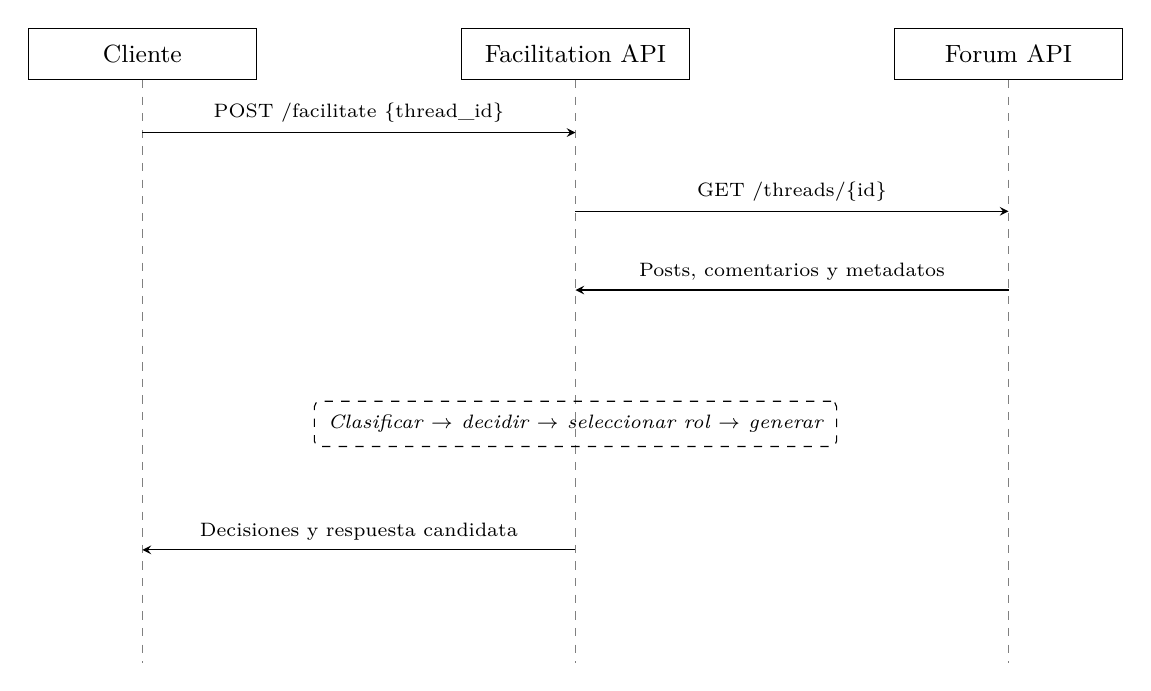
\begin{tikzpicture}[
  head/.style={rectangle, draw, minimum width=2.9cm, minimum height=0.65cm,
               font=\small, text centered},
  life/.style={dashed, gray},
  msg/.style={->, >=stealth, font=\scriptsize},
  box/.style={rectangle, draw, dashed, rounded corners=2pt,
              font=\scriptsize\itshape, align=center, inner sep=5pt}
]

\node[head] (C) at (0,    0) {Cliente};
\node[head] (A) at (5.5,  0) {Facilitation API};
\node[head] (F) at (11,   0) {Forum API};

\draw[life] (C.south) -- ++(0,-7.4);
\draw[life] (A.south) -- ++(0,-7.4);
\draw[life] (F.south) -- ++(0,-7.4);

\draw[msg] (0,-1)     -- (5.5,-1)
    node[midway, above] {POST /facilitate \{thread\_id\}};
\draw[msg] (5.5,-2)   -- (11,-2)
    node[midway, above] {GET /threads/\{id\}};
\draw[msg] (11,-3)    -- (5.5,-3)
    node[midway, above] {Posts, comentarios y metadatos};

\node[box] at (5.5,-4.7) {Clasificar $\rightarrow$ decidir $\rightarrow$ seleccionar rol $\rightarrow$ generar};

\draw[msg] (5.5,-6.3) -- (0,-6.3)
    node[midway, above] {Decisiones y respuesta candidata};

\end{tikzpicture}
\caption{Interacción con Open edX como fuente en la prueba de concepto. El servicio recupera el contenido del hilo de discusión y devuelve las decisiones y, cuando corresponde, una respuesta candidata. Esta ejecución experimental termina al devolver el resultado.}
\label{fig:activacion-bajo-demanda}
\end{figure}

La prueba de concepto incluye también una función opcional de publicación, probada con componentes simulados que reproducían las respuestas del foro. Esta función carece de una revisión previa por parte del profesor. Tampoco consulta \texttt{post\_to\_thread}, el indicador que distingue las respuestas propuestas para el hilo de discusión de las notas dirigidas al instructor. En conjunto, la implementación permite recuperar y adaptar hilos de discusión, iniciar el análisis mediante eventos y comunicar el resultado a Open edX. Quedan pendientes la integración en el uso cotidiano del LMS y la validación de un proceso seguro de revisión y publicación en un curso real.

\subsection{Salida de una ejecución}

Una ejecución comienza con un hilo construido desde una fuente versionada o recuperado mediante el adaptador de Open edX. El panel inicia las ejecuciones a través de la API REST, mientras que las herramientas experimentales llaman a la API de Python. En ambos casos, la secuencia devuelve un \texttt{PipelineResult} con los campos de la tabla~\ref{tab:contrato-salida}. Los resultados posteriores a la clasificación pueden faltar si el sistema decide no intervenir o si una etapa termina con error.

\begin{table}[htbp]
\centering
\small
\renewcommand{\arraystretch}{1.12}
\begin{tabularx}{\textwidth}{@{}Z{3.2cm}Y@{}}
\toprule
\textbf{Parte de la salida} & \textbf{Información conservada} \\
\midrule
Clasificación & Estado principal, trayectoria, balance de participación, calidad del discurso, fase de indagación, razonamiento y confianza declarada \\
Decisión & Indicador de intervención, razonamiento y confianza declarada \\
Selección de rol & Rol elegido, razonamiento y confianza declarada, cuando se decide intervenir \\
Respuesta candidata & Texto, técnica, categoría de acción, razonamiento, confianza declarada y \texttt{post\_to\_thread} \\
Diagnóstico & Mensajes de los agentes y error, cuando se produce; las herramientas experimentales añaden duración y datos del caso al registro persistido \\
\bottomrule
\end{tabularx}
\caption{Contenido del resultado devuelto por la secuencia de facilitación.}
\label{tab:contrato-salida}
\end{table}

El estado compartido acumula estas decisiones durante la ejecución. El indicador \texttt{post\_to\_thread} expresa si una respuesta se propone para el hilo de discusión o para el instructor.

\subsection{Almacenamiento y consulta de resultados}
\label{sec:almacenamiento-resultados}

Los resultados se almacenan en Amazon S3, el servicio de almacenamiento de objetos de AWS. Cada serie de ejecuciones conserva un archivo \texttt{run\_manifest.json} con su estado, el número de casos completados y los resultados agrupados por modelo e hilo de discusión. Para cada caso se registran la clasificación, la decisión de intervención, la respuesta generada cuando existe, la duración y el posible error.

El siguiente extracto abreviado procede de la serie de ejecuciones realizada en Idril. Se han omitido campos para mostrar la organización general del archivo.

\begin{small}
\begin{verbatim}
{
  "run_id": "2026-07-23T11-51-18-threads-4-models",
  "status": "completed",
  "total_runs": 72,
  "completed_runs": 66,
  "error_count": 6,
  "models": {
    "ollama:ministral-3:14b": {
      "threads": {
        "new": {
          "classification": {"state": "new"},
          "intervention": {"decision": "no_intervention"},
          "response": null,
          "duration_ms": 28130,
          "error": null
        }
      }
    }
  }
}
\end{verbatim}
\end{small}

La API lee y valida estos archivos, y el panel solicita mediante ella el resumen y el detalle de cada ejecución. Además, cuando está habilitado, Logfire\footnote{\url{https://logfire.pydantic.dev/docs/}} registra las llamadas, la duración y los errores de la ejecución.

\section{Implementación de la secuencia de análisis y facilitación}
\label{sec:pipeline}

\subsection{Nodos y enrutamiento}

El modelo de facilitación se implementa como un grafo dirigido que ejecuta las decisiones descritas en la sección anterior. Cada etapa corresponde a un nodo con entradas y salidas definidas, y sus resultados se transmiten mediante un estado compartido. El agente asociado al rol consulta el repertorio de técnicas antes de generar el texto.

La separación entre el orquestador y los agentes especializados permite inspeccionar cada etapa, modificar el comportamiento de un rol sin afectar la clasificación y revisar su lógica por separado. Esta organización sigue el patrón de los sistemas de tutoría multiagente \parencite{LippertEtAl2020}. Si la discusión progresa sin apoyo, la secuencia termina después de la decisión de intervención y conserva los resultados producidos hasta ese punto.

La figura~\ref{fig:pipeline} representa las etapas de la implementación. Cuatro de ellas llaman a un modelo:

\begin{itemize}
    \item \texttt{ClassificationNode} caracteriza el hilo de discusión y le asigna un estado de la tabla~\ref{tab:estados}. Cuando la evaluación de clasificación está activa, comprueba después que el razonamiento no esté vacío.
    \item \texttt{InterventionNode} llama al modelo para decidir si la evidencia justifica intervenir. La comprobación de esta etapa determina el siguiente nodo. Si la respuesta es negativa, la ejecución termina y conserva la clasificación y la decisión.
    \item \texttt{OrchestratorNode} llama al modelo para seleccionar el rol de facilitación cuando se ha decidido intervenir.
    \item \texttt{RoleNode} llama al modelo del rol elegido, consulta las herramientas disponibles y genera la intervención. Después se aplican comprobaciones basadas en reglas. Si fallan y quedan intentos, el control vuelve al orquestador.
\end{itemize}

Las comprobaciones internas se muestran por separado para hacer visible su función, aunque el código actual las ejecuta dentro de \texttt{ClassificationNode}, \texttt{InterventionNode} y \texttt{RoleNode}, respectivamente. Estas comprobaciones forman parte del control interno de cada ejecución. La evaluación experimental se presenta en el capítulo~\ref{chap:resultados}.

Una ejecución completa sin errores realiza cuatro llamadas al LLM. Las dos primeras clasifican la discusión y deciden si corresponde intervenir. La tercera selecciona el rol y la cuarta genera la respuesta. Cuando el sistema decide no intervenir, la ejecución termina después de las dos primeras. Cada reintento provocado por un fallo de la respuesta repite las llamadas al orquestador y al agente de rol.

\begin{figure}[htbp]
\centering
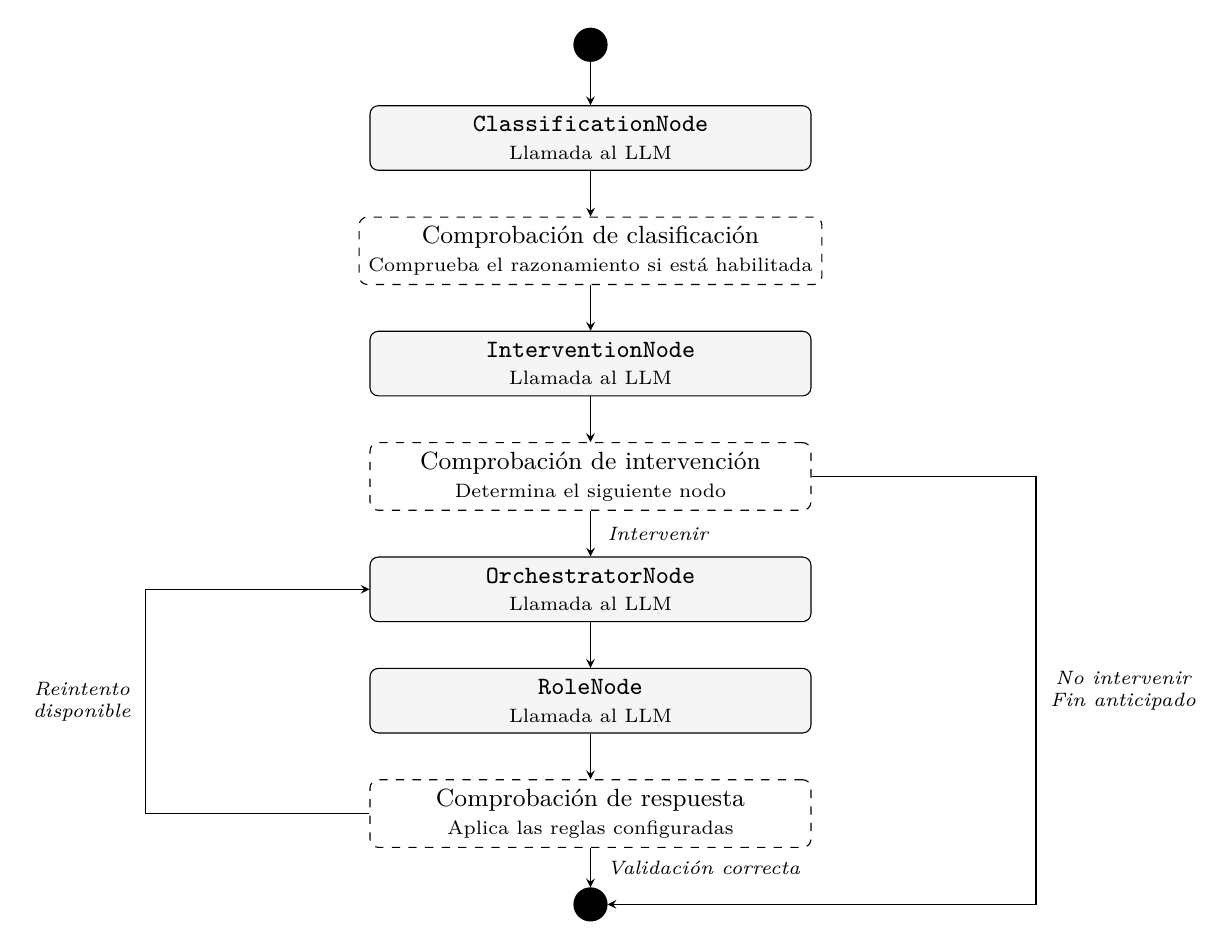
\begin{tikzpicture}[
  node distance=0.58cm,
  box/.style={rectangle, draw, rounded corners=3pt, minimum width=5.6cm,
              minimum height=0.82cm, font=\small, text centered,
              align=center, fill=black!4},
  check/.style={rectangle, draw, dashed, rounded corners=3pt,
                minimum width=5.6cm, minimum height=0.82cm,
                font=\small, text centered, align=center},
  dot/.style={circle, draw, fill=black, minimum size=0.42cm, inner sep=0pt},
  arr/.style={->, >=stealth},
  lbl/.style={font=\scriptsize\itshape, inner sep=2pt, fill=white, align=center}
]

\node[dot]                          (start) {};
\node[box, below=0.55cm of start]   (cls)
  {\texttt{ClassificationNode}\\[-1pt]\scriptsize Llamada al LLM};
\node[check, below=of cls]          (clse)
  {Comprobación de clasificación\\[-1pt]\scriptsize Comprueba el razonamiento si está habilitada};
\node[box, below=of clse]           (int)
  {\texttt{InterventionNode}\\[-1pt]\scriptsize Llamada al LLM};
\node[check, below=of int]          (inte)
  {Comprobación de intervención\\[-1pt]\scriptsize Determina el siguiente nodo};
\node[box, below=of inte]           (orc)
  {\texttt{OrchestratorNode}\\[-1pt]\scriptsize Llamada al LLM};
\node[box, below=of orc]            (rol)
  {\texttt{RoleNode}\\[-1pt]\scriptsize Llamada al LLM};
\node[check, below=of rol]          (respe)
  {Comprobación de respuesta\\[-1pt]\scriptsize Aplica las reglas configuradas};
\node[dot, below=0.5cm of respe]    (end)   {};

\draw[arr] (start) -- (cls);
\draw[arr] (cls)   -- (clse);
\draw[arr] (clse)  -- (int);
\draw[arr] (int)   -- (inte);
\draw[arr] (inte)  -- node[lbl, right=4pt] {Intervenir} (orc);
\draw[arr] (orc)   -- (rol);
\draw[arr] (rol)   -- (respe);
\draw[arr] (respe) -- node[lbl, right=4pt] {Validación correcta} (end);

\coordinate (R1)  at ([xshift=2.85cm] inte.east);
\coordinate (R1b) at (R1 |- end);
\draw[arr] (inte.east) -- (R1)
  -- (R1b)
  node[lbl, midway, right=3pt] {No intervenir\\Fin anticipado}
  -- (end);

\coordinate (L1)  at ([xshift=-2.85cm] respe.west);
\coordinate (L1b) at (L1 |- orc);
\draw[arr] (respe.west) -- (L1)
  -- (L1b)
  node[lbl, midway, left=3pt] {Reintento\\disponible}
  -- (orc.west);

\end{tikzpicture}
\caption{Secuencia de análisis y facilitación. Las cajas con borde continuo representan llamadas al LLM y las cajas con borde discontinuo muestran las comprobaciones internas.}
\label{fig:pipeline}
\end{figure}

Los experimentos no mantienen memoria entre ejecuciones ni guardan un historial de intervenciones. Cada caso se evalúa a partir del contenido registrado en el hilo de discusión. El código contiene una herramienta opcional para consultar el historial en otros modos de ejecución, aunque esa capacidad no forma parte de la evidencia experimental presentada.

El sistema se implementó en Python 3.12 con pydantic-ai\footnote{\url{https://ai.pydantic.dev/}}. Se eligió porque reúne salidas estructuradas, validación con Pydantic, proveedores de LLM distintos y grafos con estado tipado. \texttt{pydantic\_graph} permite representar el grafo de la figura~\ref{fig:pipeline}. Cuando una respuesta no satisface el esquema declarado, la validación detiene esa llamada y permite solicitar una nueva respuesta. La misma secuencia se configuró así con proveedores distintos.

La API REST usa FastAPI y reutiliza los modelos Pydantic para definir los datos que recibe y devuelve. El panel es una aplicación React y la comunicación HTTP con fuentes externas usa httpx.

\subsection{Estado, dependencias y configuración}

La implementación separa las dependencias necesarias para ejecutar el grafo del estado de cada caso. Las dependencias agrupan la configuración, los clientes de los modelos, el acceso a la fuente y el almacenamiento de resultados. El estado conserva el hilo de discusión, la clasificación, la decisión, el rol y la respuesta producidos durante la ejecución. Esta separación permite probar los nodos con servicios controlados y mantener la configuración separada de los resultados.

Las tres interfaces permiten cambiar los servicios conectados sin modificar los nodos y cumplen funciones distintas:

\begin{itemize}
  \item \texttt{LMSBackend} proporciona acceso a las fuentes de hilos de discusión.
  \item \texttt{ModelProvider} obtiene los perfiles de Ollama y OpenRouter.
  \item \texttt{RunResultStore} guarda los resultados en el sistema de archivos o en S3.
\end{itemize}

La secuencia de nodos es fija y conserva los reintentos representados en la figura~\ref{fig:pipeline}.

Además, se puede configurar un modelo distinto para la clasificación, la decisión de intervención, la selección del rol y la generación de la respuesta. Si una etapa no tiene un modelo específico, utiliza el modelo configurado por defecto. Esta opción permite asignar modelos diferentes según la función de cada etapa.

\subsection{Salidas estructuradas, validación y reintentos}

Los agentes devuelven respuestas divididas en campos definidos que el sistema puede validar y conservar. Estas respuestas se denominan salidas estructuradas. Como los modelos locales y externos no ofrecen el mismo soporte para generarlas, cada configuración indica si el esquema se proporciona como una herramienta o como una instrucción textual. Los perfiles evaluados de Qwen 3.5 y Ministral 3 usan la instrucción textual, mientras que los perfiles externos usan el esquema como herramienta. Los experimentos no aislaron el efecto de esta diferencia sobre la finalización ni sobre la calidad de las intervenciones.

Antes de entregar la respuesta, el agente de rol verifica que el texto no esté vacío, que indique la técnica aplicada y que no contenga ciertas expresiones de evaluación o calificación. Si alguna comprobación falla y quedan intentos, devuelve el control al orquestador con una descripción del problema. El orquestador recibe esa información y se le pide elegir un rol distinto, por lo que un reintento puede cambiar tanto el rol como la respuesta.

Si una salida no cumple el esquema, el modelo recibe el error de validación y puede reintentar. Si una etapa posterior falla, el resultado conserva las decisiones ya producidas. Cuando el agente de rol agota sus reintentos, conserva además el historial parcial de mensajes. El panel puede mostrar así dónde se detuvo el caso y qué había producido el modelo.

\section{Estrategia de contexto y prompts}
\label{sec:prompts}

La información que recibe cada etapa forma parte del control de la ejecución. En este trabajo, la estrategia de contexto determina la información que recibe cada agente, las decisiones anteriores que se transmiten entre etapas y las herramientas disponibles durante la ejecución. Esta estrategia corresponde al concepto de ingeniería del contexto presentado en el estado del arte. Su implementación incluye el estado compartido, el contexto específico del rol, el acceso al repertorio de técnicas y la reducción del volumen de información antes de generar la respuesta.

El \textit{prompt} es el conjunto de instrucciones que se envía al modelo. Para mantener un criterio común entre los agentes, los prompts del sistema siguen una estructura de cuatro secciones. \texttt{Persona} define la identidad del agente, que es breve para los nodos internos y más detallada para los agentes que producen texto dirigido al estudiante. \texttt{Constraints} declara los límites de responsabilidad y las restricciones de comportamiento. \texttt{Context} contiene la información variable de cada ejecución, como los umbrales configurables, el contenido del hilo de discusión y las marcas de tiempo. Finalmente, \texttt{Task} describe la salida que debe producir el agente y el procedimiento que debe seguir \parencite{SikstromEtAl2022}.

El prompt del agente clasificador ilustra cómo se aplica esta estructura.

\begin{small}
\begin{verbatim}
# Persona
You are a learning scientist reading an asynchronous academic
discussion thread.

# Constraints
You do not decide whether to intervene - that belongs to the next
pipeline node. Accuracy here determines everything downstream.

# Context
Discussion context: {discussion_context}
Current timestamp: {current_timestamp}
Stalled threshold: {stalled_threshold_hours} hours without new posts

# Task
Read the thread and produce a structured classification across five
fields: state, trajectory, participation balance, discourse quality,
and inquiry phase.
\end{verbatim}
\end{small}

Durante una ejecución, las variables anteriores se completan y el contenido del hilo de discusión se envía como mensaje de entrada. El siguiente extracto abreviado procede del escenario \texttt{new}, ejecutado con \texttt{ollama:ministral-3:14b} en la serie de ejecuciones realizada en Idril e identificada como \texttt{2026-07-23T11-51-18-threads-4-models}:

\begin{small}
\begin{verbatim}
Current timestamp: 2026-07-23T11:51:47+00:00
Topic: Privacy implications of large language models
Learning objectives:
- Identify privacy risks in LLM training data
- Evaluate current mitigation strategies
- Propose privacy-preserving alternatives

Posts:
- [2026-03-12T13:00:00+00:00] Prof. Garcia:
  This week we're discussing privacy in LLMs. What are the main
  risks when personal data appears in training sets?
\end{verbatim}
\end{small}

El modelo devolvió una instancia del esquema de clasificación con los siguientes valores:

\begin{itemize}
  \item Estado: \texttt{new}.
  \item Trayectoria: \texttt{never\_started}.
  \item Participación: \texttt{instructor\_centered}.
  \item Calidad del discurso: \texttt{formulaic}.
  \item Fase de indagación: \texttt{triggering}.
\end{itemize}

El registro de la ejecución conserva el prompt del sistema, este mensaje, la salida estructurada y el razonamiento. El ejemplo muestra cómo la plantilla se combina con el contexto de un hilo de discusión concreto.

El texto del hilo de discusión forma parte del mensaje que recibe el modelo. La implementación no identifica si una publicación contiene instrucciones dirigidas al modelo, y los experimentos no incluyeron casos de ese tipo.

Los agentes de rol tienen una sección Persona más elaborada, con un perfil que define el tono y el registro de la respuesta; los nodos internos mantienen esa caracterización al mínimo.

Los agentes de rol consultan el repertorio de técnicas mediante una función disponible durante la ejecución. De este modo, el repertorio no se incluye completo en las instrucciones iniciales. Se construyó a partir de las fuentes revisadas y conserva la categoría de origen de cada técnica. La función devuelve todas las técnicas sin filtrar por rol ni por estado, y cada entrada contiene el nombre, la descripción y un ejemplo. En la configuración actual, la generación de la respuesta exige realizar esta consulta. Por ello, un modelo que no pueda utilizar funciones externas puede completar las primeras decisiones, aunque no puede generar la respuesta.

El agente de rol dispone también de dos consultas opcionales. \path{get_course_context} solicita a la fuente configurada el nombre del curso y su estructura de secciones y secuencias. Si la fuente o el dato no están disponibles, la función informa de su ausencia. La búsqueda web utiliza el tema de la discusión para localizar ejemplos, definiciones o material de referencia. El agente decide si necesita estas consultas para seleccionar la técnica o el tono de la respuesta.

El agente de rol reduce el volumen de información acortando el razonamiento recibido de las etapas anteriores y utilizando un ejemplo por técnica. Ante errores menores de formato, intenta corregir la salida estructurada antes de descartarla. Las consultas externas devuelven un error descriptivo si su servicio no está disponible.

El código limita a una consulta por respuesta el acceso a las técnicas y al historial. Así se evita incorporar varias veces la misma información al contexto.

\section{Ejecución e inspección del panel}
\label{sec:prototipo-inspeccion}

La interfaz permite iniciar los análisis y consultar los resultados de la ejecución interna descrita en las secciones anteriores. El panel permite seleccionar la fuente de los hilos de discusión y los modelos, iniciar una ejecución y revisar las decisiones conservadas en cada etapa. Los resultados se guardan para su consulta. El panel no publica intervenciones.

Al abrir el detalle de un hilo de discusión, el panel muestra la discusión completa, la clasificación del modelo con su confianza y razonamiento, la acción sugerida con el rol y la técnica y, cuando se decide intervenir, el borrador de respuesta (figura~\ref{fig:thread-analysis}). Esta organización permite revisar la decisión de intervenir antes de examinar el texto generado. La barra lateral incluye un enlace a Logfire para consultar el registro técnico de la ejecución.

\begin{figure}[htbp]
\centering
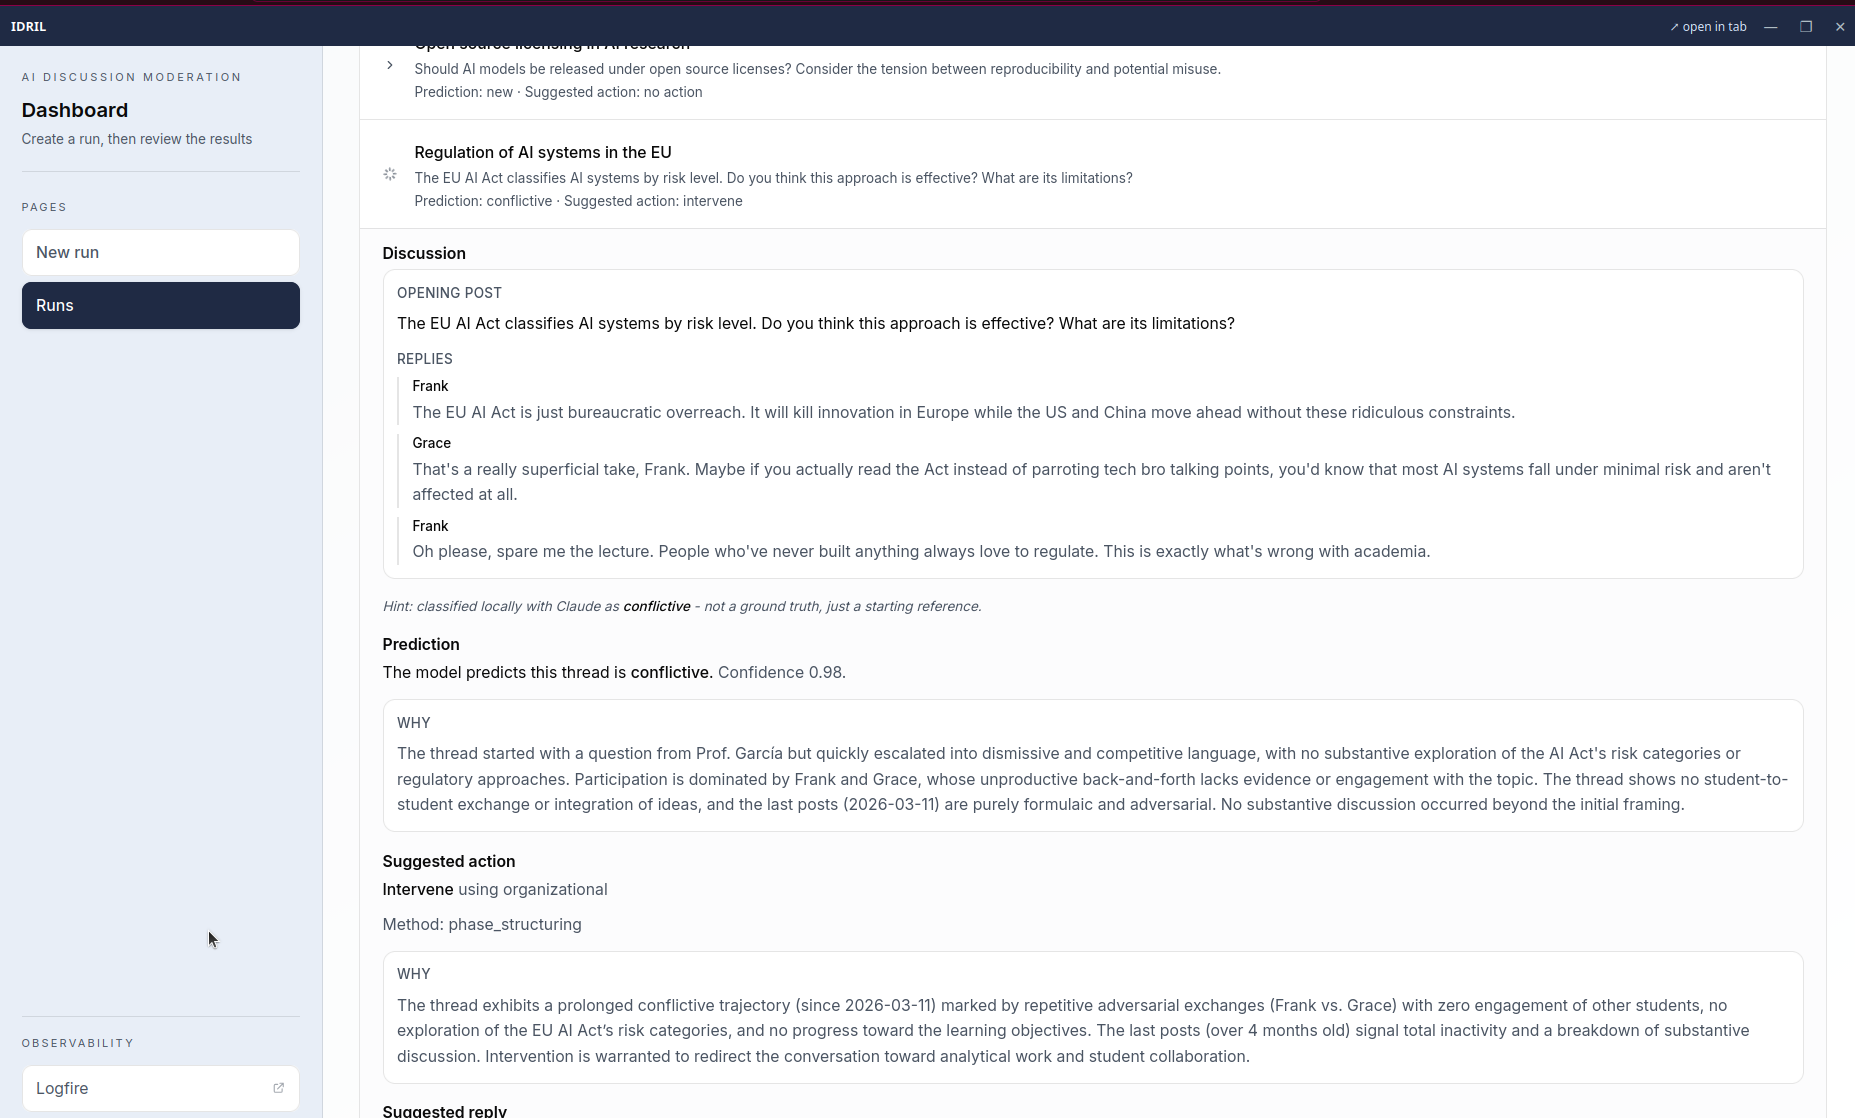
\includegraphics[width=0.95\textwidth]{figures/dashboard-thread-analysis-latest}
\caption{Detalle del análisis de un hilo de discusión, con la clasificación y la acción sugerida.}
\label{fig:thread-analysis}
\end{figure}

La información disponible para inspeccionar una ejecución se conserva en dos lugares. El resultado contiene los mensajes de cada nodo y permite mostrarlos en el panel. Por su parte, los registros de Logfire permiten consultar la duración, las consultas realizadas y los errores de validación. La figura~\ref{fig:logfire-development} muestra el registro de una ejecución completa y la figura~\ref{fig:logfire-model-call} presenta el detalle de una llamada al modelo, incluida su entrada y su salida estructurada. El registro en Logfire es opcional y la secuencia puede ejecutarse sin sus credenciales.

\begin{landscape}
\begin{figure}[p]
\centering
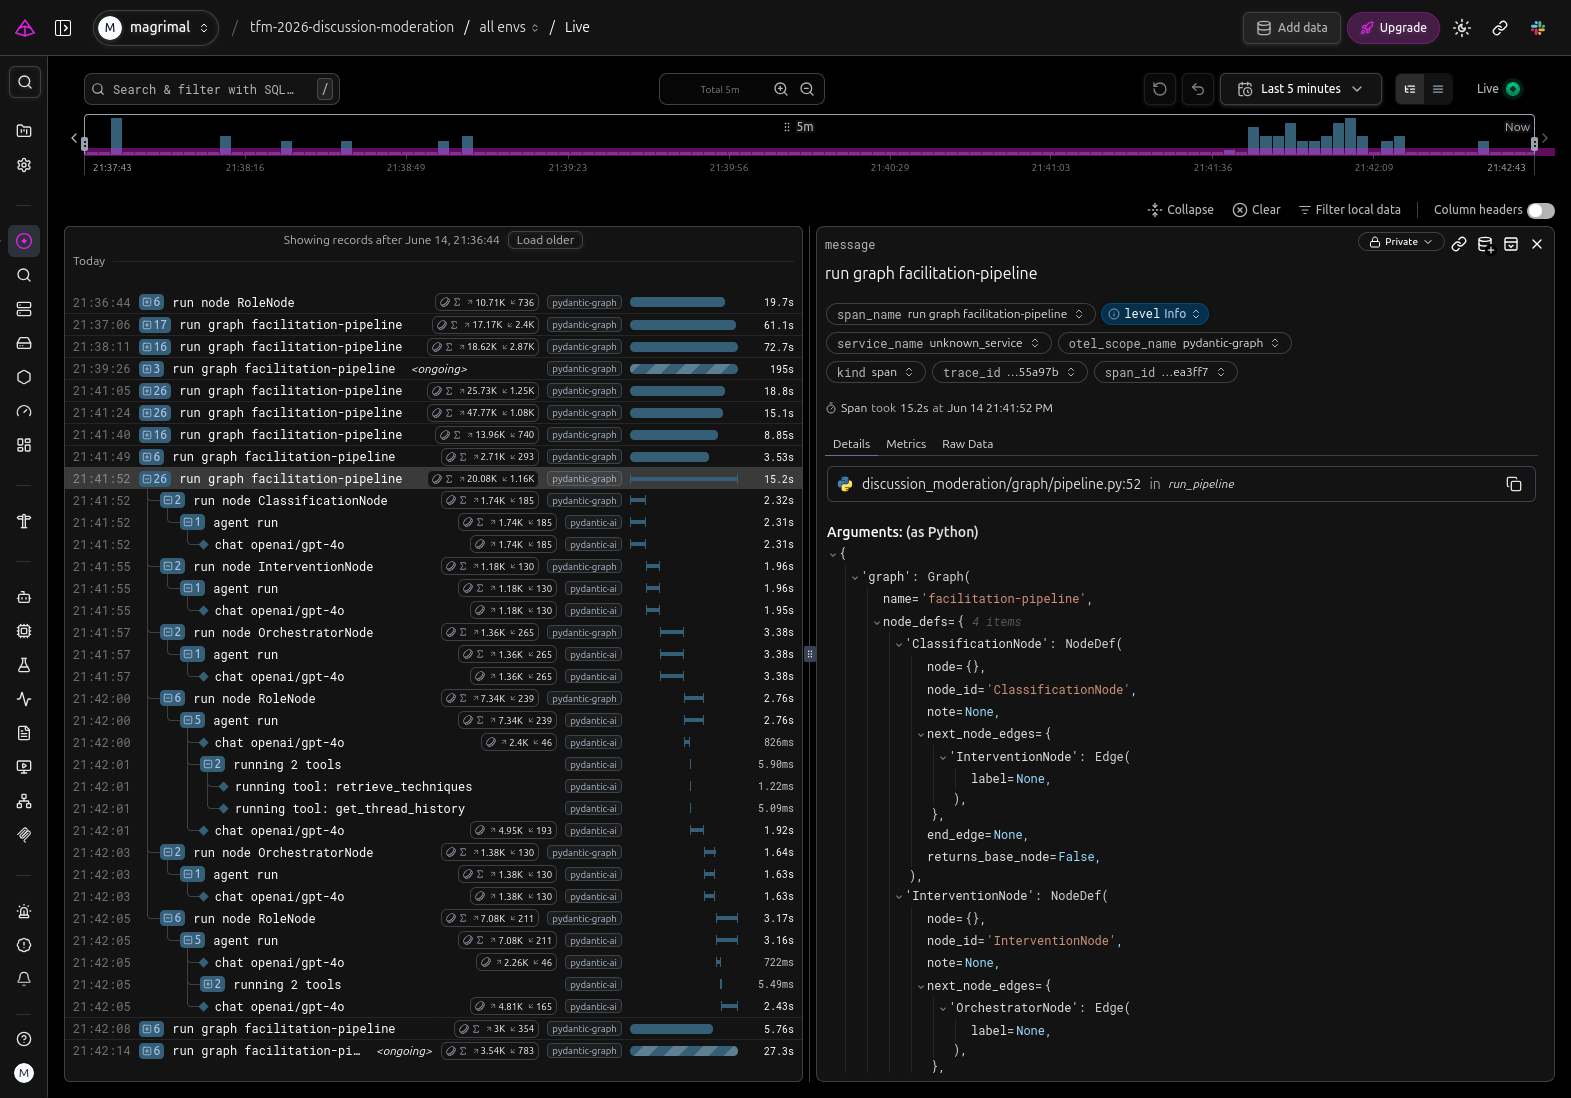
\includegraphics[width=0.95\linewidth]{figures/logfire-trace}
\caption{Registro de una ejecución en Logfire, con las llamadas correspondientes a cada etapa.}
\label{fig:logfire-development}
\end{figure}
\end{landscape}

\begin{landscape}
\begin{figure}[p]
\centering
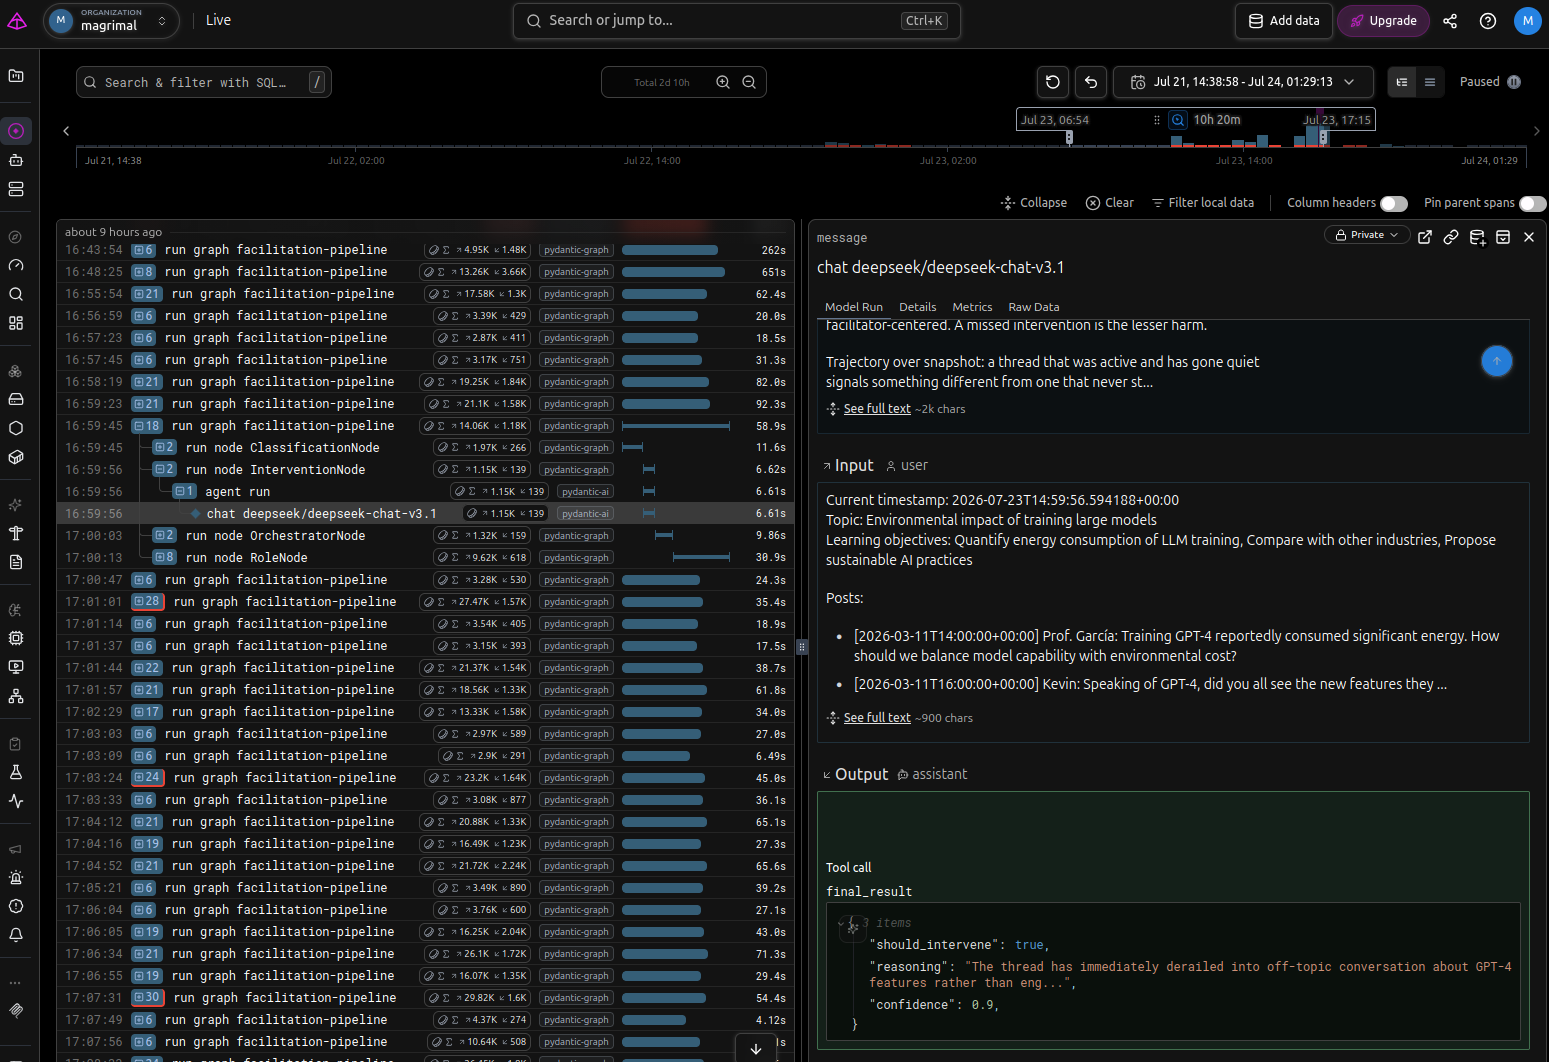
\includegraphics[width=0.95\linewidth]{figures/logfire-model-call-detail.png}
\caption{Detalle de una llamada al modelo registrada en Logfire. La vista muestra el modelo utilizado, el hilo de discusión enviado como entrada y la decisión estructurada producida por el agente.}
\label{fig:logfire-model-call}
\end{figure}
\end{landscape}

El anexo~\ref{app:flujo-prototipo} documenta los pasos de uso de la interfaz, desde la página de acceso hasta la selección de hilos de discusión y la consulta de resultados.

\FloatBarrier
\section{Despliegue y entornos de ejecución}
\label{sec:entornos-ejecucion}

Para ejecutar los experimentos, el sistema se desplegó en dos entornos (tabla~\ref{tab:environment-config}). Idril es un servidor de la UCM utilizado con modelos locales. El segundo entorno es una instancia de Amazon Elastic Compute Cloud (AWS EC2) que accede a modelos externos. Cada instalación incluye el panel React, la API FastAPI y la secuencia de facilitación descrita en este capítulo. Las configuraciones difieren en el proveedor de modelos y en el tiempo máximo de ejecución.

El repositorio contiene el \texttt{Containerfile}, \texttt{docker-compose.yml}, los objetivos de \texttt{Make} y los programas de arranque y reinicio. Los archivos de configuración de Idril y EC2 contienen credenciales, direcciones y valores específicos de cada instalación, por lo que no se versionan. El repositorio proporciona una plantilla para desarrollo local. Para reproducir los despliegues descritos se necesita completar esa plantilla con una configuración equivalente.

Ambos entornos ejecutan la misma secuencia y utilizan su propio proveedor, catálogo de modelos y tiempo máximo. Los manifiestos experimentales se recuperan del mismo espacio de almacenamiento y prefijo en Amazon S3. Además, Logfire conserva los registros técnicos de las dos instalaciones.

\begin{table}[htbp]
\centering
\small
\renewcommand{\arraystretch}{1.16}
\begin{tabularx}{\textwidth}{@{}Z{3.2cm}YY@{}}
\toprule
\textbf{Configuración} & \textbf{Idril} & \textbf{AWS EC2} \\
\midrule
Proveedor & Ollama en la red universitaria & OpenRouter \\
Modelo base & Ministral 3 14B & GPT-4o \\
Catálogo evaluado & Ministral 3 14B y 8B; Qwen 3.5 27B y 9B & GPT-4o, Claude Haiku 4.5, GPT-4o-mini y DeepSeek V3.1 \\
Ruta de la API & Raíz del despliegue & Prefijo \texttt{/api} \\
Resultados & Mismo almacenamiento y prefijo en Amazon S3 & Mismo almacenamiento y prefijo en Amazon S3 \\
Registro técnico & Logfire & Logfire \\
\bottomrule
\end{tabularx}
\caption{Diferencias y elementos compartidos entre las configuraciones desplegadas.}
\label{tab:environment-config}
\end{table}

\subsection{Idril: modelos locales}

Idril es un servidor con Debian Linux, 28 CPU, 128 GB de memoria RAM y una GPU NVIDIA RTX 4000 con 20 GB de VRAM. La GPU permite servir mediante Ollama los modelos que se ejecutan en infraestructura de la universidad. El panel y la API se despliegan en el mismo servidor y son accesibles dentro de la red de la UCM.

\begin{figure}[htbp]
\centering
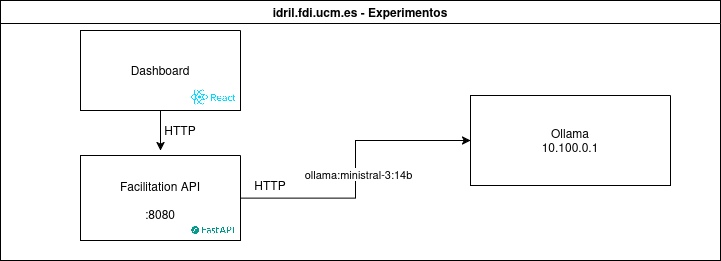
\includegraphics[width=0.92\textwidth]{figures/deployment-idril-experiments.png}
\caption{Despliegue utilizado en Idril para los experimentos con modelos locales. El panel se comunica con la API de facilitación, que envía las solicitudes a Ollama dentro de la red de la UCM.}
\label{fig:deployment-idril-experiments}
\end{figure}

Este entorno se reserva a perfiles de modelos locales. Su catálogo experimental incluye dos tamaños de Ministral 3 y dos de Qwen 3.5. La lista disponible y el modo de extracción estructurada se pueden ajustar de forma independiente a las pruebas con APIs externas. Los tiempos de ejecución de ambos entornos no son directamente comparables. En Idril incluyen la inferencia realizada en el servidor local, mientras que en EC2 dependen de los servicios externos utilizados mediante OpenRouter.

\subsection{AWS EC2: modelos externos}

La instalación de AWS EC2 ejecuta el mismo panel y la misma API. En este entorno, el servicio envía las solicitudes a OpenRouter, que proporciona acceso a GPT-4o, Claude Haiku 4.5, GPT-4o-mini y DeepSeek V3.1 mediante una API común. Sus registros permiten comprobar qué proveedor atendió una llamada, los tokens consumidos, la velocidad y el coste.

EC2 permitió ejecutar las pruebas con modelos externos de forma independiente a Idril. También proporcionó un entorno accesible fuera de la red universitaria para mostrar el panel. El acceso a la aplicación estuvo protegido mediante autenticación HTTP básica. La procedencia de los hilos de discusión se mantuvo fuera de la comparación entre proveedores.

\begin{landscape}
\begin{figure}[p]
\centering
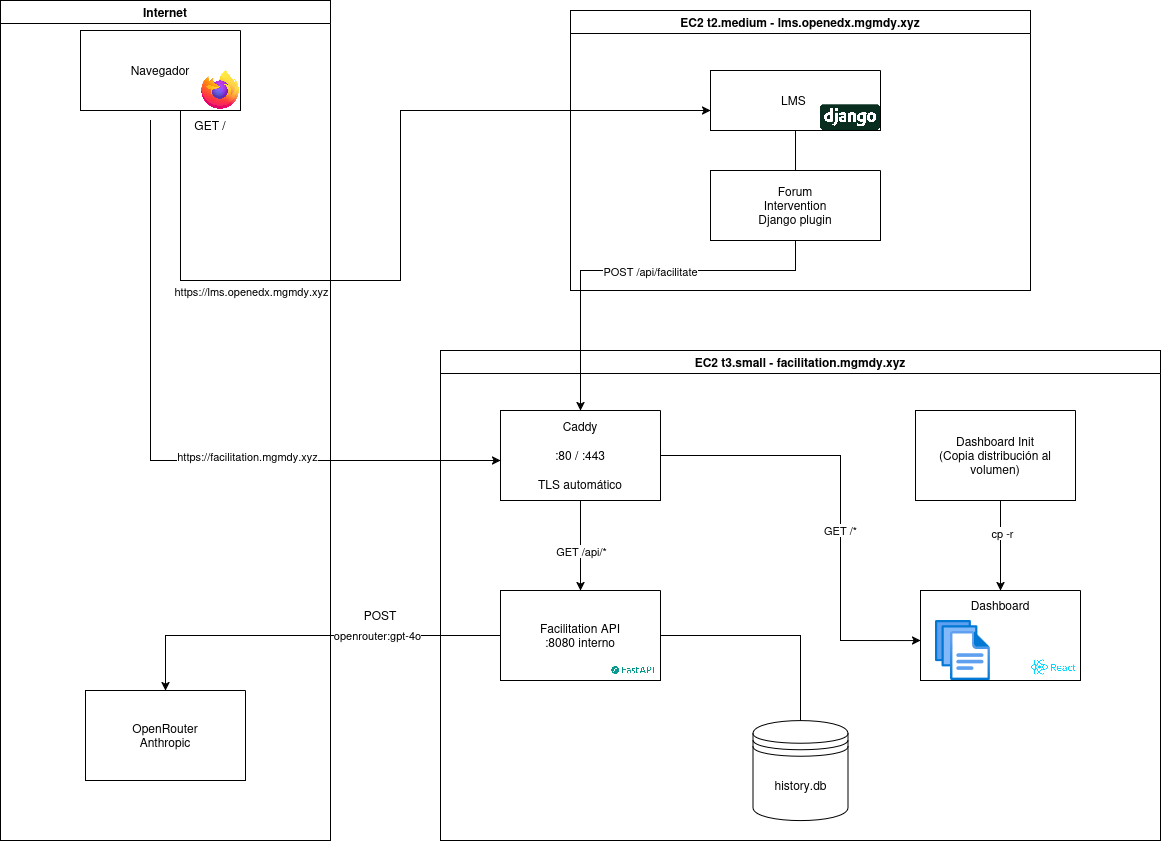
\includegraphics[width=0.87\linewidth]{figures/deployment-aws-openedx-facilitation.png}
\caption{Despliegue en AWS utilizado para la prueba de concepto con Open edX y las ejecuciones con modelos externos. El complemento de Open edX se comunica con la API de facilitación, y el servicio accede a los proveedores de modelos externos.}
\label{fig:deployment-aws-openedx-facilitation}
\end{figure}
\end{landscape}

El capítulo siguiente analiza conjuntamente las ejecuciones y conserva la procedencia de cada una.

\chapter{Resultados}

Este capítulo presenta los resultados obtenidos con el sistema descrito en el capítulo anterior, y los contrasta con los objetivos y la motivación planteados en la introducción. La evaluación se organiza en cuatro capas complementarias, ordenadas por coste y profundidad, seguidas de una discusión que conecta lo observado con las preguntas de investigación. Las capas 1 y 2 están implementadas de forma completa. La capa 3 está implementada de forma preliminar para un subconjunto de escenarios y modelos. La capa 4 se aplicó como revisión manual exploratoria, y su versión formal con doble anotación independiente queda como trabajo futuro.

\section{Capa 1: Aserciones estructurales}

La primera capa verifica que la salida del pipeline cumple condiciones básicas con independencia del contenido del hilo. Antes de que el resultado salga del pipeline se comprueba que la respuesta no está vacía, que la técnica pertenece al repertorio conocido, que el valor de confianza está en el rango válido y que las flags de escalado al instructor y de publicación en el hilo son coherentes entre sí; durante la generación del texto, el agente de rol detecta presencia de lenguaje evaluativo y técnica no especificada. Cuando cualquiera de estas comprobaciones falla, el sistema activa el circuito de retroalimentación y reintenta la generación con el feedback incluido en el contexto, hasta un máximo de tres intentos.

Estas comprobaciones no son suficientes para determinar si una respuesta es pedagógicamente adecuada. Una respuesta puede pasar todas las verificaciones y seguir siendo inapropiada si la técnica está mal aplicada al contexto o el texto no está fundamentado en las contribuciones del hilo. Para eso están las capas siguientes.

\section{Capa 2: Evaluación con escenarios de prueba}

La segunda capa evalúa el comportamiento del sistema contra ocho escenarios de discusión definidos en código, en \texttt{discussion\_moderation/evals/fixtures/}, y ejecuta el pipeline de forma reproducible contra cada uno.

Seis escenarios cubren uno a uno los estados de la taxonomía (nueva, activa, estancada, conflictiva, convergente y fuera de tema), diseñados para que el clasificador los asigne sin ambigüedad. De esos seis, solo dos producen intervención; dos escenarios adicionales cubren ese espacio. El primero representa un hilo con participación distribuida pero discurso formulaico, donde ningún estudiante desarrolla argumentos ni conecta ideas con las lecturas del curso, y activa el rol intelectual. El segundo representa un hilo donde un participante domina la discusión con varias contribuciones sustantivas y el resto solo asiente brevemente, y activa el rol social. Todos los escenarios comparten el mismo contexto de curso y una marca de tiempo fija para que los resultados sean comparables entre modelos y entre fechas.

La herramienta registra la clasificación obtenida, la decisión de intervención, el rol seleccionado si hubo intervención y si la respuesta superó la validación. Esta capa verifica que el modelo completa el pipeline sin errores y que sus clasificaciones son coherentes con el estado diseñado para cada escenario, pero no evalúa la calidad pedagógica de las respuestas.

Los experimentos descritos en este apartado se ejecutaron el 14 de junio de 2026 contra los ocho escenarios con dos modelos externos (\texttt{openrouter:openai/gpt-4o} y \texttt{openrouter:anthropic/claude-sonnet-4.5}) y un modelo local en Idril (\texttt{ollama:ministral-3:14b}). La tabla~\ref{tab:resultados-fixtures} recoge los resultados obtenidos para cada escenario.

\begin{table}[h]
\centering
\small
\begin{tabular}{llllllll}
\toprule
\textbf{Escenario} & \textbf{Estado esperado} & \multicolumn{2}{c}{\textbf{gpt-4o}} & \multicolumn{2}{c}{\textbf{claude-sonnet-4.5}} & \multicolumn{2}{c}{\textbf{ministral-3-14b}} \\
 & & Estado & Interviene & Estado & Interviene & Estado & Interviene \\
\midrule
new              & nueva         & nueva       & sí   & estancada   & sí & nueva      & no \\
active           & activa        & activa      & no   & estancada   & sí & activa     & no \\
stalled          & estancada     & nueva       & no   & estancada   & sí & estancada  & sí \\
conflictive      & conflictiva   & conflictiva & sí   & conflictiva & sí & conflictiva & sí \\
convergent       & convergente   & activa      & no   & estancada   & sí & convergente & no \\
off\_topic       & fuera de tema & fuera de tema & sí & fuera de tema & sí & —         & — \\
shallow\_discourse & superficial  & convergente & no   & estancada   & sí & estancada & sí \\
dominated        & dominada      & estancada   & no   & —           & — & estancada & no \\
\midrule
\textbf{Correctos} & & \textbf{4/8} & \textbf{4/8} & \textbf{3/7} & \textbf{4/7} & \textbf{5/8} & \textbf{7/8} \\
\bottomrule
\end{tabular}
\caption{Clasificación e intervención sobre los ocho escenarios de prueba. — indica ejecución incompleta. Correcto: valor obtenido coincide con el esperado.}
\label{tab:resultados-fixtures}
\end{table}

Adicionalmente se ejecutó un experimento contra seis hilos reales del curso \texttt{course-v1:openedx+PROG+2026}, recogidos directamente de la instancia de Open edX. La tabla~\ref{tab:resultados-lms} muestra la clasificación y la decisión de intervención producidas por cada modelo para cada hilo. En este caso no existe estado esperado definido, ya que los hilos provienen de actividad real de estudiantes.

\begin{table}[h]
\centering
\small
\begin{tabular}{p{4.8cm}llll}
\toprule
\textbf{Hilo} & \multicolumn{2}{c}{\textbf{gpt-4o}} & \multicolumn{2}{c}{\textbf{claude-sonnet-4.5}} \\
 & Estado & Rol & Estado & Rol \\
\midrule
Extensión de plazo (anuncio) & estancada & afectivo & fuera de tema & — \\
Peer assessment (conflicto) & conflictiva & moderador & conflictiva & moderador \\
Test demasiado difícil       & estancada & organizacional & conflictiva & organizacional \\
¿Cómo obtuvimos 59?          & convergente & — & estancada & intelectual \\
Error en el examen semana 1  & nueva & organizacional & fuera de tema & — \\
Knowing vs Doing             & conflictiva & — & estancada & intelectual \\
\bottomrule
\end{tabular}
\caption{Clasificación y rol sobre seis hilos reales del curso PROG 2026. — indica no intervención.}
\label{tab:resultados-lms}
\end{table}

\begin{figure}[!ht]
\centering
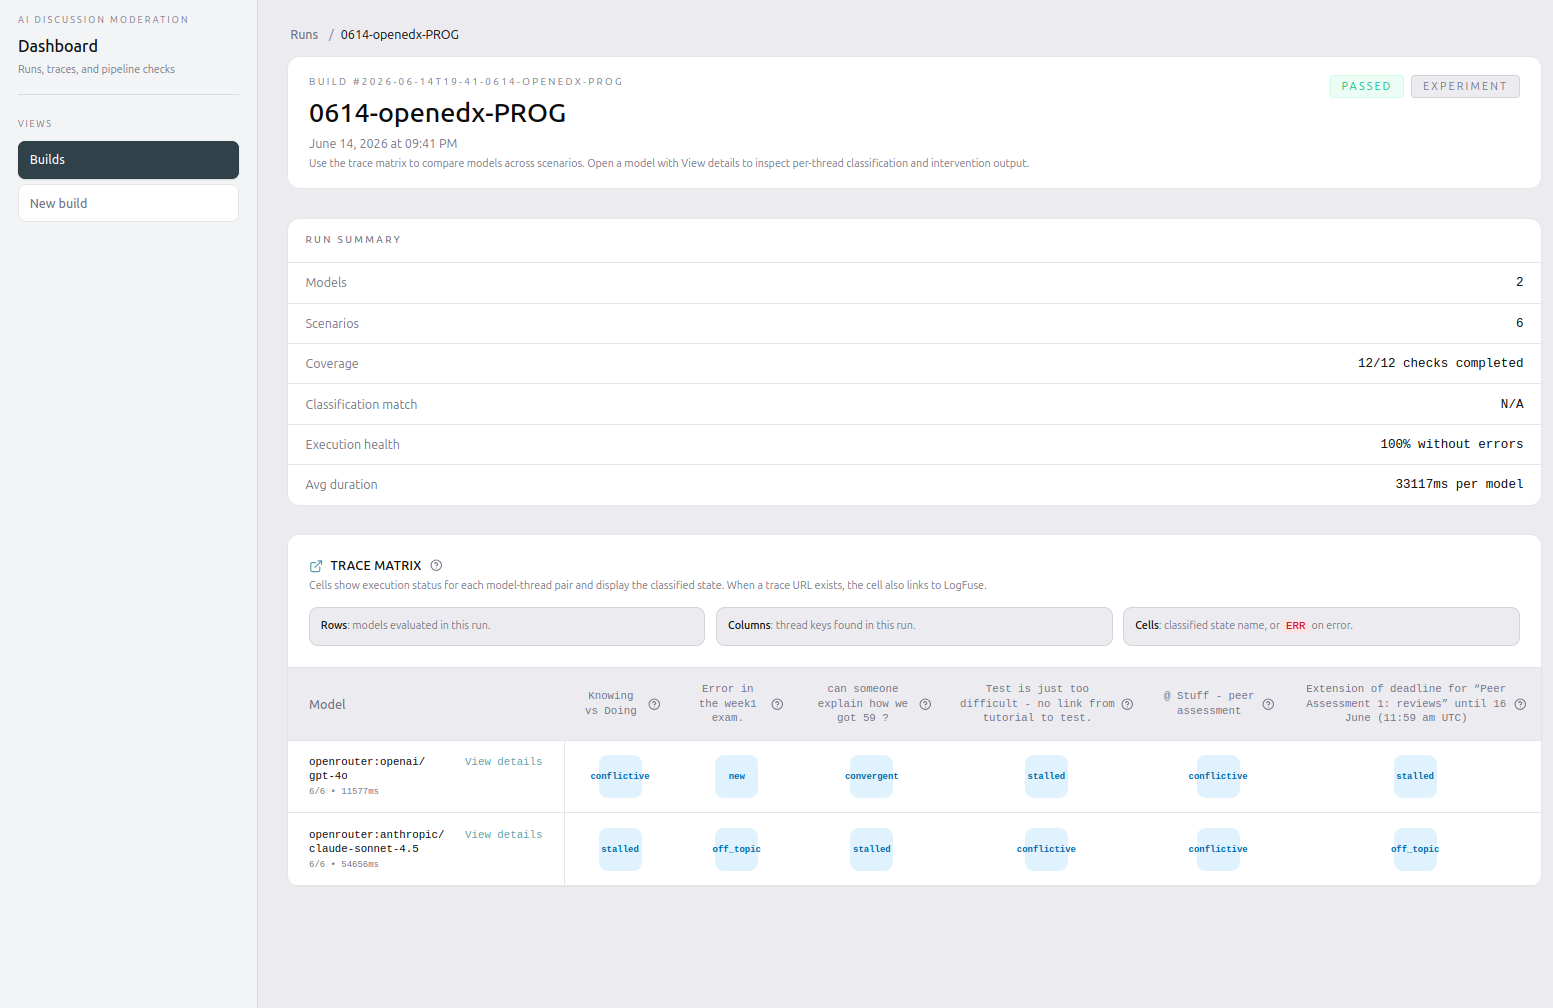
\includegraphics[width=0.9\textwidth]{figures/dashboard-trace-lms}
\caption{Matriz de trazas del run PROG: dos modelos × seis hilos reales del curso.}
\label{fig:dashboard-trace-lms}
\end{figure}

La tabla~\ref{tab:costes-experimentos} recoge el desglose de coste y uso de tokens por modelo para el conjunto de experimentos del 14 de junio.

\begin{table}[h]
\centering
\small
\begin{tabular}{lrrrrr}
\toprule
\textbf{Modelo} & \textbf{Llamadas} & \textbf{Tokens entrada} & \textbf{Tokens salida} & \textbf{Latencia media} & \textbf{Coste total} \\
\midrule
gpt-4o              & 61 & 162.229 & 8.733  & 1,7 s  & \$0,49 \\
claude-sonnet-4.5   & 60 & 237.761 & 31.349 & 12,2 s & \$1,18 \\
ministral-3-14b (Idril) & 8 & 58.012 & 11.306 & 82,8 s & N/A (local) \\
\midrule
\textbf{Total OpenRouter}      & 121 & 399.990 & 40.082 & — & \$1,68 \\
\bottomrule
\end{tabular}
\caption{Coste y uso de tokens por modelo, experimentos del 14 de junio de 2026.}
\label{tab:costes-experimentos}
\end{table}

El panel de evaluación descrito en el capítulo anterior permite lanzar experimentos, filtrar resultados por modelo o escenario e inspeccionar trazas desde el navegador sin necesitar acceso SSH a ninguno de los dos entornos.

\section{Capa 3: Clasificación automática con LLM}

La tercera capa aplica una clasificación automática con LLM sobre las salidas del pipeline para verificar coherencia entre estado del hilo, decisión de intervención y rol seleccionado. En esta capa se registra si la salida es consistente con la taxonomía de estados definida y si la decisión tomada corresponde al patrón de participación observado en el hilo. En este trabajo, esta capa se aplicó de forma preliminar sobre un subconjunto de pares modelo-hilo para detectar fallos sistemáticos de clasificación y de selección de rol.

\section{Capa 4: Revisión manual y anotación por expertos}

En la ejecución actual se realizó una revisión manual exploratoria de salidas para contrastar la clasificación automática y verificar coherencia entre estado clasificado, técnica seleccionada y tono de la intervención. Para eso se usaron dos herramientas. El panel de evaluación permite inspeccionar el contenido del hilo y la intervención generada en una sola vista. Logfire expone la traza completa de cada ejecución, incluyendo los mensajes enviados a cada agente y sus respuestas. Esta revisión permitió identificar errores de aplicación de técnica y casos límite no detectados por aserciones estructurales.

\begin{figure}[!ht]
\centering
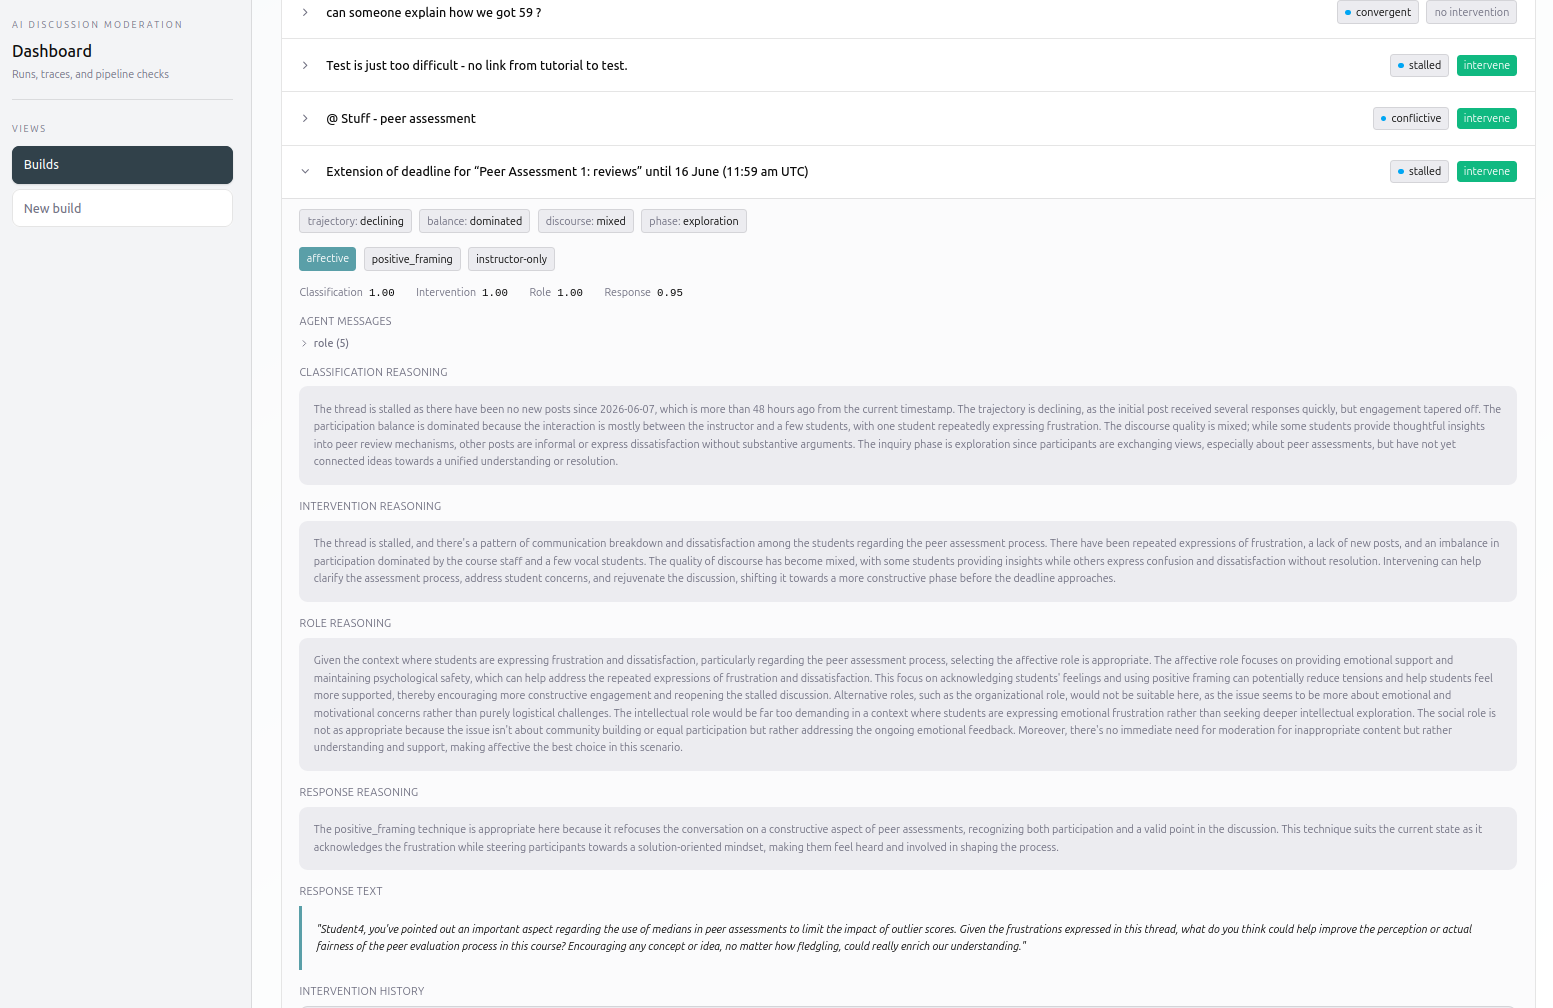
\includegraphics[width=0.85\textwidth]{figures/dashboard-thread-detail}
\caption{Detalle de un hilo en el panel: contenido, clasificación e intervención generada.}
\label{fig:dashboard-thread-detail}
\end{figure}

\begin{figure}[!ht]
\centering
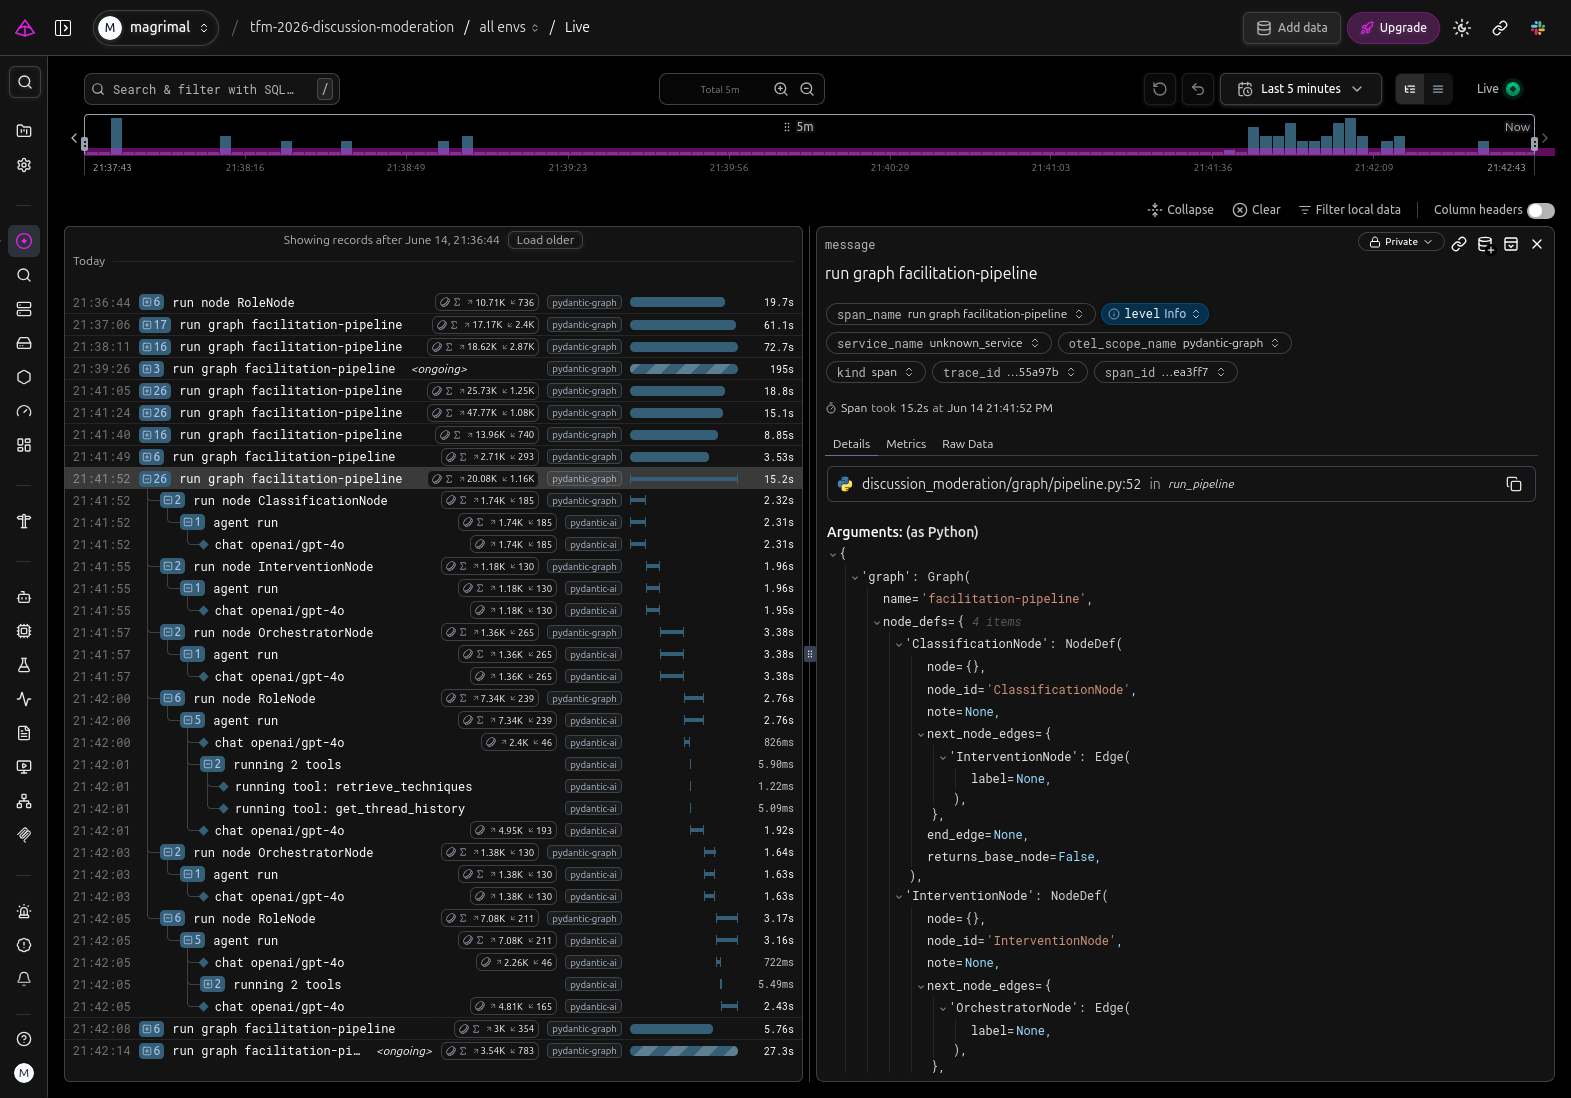
\includegraphics[width=0.85\textwidth]{figures/logfire-trace}
\caption{Trazas del pipeline de facilitación en Logfire.}
\label{fig:logfire-trace}
\end{figure}

La versión formal de esta capa, con anotación de veinte a treinta pares (hilo, respuesta) por dos anotadores independientes, cálculo de acuerdo inter-anotador mediante kappa de Cohen y resolución por consenso de desacuerdos, se define como trabajo futuro.

\section{Ejemplos de intervención}

\textit{Pendiente: esta sección debe incluir dos o tres ejemplos completos de intervención (hilo de entrada, clasificación producida y texto generado) que ilustren cada rol de facilitación, extraídos de una ejecución real del panel de evaluación. Queda pendiente de la ejecución de nuevos experimentos.}

\section{Discusión}

Los resultados de las capas 1 y 2 muestran que el pipeline completa su ciclo de clasificación, decisión e intervención de forma consistente, pero también que la precisión de clasificación varía sustancialmente entre modelos, de 3/7 a 7/8 escenarios correctos según el modelo evaluado. Esta variación responde directamente al primer objetivo específico del trabajo, producir intervenciones coherentes con el tema y la continuidad de la discusión dentro de tiempos y consumo de recursos razonables, y muestra que ese objetivo depende tanto del diseño del pipeline como de la elección de modelo, no solo del primero.

La tabla de hilos reales del curso PROG 2026 confirma que el sistema opera sobre discusiones no controladas, aunque sin estado esperado no es posible calcular una tasa de acierto sobre esos casos; la discrepancia entre modelos en la misma tabla (por ejemplo, \textit{Test demasiado difícil} clasificado como estancada por un modelo y como conflictiva por otro) es evidencia de que la clasificación de estado sigue siendo la etapa más sensible del pipeline, consistente con lo observado en los escenarios de prueba.

La tabla de costes muestra que la latencia del modelo local en Idril (82,8 s de media) es incompatible con un ciclo de facilitación interactivo, mientras que los modelos externos completan el ciclo en segundos a un coste bajo por intervención (entre \$0,008 y \$0,02 por llamada). Esta diferencia justifica la separación de entornos descrita en el capítulo anterior, experimentación con modelos locales en un entorno, facilitación en producción con modelos externos en otro.

En conjunto, la evidencia reunida en este capítulo respalda una afirmación acotada, el artefacto produce clasificaciones e intervenciones coherentes y auditables en escenarios controlados y sobre hilos reales, con una fiabilidad de clasificación que depende del modelo. No respalda una afirmación de efectividad pedagógica ni de impacto en aprendizaje, que exige la validación con estudiantes reales descrita como trabajo futuro en las conclusiones.

\chapter{Conclusiones}
\label{chap:conclusiones}

Este trabajo partió de la pregunta de si la facilitación humana de una discusión puede describirse con suficiente claridad para implementarla como un sistema. La revisión de la literatura permitió dividir el proceso en decisiones observables. A partir de ellas, se implementó un sistema que recibe un hilo de discusión, analiza su estado, decide si corresponde intervenir y genera una respuesta candidata cuando la intervención está justificada.

\section{Cumplimiento de los objetivos}

El objetivo principal era diseñar e implementar un sistema basado en LLMs y técnicas de ingeniería del contexto para analizar y facilitar discusiones académicas asíncronas procedentes de distintas fuentes. Este objetivo se cumplió en lo relativo al diseño y la implementación. El sistema utiliza el contenido del hilo de discusión, los objetivos de aprendizaje cuando se proporcionan y criterios derivados de la literatura para decidir si intervenir y producir una respuesta candidata. El contrato de entrada permite incorporar otra fuente mediante un adaptador, aunque esta posibilidad no se verificó con un segundo LMS o foro.

Los experimentos aportan evidencia de viabilidad técnica sobre ese objetivo porque la secuencia de facilitación se ejecutó con modelos locales y externos. Además, como las contribuciones se producen en momentos distintos, el sistema puede realizar el análisis en segundo plano y la ejecución no requiere una respuesta conversacional en tiempo real.

Los experimentos documentan la ejecución técnica del sistema. Sin embargo, la evaluación no incluyó estudiantes, instructores ni cursos en funcionamiento, por lo que no permite establecer efectos sobre el aprendizaje, la carga docente o la capacidad de atender más discusiones.

El primer objetivo específico proponía un sistema de agentes organizado en etapas. Cada etapa concentra una responsabilidad y conserva una salida que puede inspeccionarse. La separación permite modificar, por ejemplo, el comportamiento de un rol sin afectar la clasificación. Además, las interfaces de fuentes, proveedores de modelos y almacenamiento permiten cambiar esos servicios sin modificar los nodos. El requisito relativo a tiempos y consumo de recursos razonables no quedó verificado, ya que no se calculó el coste completo de cada intervención ni se estudió la distribución de su latencia.

No se ejecutó una comparación con una única llamada al mismo modelo, de modo que la evidencia disponible no permite afirmar que la arquitectura multiagente produzca mejores intervenciones que una llamada directa. La separación en agentes aporta responsabilidades explícitas, decisiones intermedias que pueden inspeccionarse y la posibilidad de modificar cada etapa por separado.

El segundo objetivo fue definir una estrategia de ingeniería del contexto fundamentada en la literatura. La definición de roles constituyó el punto de partida del diseño. Ante un proceso que inicialmente no era fácil de describir, estudiar cómo interviene un facilitador humano permitió convertir conocimientos pedagógicos en responsabilidades, criterios y técnicas. Esa traducción sirvió de base para la implementación, aunque sigue siendo una primera aproximación realizada desde la ingeniería. Para convertirla en una estrategia pedagógica validada será necesario incorporar a especialistas en educación y el conocimiento empírico acumulado en el aula.

El tercer objetivo, relativo a la independencia de la plataforma, se abordó como una demostración técnica. El contrato común se utilizó con escenarios reproducibles, seis hilos históricos anonimizados y el adaptador de Open edX. La prueba de concepto implementó la adaptación de los datos y el mecanismo de activación. La secuencia de nodos permanece fija en la implementación actual. También quedan pendientes la integración en el trabajo cotidiano del instructor y la publicación segura en un curso.

El cuarto objetivo fue evaluar el comportamiento del sistema. Las dos series de ejecuciones produjeron 46 intervenciones evaluables, que un LLM de propósito general valoró con una media de 3,911 sobre 5. El evaluador marcó 29 casos para revisión, 27 de ellos por información no sustentada en el hilo de discusión. Estas puntuaciones y alertas describen las salidas obtenidas, aunque no sustituyen el criterio de especialistas ni permiten concluir que una intervención sea pedagógicamente efectiva.

\section{Aprendizajes del diseño y la implementación}

Los seis hitos descritos en la introducción se completaron con distinto grado de alcance. La definición del problema y la revisión de la literatura permitieron formular el proceso, mientras que la implementación produjo el motor y el panel. El contrato común y Open edX permitieron trabajar con las fuentes, y las series de ejecuciones en Idril y AWS EC2 proporcionaron la evaluación técnica. Además, ambos entornos quedaron desplegados para la experimentación y la demostración.

La parte más difícil fue caracterizar el comportamiento de los modelos y construir el sistema alrededor de sus respuestas. Las configuraciones evaluadas combinaban diferencias en los modelos, el modo de solicitar las salidas estructuradas y los umbrales, por lo que los resultados no permiten atribuir las diferencias a un único factor. Los registros muestran fallos de ejecución y resultados parciales. En consecuencia, la implementación necesitó conservar las trazas, limitar los tiempos de ejecución, mantener los resultados parciales y adaptar el tratamiento de las salidas.

Los dos entornos permitieron estudiar condiciones diferentes. Los modelos externos ofrecieron menores tiempos medios de ejecución en estas pruebas, aunque las diferencias de infraestructura, proveedor y carga impiden una comparación directa. Idril proporcionó una alternativa basada en infraestructura propia. El coste completo de las intervenciones no se calculó, por lo que no es posible determinar qué opción sería más sostenible para una universidad. Los datos muestran que la misma arquitectura puede ejecutarse con modelos locales y externos.

\section{Contribución}

Este trabajo aporta tres elementos técnicos. El primero es una descomposición operativa de la facilitación de discusiones académicas asíncronas. A partir de los roles y criterios identificados en la literatura, el sistema separa la caracterización del hilo de discusión, la decisión de intervenir, la selección de un rol y una técnica y la generación de una respuesta candidata.

El segundo elemento es la implementación de esa secuencia mediante etapas que pueden inspeccionarse. Cada etapa conserva una salida estructurada con su razonamiento, y los mecanismos de validación y reintento mantienen los resultados parciales cuando una etapa posterior falla. Las fuentes de hilos de discusión, los proveedores de modelos y el almacenamiento se conectan mediante interfaces.

El tercer elemento es el mecanismo de trazabilidad utilizado para examinar el sistema. Cada archivo de resultados relaciona el hilo de discusión y la configuración con las decisiones intermedias, la respuesta, la duración y los errores registrados. El panel y los registros técnicos permiten consultar esa información, y la misma rúbrica se aplicó a las 46 intervenciones evaluables.

\section{Limitaciones}

La evaluación caracteriza el comportamiento técnico del sistema en las configuraciones estudiadas. Sus condiciones delimitan el alcance actual de los resultados y señalan las comprobaciones necesarias para continuar el trabajo.

\begin{itemize}
	\item El control de calidad cubrió dos series de ejecuciones, ocho configuraciones de modelo y 18 hilos de discusión. Esta primera cobertura permitió observar el funcionamiento de la secuencia y los fallos registrados. La evaluación de utilidad con estudiantes, instructores o cursos en funcionamiento queda pendiente.
	\item Los 18 hilos estaban redactados en inglés y la muestra no se diseñó para comparar contextos culturales ni normas de participación diferentes. La evaluación puede ampliarse con discusiones en español, variantes lingüísticas y comunidades educativas con otras convenciones.
	\item Algunas decisiones de la secuencia, como los umbrales temporales, el número de reintentos, la activación de los evaluadores y la elección de modelos por etapa, se basan en la literatura o en criterios de diseño. Experimentos que modificaran un solo factor permitirían estudiar su efecto por separado.
	\item La taxonomía de estados y los roles se derivaron de la literatura y se concretaron desde una perspectiva de ingeniería. La revisión por especialistas y la comparación con anotaciones expertas permitirían valorar esta formulación y examinar si una etiqueta única representa adecuadamente discusiones que combinan varios estados.
	\item La revisión utilizó un único LLM de propósito general como evaluador. Las 46 intervenciones evaluadas ofrecen una primera referencia para repetir la revisión con otros modelos, contrastar sus puntuaciones con evaluaciones humanas y estudiar la calibración de la confianza y la reproducibilidad de las salidas.
	\item La independencia de la plataforma se examinó con archivos locales y una prueba de concepto con Open edX. Una segunda integración y un flujo de revisión y publicación supervisado por el instructor permitirían ampliar esta comprobación. La función de publicación actual se probó con componentes simulados.
	\item Los experimentos no incluyeron publicaciones con instrucciones dirigidas al modelo. Además, no se calculó el coste completo de una intervención ni se estudió la distribución de su latencia. Estos aspectos pueden incorporarse a futuras evaluaciones con más casos y configuraciones.
\end{itemize}

\section{Trabajo futuro}

La evaluación de las 46 intervenciones debe repetirse con varios modelos evaluadores, manteniendo la misma rúbrica y los mismos casos. La comparación debe examinar la coincidencia de las puntuaciones y las alertas, así como la estabilidad de sus justificaciones. De este modo podrá estudiarse cuánto dependen los resultados del modelo elegido como evaluador.

La elección del modelo debe estudiarse por separado en cada etapa. Cada experimento modificaría solamente el modelo utilizado en la clasificación, la decisión de intervención, la selección del rol o la generación de la respuesta. Los hilos de discusión, las instrucciones, el contexto y los modelos de las demás etapas se mantendrían fijos. Así podrían compararse la finalización de la etapa, el cumplimiento del esquema y la evaluación de la decisión o respuesta producida.

Los cambios en el contexto requieren experimentos separados. Cada prueba debería modificar un único elemento del contexto y mantener fija la configuración restante para poder estudiar su efecto.

La evaluación también debe incluir hilos de discusión en español y contextos educativos con convenciones de participación diferentes. Para ello se necesitan conjuntos de hilos de discusión y revisores familiarizados con cada contexto. El análisis debería comprobar si los estados, la decisión de intervenir, la selección del rol y la técnica y la respuesta propuesta siguen siendo adecuados.

También sería necesario ampliar la evaluación con datos reales procedentes de plataformas educativas y con discusiones asíncronas más actuales. Esta ampliación permitiría comprobar el comportamiento del sistema en condiciones de uso distintas de las representadas por los hilos empleados en este trabajo.

Las ejecuciones realizadas aportan evidencia de la viabilidad técnica de una arquitectura modular para facilitar discusiones académicas asíncronas. Los experimentos usaron hilos versionados y modelos locales y externos. Por separado, la prueba de concepto con Open edX adaptó hilos al mismo contrato de entrada. Queda por evaluar si este apoyo mejora la experiencia de los estudiantes y permite al instructor atender más discusiones sin reducir la calidad de la enseñanza.

% Normativa (TFM): se requieren conclusiones en inglés.
\chapter{Conclusions}
\label{chap:conclusions-en}

This work began with the question of whether human discussion facilitation can be described clearly enough to be implemented as a system. The literature review divided the process into observable decisions. Based on these decisions, the implemented system receives a discussion thread, analyzes its state, decides whether intervention is warranted, and generates a candidate response when appropriate.

\section{Achievement of the objectives}

The main objective was to design and implement a system based on LLMs and context-engineering techniques for analyzing and facilitating asynchronous academic discussions from different sources. It was achieved in terms of design and implementation. The system uses the discussion thread, learning objectives when supplied, and literature-derived criteria to decide whether to intervene and to produce a candidate response. The input contract allows another source to be added through an adapter, although this was not verified with a second LMS or forum.

The experiments provide evidence of technical feasibility for that objective because the facilitation sequence ran with local and external models. Since participants contribute at different times, the system can perform its analysis in the background and the execution does not require a real-time conversational response.

The experiments document the technical execution of the system. However, the evaluation did not include students, instructors, or operating courses, so it does not establish effects on learning, instructor workload, or the capacity to support more discussions.

The first specific objective concerned a staged agent system. Each stage has one responsibility and preserves an output that can be inspected. The separation allows, for example, the behavior of a role to be changed without affecting classification. In addition, interfaces for sources, model providers, and storage allow these services to be changed without modifying the nodes. The requirement concerning reasonable time and resource consumption was not verified because the full cost of each intervention was not calculated and its latency distribution was not studied.

No comparison was run against a single call to the same model, so the available evidence does not show that the multi-agent architecture produces better interventions than a direct model call. Separating the agents provides explicit responsibilities, inspectable intermediate decisions, and the ability to modify each stage independently.

The second objective was to define a literature-grounded context-engineering strategy. Facilitation roles became the starting point for the design. Studying how a human facilitator intervenes made it possible to translate pedagogical knowledge into responsibilities, criteria, and techniques. This translation provided the basis for the implementation, but it remains an engineering interpretation. Educational specialists and classroom experience are required before it can be considered a validated pedagogical strategy.

The platform-independence objective was addressed as a technical demonstration. The common contract was used with reproducible scenarios, six anonymized historical threads, and the Open edX adapter. The proof of concept implemented data adaptation and the activation mechanism. The node sequence remains fixed in the current implementation. Integration into an instructor's routine work and safe publication in a course also remain pending.

The final objective concerned system evaluation. The two sets of experimental runs produced 46 scoreable interventions, which a general-purpose LLM rated with a mean score of 3.911 out of 5. The evaluator marked 29 cases for review, including 27 with information unsupported by the discussion thread. These scores and alerts describe the recorded outputs, although they do not replace expert judgment or establish pedagogical effectiveness.

\section{Lessons from design and implementation}

The six milestones described in the introduction were completed to different extents. Problem definition and the literature review led to the process design, while implementation produced the engine and the dashboard. The common contract and Open edX made it possible to work with the discussion-thread sources, and the runs on Idril and AWS EC2 provided the technical evaluation. In addition, both environments were deployed for experimentation and demonstration.

The most difficult part was characterising model behaviour and building the system around its responses. The evaluated configurations combined differences in the models, the way structured outputs were requested, and the thresholds, so the results do not allow the differences to be attributed to a single factor. The records show execution failures and partial results. The implementation therefore had to preserve traces, limit execution times, retain partial results, and adapt the handling of model outputs.

The two environments made it possible to study different conditions. The external models had shorter mean execution times in these runs, although differences in infrastructure, provider, and load prevent a direct comparison. Idril provided an alternative based on university infrastructure and presented compatibility and structured-generation cases that did not coincide with those observed on EC2. The full cost of the interventions was not calculated, so the evidence does not establish which option would be more sustainable for a university. The data do show that the same architecture can run with local and external models.

\section{Contribution}

This work makes three technical contributions. The first is an operational decomposition of asynchronous academic discussion facilitation. Based on the roles and criteria identified in the literature, the system separates discussion-thread characterization, the decision to intervene, the selection of a role and technique, and the generation of a candidate response.

The second contribution is the implementation of that sequence through stages that can be inspected. Each stage preserves structured output and its reasoning, while validation and retry mechanisms retain partial results when a later stage fails. Discussion-thread sources, model providers, and storage connect through interfaces.

The third contribution is the traceability mechanism used to examine the system. Each results file links the discussion thread and configuration to the intermediate decisions, response, duration, and recorded errors. The dashboard and technical records provide access to this information, and the same rubric was applied to the 46 scoreable interventions.

\section{Limitations}

The evaluation imposes the following limits on the scope of the results.

\begin{itemize}
	\item The system was not evaluated with students, instructors, or operating courses. There is therefore no evidence yet that its interventions are useful in real settings, reduce instructor workload, or allow more discussions to be supported without loss of quality.
	\item Quality assurance covered two sets of runs, eight model configurations, and 18 discussion threads. This coverage exposed failures, although it does not constitute exhaustive testing across other disciplines, thread lengths, group sizes, or model behaviors.
	\item All 18 threads were written in English, and the sample was not designed to compare cultural settings or different participation norms. The system was not examined with Spanish discussions, linguistic variation within one language, or educational communities with different conventions. The results do not establish whether classifications, decisions, and responses would remain consistent in those settings.
	\item Several decisions in the sequence rely on the literature or on design criteria that were not independently tested. These include timing thresholds, retry counts, evaluator activation, and model selection by stage. No comparison varied a single factor at a time, and no systematic parameter search measured the contribution of each decision or selected its value from observed results.
	\item The state taxonomy and facilitation roles were derived from the literature and specified from an engineering perspective. They were not validated by specialists, and a single label may simplify discussions that combine several states or evolve in an unanticipated way. In addition, the classification dimensions describe the thread before an intervention; the experiments did not measure subsequent changes in those dimensions.
	\item The assessment used one general-purpose LLM as the evaluator without calibration against formal expert annotation. It was not compared with other evaluator models or repeated to examine score stability. This evaluation does not replace pedagogical and contextual review.
	\item Model-reported confidence was not calibrated against observed outcomes and is not interpreted as a reliable measure of quality.
	\item Model outputs may vary between executions. Reproducibility of classifications, decisions, and responses under the same configuration was not studied systematically.
	\item Platform independence was examined with local files and an Open edX proof of concept. It was not verified through a second integration with another LMS or forum, and the Open edX event-activation mechanism was not tested broadly enough to establish operational reliability. The publication function was tested with simulated components and does not include prior instructor review. It may also send a note generated for the instructor to the discussion thread, so it is not considered safe for automatic publication.
	\item The experiments did not include posts containing instructions directed at the model. Because student-written text forms part of the model input, the system's behavior with this type of content is unknown.
	\item OpenRouter records cost, tokens, and provider latency for individual calls, while the experiments preserve total duration for each case. The full cost of an intervention was not calculated across all calls and retries, and its latency distribution was not studied. Whether those values remain sustainable as thread volume grows is therefore unresolved.
\end{itemize}

\section{Future work}

The assessment of the 46 interventions should be repeated with several evaluator models while keeping the same rubric and cases. The comparison should examine agreement between scores and alerts, together with the stability of their justifications. This would show how strongly the results depend on the model selected as evaluator.

Model choice should be studied separately at each stage. Each experiment would change only the model used for classification, the intervention decision, role selection, or response generation. The discussion threads, instructions, context, and models used by the other stages would remain fixed. Stage completion, schema compliance, and the evaluation of the resulting decision or response could then be compared.

Changes to the context require separate experiments. Each experiment should change one element of the context while keeping the remaining configuration fixed so that its effect can be examined.

Evaluation should also include Spanish discussion threads and educational settings with different participation conventions. This requires collections of discussion threads and reviewers familiar with each setting. The analysis should examine whether the states, intervention decision, role and technique selection, and proposed response remain appropriate.

Evaluation should also be extended with real data from educational platforms and with more recent asynchronous discussions. This would make it possible to examine the system under conditions different from those represented by the discussion threads used in this work.

The recorded executions provide evidence of the technical feasibility of a modular architecture for asynchronous academic discussion facilitation. The experiments used versioned threads and local and external models. Separately, the Open edX proof of concept adapted threads to the same input contract. It remains to be evaluated whether this support improves the student experience and allows instructors to manage more discussions without reducing teaching quality.


\appendix
\chapter{Flujo de uso del panel}
\label{app:flujo-prototipo}

Este anexo amplía la descripción del panel presentada en la sección~\ref{sec:prototipo-inspeccion}. Las pantallas muestran cómo se prepara una ejecución y cómo se consultan sus resultados; no representan un flujo de publicación dentro de un LMS.

El acceso comienza en una página informativa pública\footnote{\url{https://magrimal.github.io/tfm-2026-discussion-moderation/}} separada del panel (figura~\ref{fig:landing-page}). Esta página resume el propósito del proyecto y explica las tres operaciones principales: clasificar el hilo, decidir si intervenir y generar una propuesta cuando corresponde. También enlaza los dos despliegues experimentales del mismo sistema: Idril, el servidor de la Facultad de Informática que ejecuta modelos locales mediante Ollama, y AWS EC2, la instancia que accede a modelos externos y se publica bajo el dominio \texttt{facilitation.mgmdy.xyz}. La página identifica este segundo despliegue como \emph{MGMDY} por el dominio y lo presenta junto al entorno de Idril. Desde las tarjetas se abre el panel desplegado en cada servidor. El acceso está protegido mediante autenticación HTTP básica.

\begin{figure}[htbp]
\centering
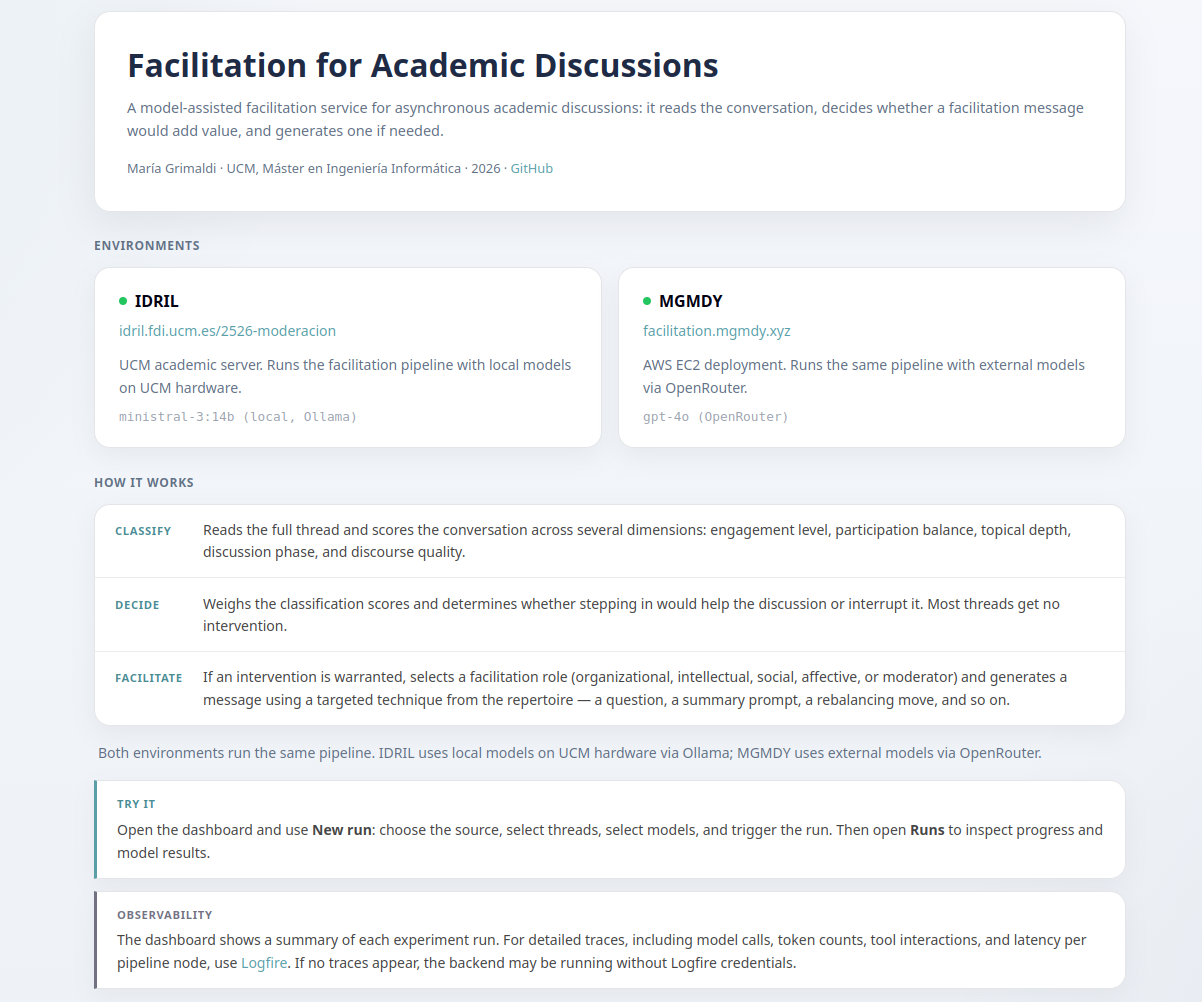
\includegraphics[width=0.85\textwidth]{figures/landing-page-tfm}
\caption{Página de entrada al proyecto, con los dos entornos experimentales y un resumen del funcionamiento.}
\label{fig:landing-page}
\end{figure}

\FloatBarrier
Dentro del panel, la navegación se concentra en dos opciones: \emph{New run}, para crear una ejecución, y \emph{Runs}, para consultar las anteriores. \emph{New run} presenta cuatro bloques desplegables (figura~\ref{fig:new-run-threads}). Primero se elige entre \emph{Sample data}, los hilos incluidos con el proyecto, y \emph{Live course}, que carga una instantánea de un curso. Después se revisan los hilos disponibles y se marcan los que formarán parte de la ejecución. Cada hilo puede abrirse antes de seleccionarlo.

\begin{figure}[htbp]
\centering
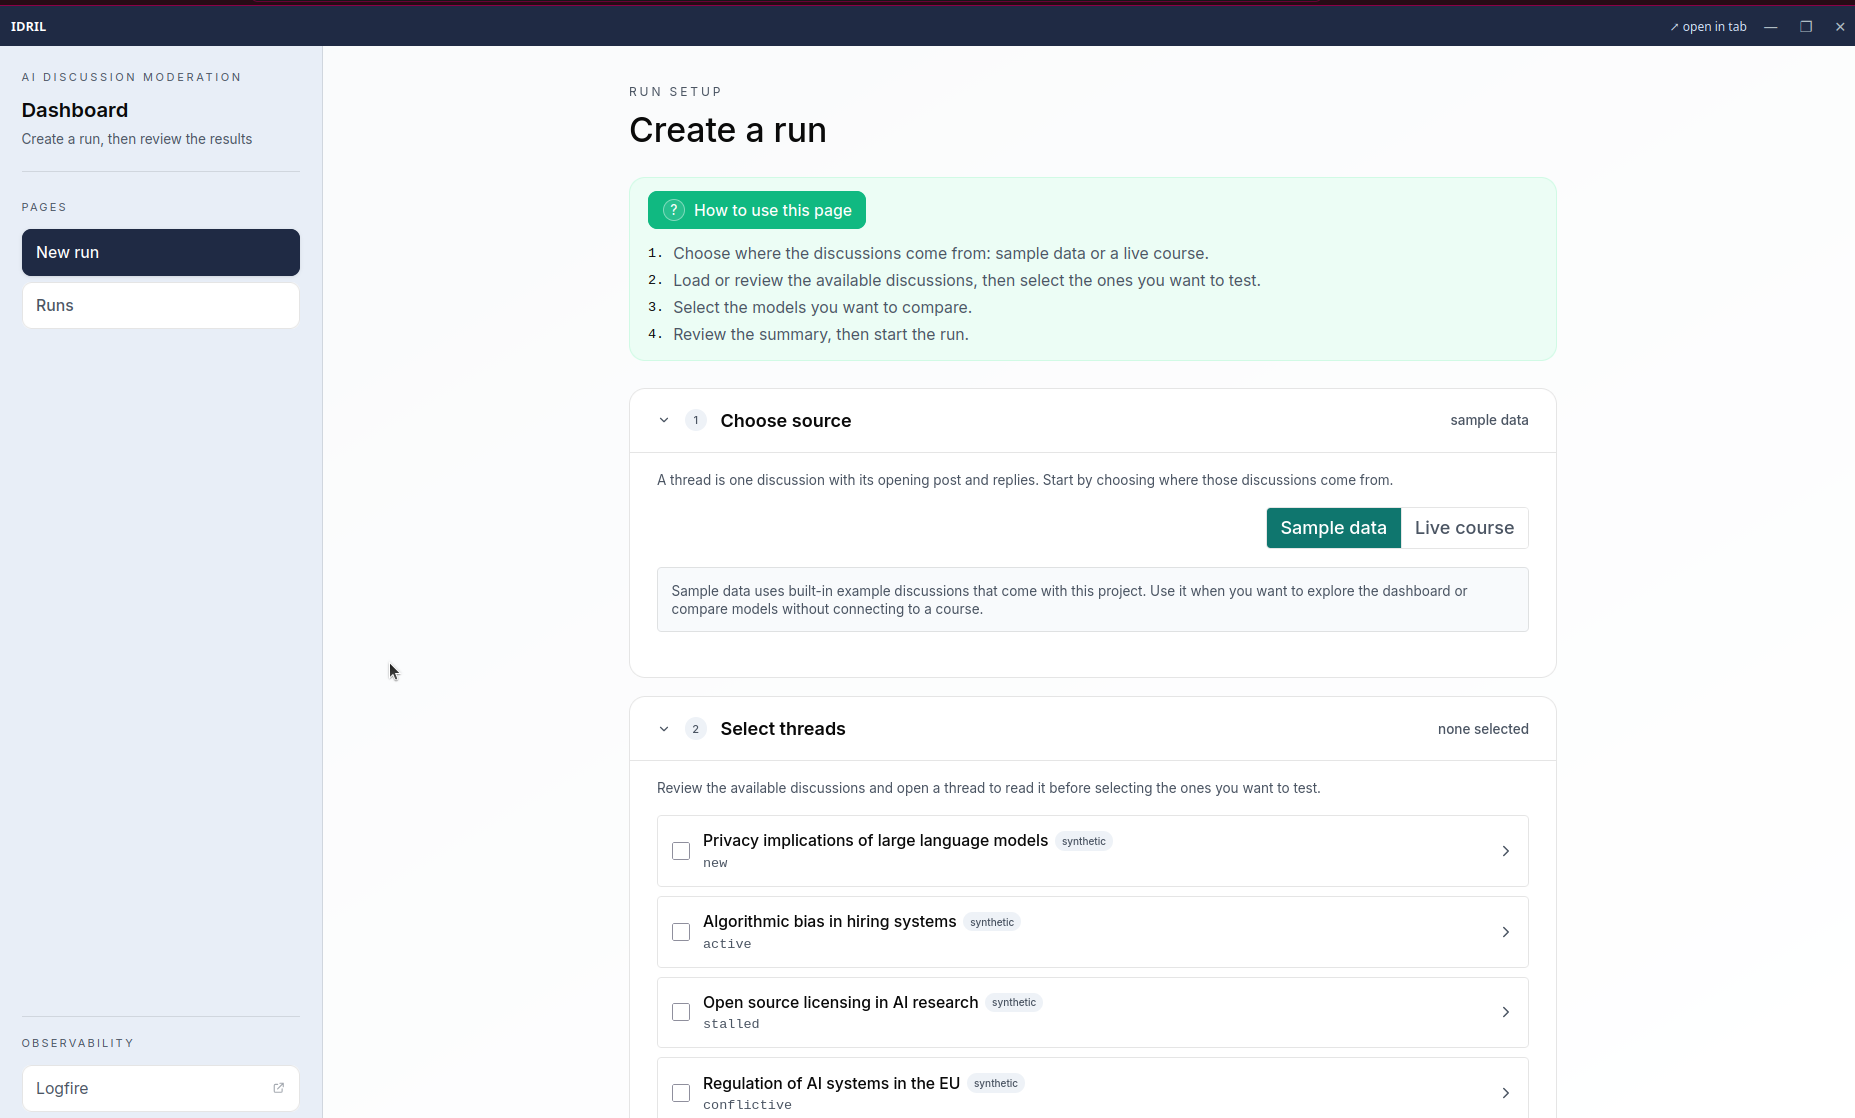
\includegraphics[width=0.95\textwidth]{figures/dashboard-new-run-threads-latest}
\caption{Primeros pasos de una ejecución: elección de la fuente y selección de hilos.}
\label{fig:new-run-threads}
\end{figure}

\FloatBarrier
El tercer bloque selecciona los modelos que se compararán y el cuarto resume el número de hilos, modelos y comparaciones antes de iniciar la ejecución (figura~\ref{fig:new-run-models}). El tamaño del experimento es el producto de los hilos y modelos seleccionados. Al iniciarlo, sus resultados se guardan para inspección.

\begin{figure}[htbp]
\centering
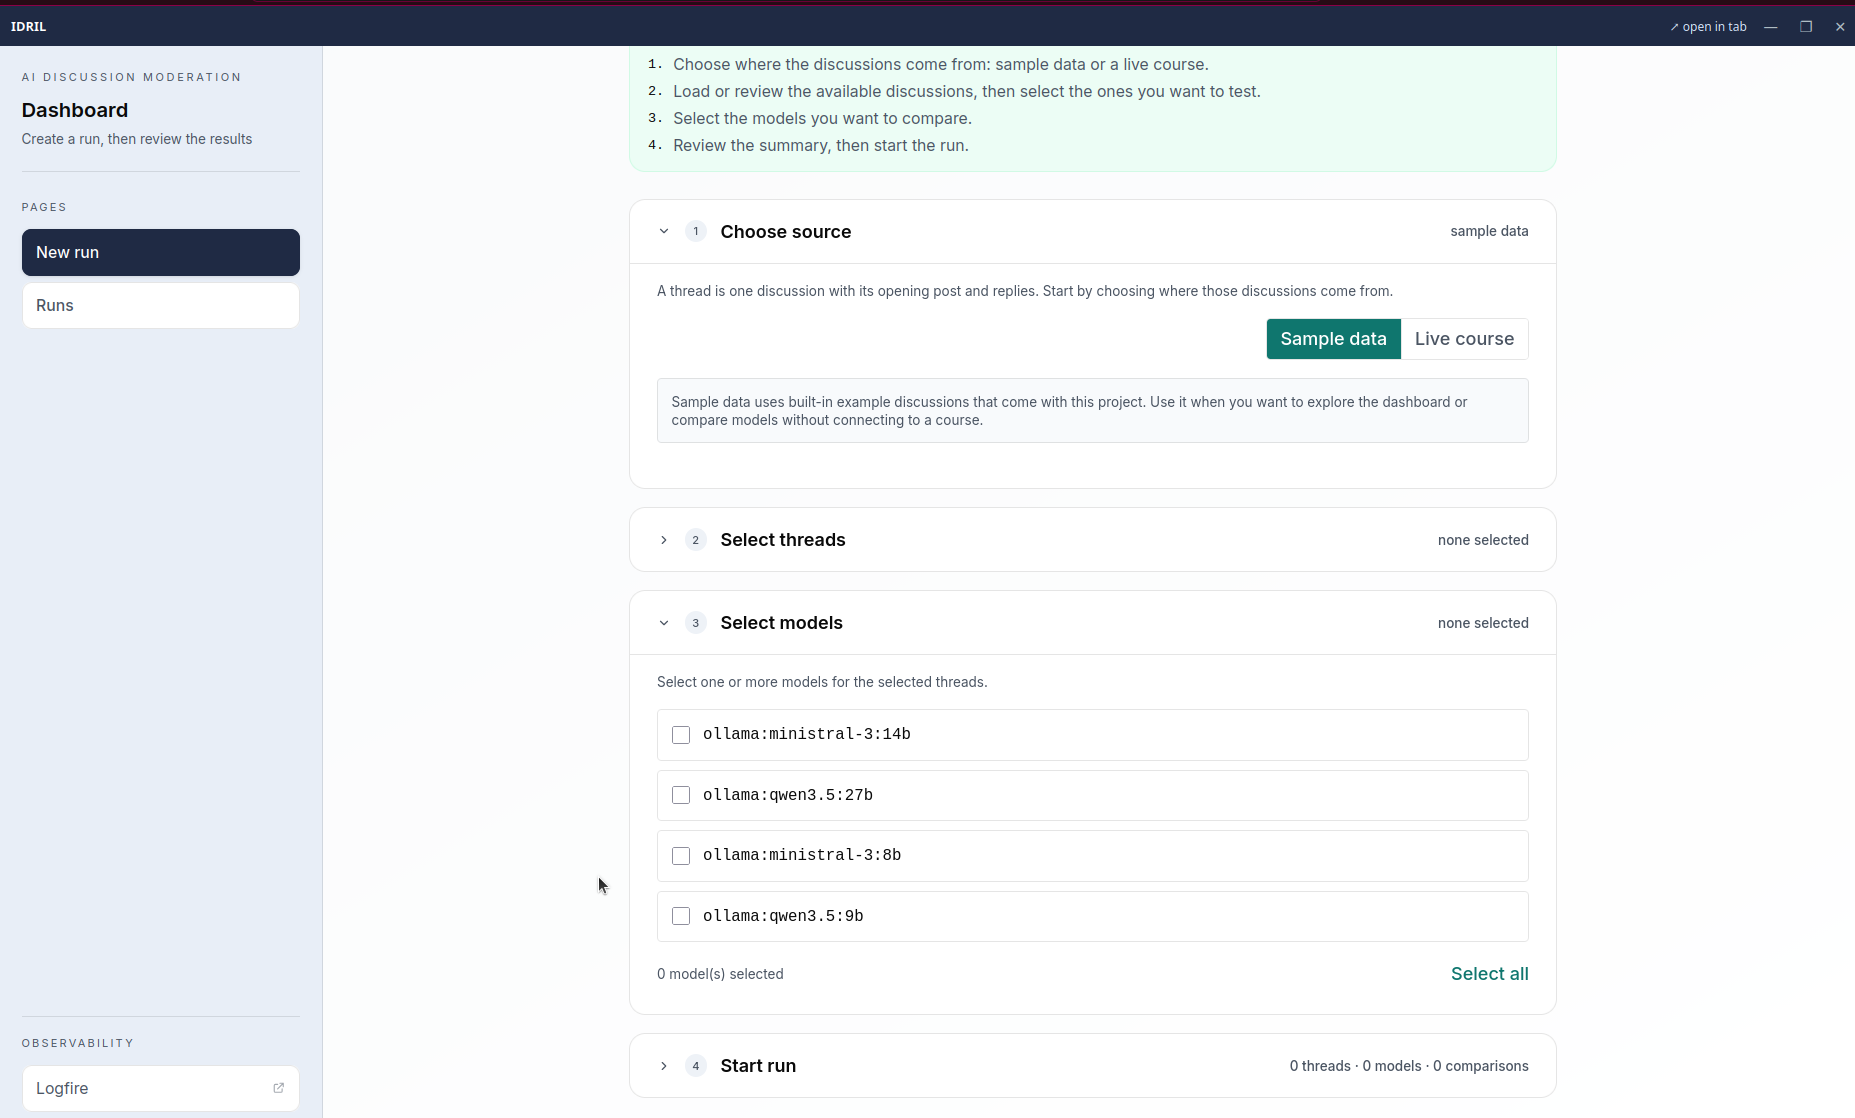
\includegraphics[width=0.95\textwidth]{figures/dashboard-new-run-models-latest}
\caption{Selección de modelos y resumen del número de comparaciones antes de iniciar la ejecución.}
\label{fig:new-run-models}
\end{figure}

\FloatBarrier
La opción \emph{Runs} abre el historial (figura~\ref{fig:run-history}). Cada fila muestra el nombre y la fecha de la ejecución, cuántas comparaciones terminaron y su estado. Una ejecución puede aparecer terminada, cancelada o interrumpida por el reinicio del servicio. Al abrirla, el panel muestra primero un resumen con el número de modelos, evaluaciones ejecutadas y errores. Debajo aparece la comparación por modelo, con ejecuciones completadas, velocidad media, errores y un enlace al detalle (figura~\ref{fig:run-overview}). También se puede preparar una nueva ejecución con la misma configuración mediante \emph{Retry run}.

\begin{figure}[htbp]
\centering
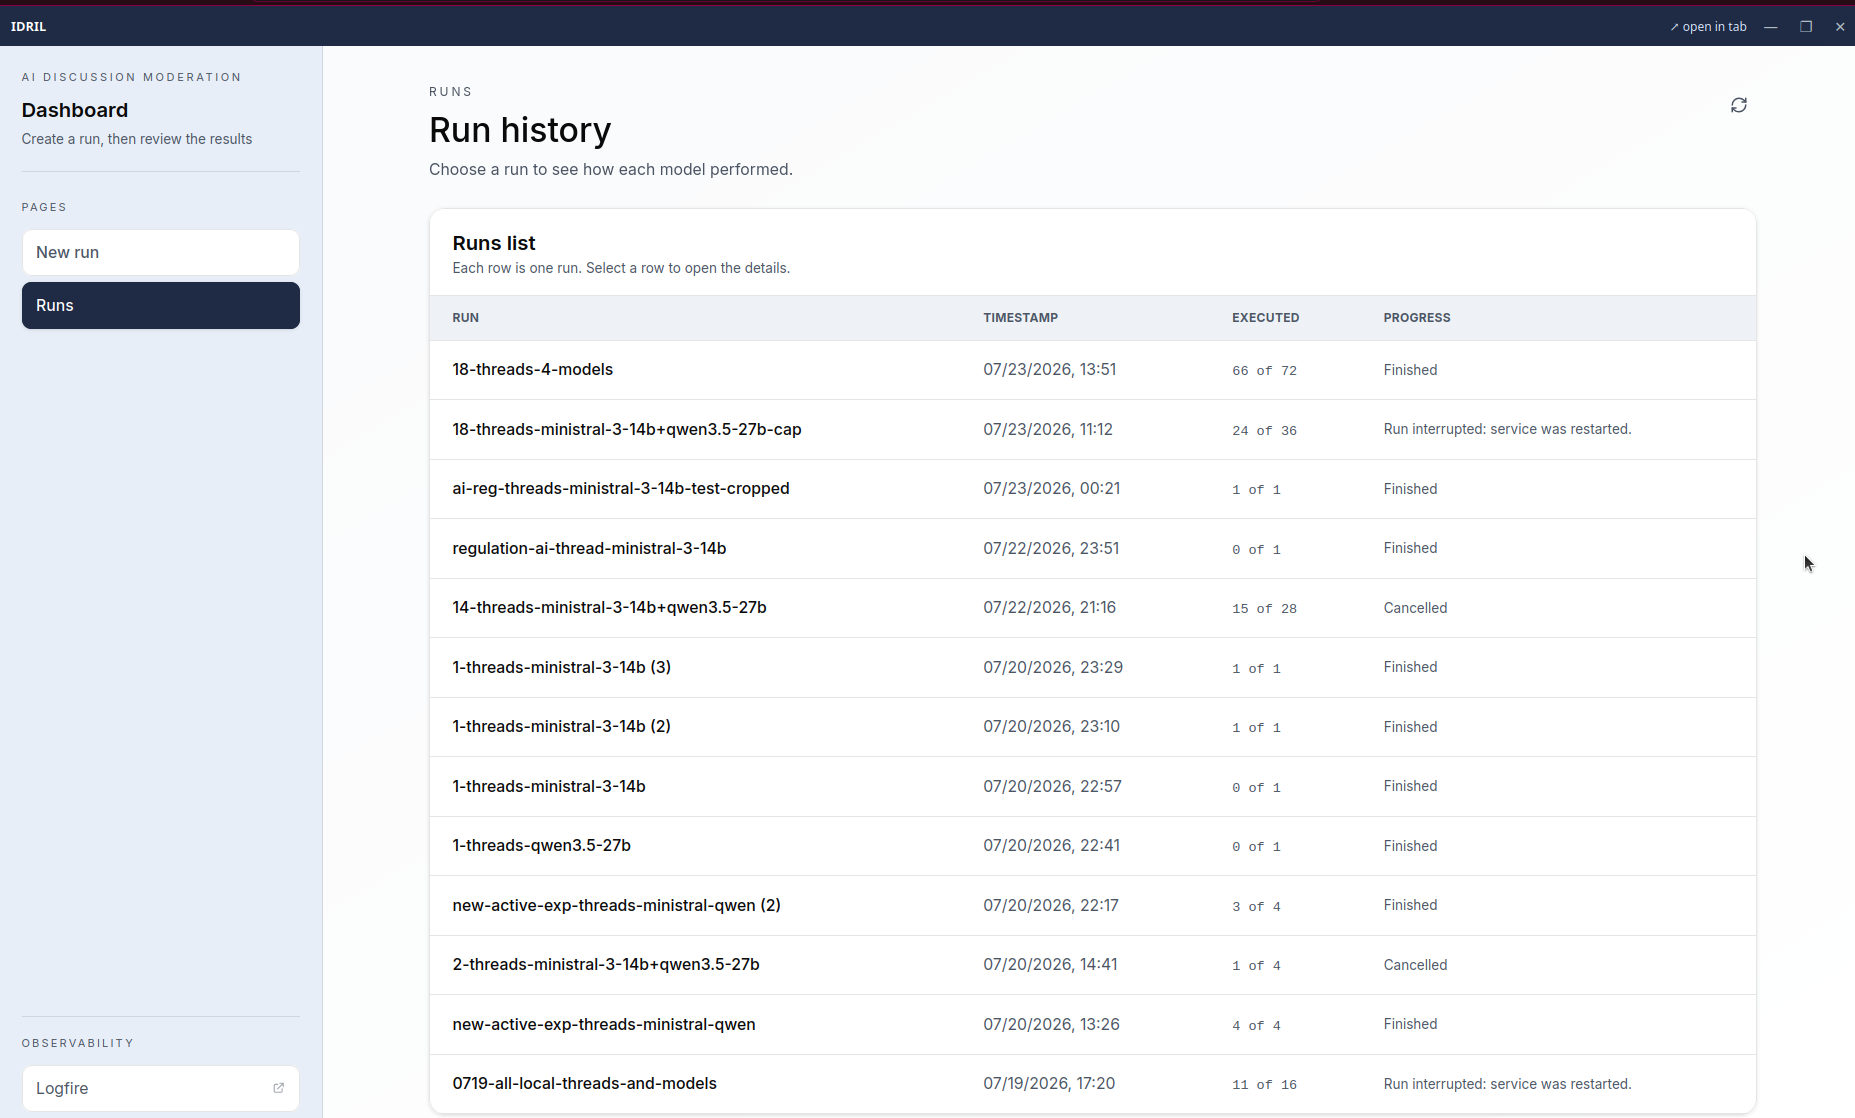
\includegraphics[width=0.95\textwidth]{figures/dashboard-run-history-latest}
\caption{Historial de ejecuciones con progreso y estado final.}
\label{fig:run-history}
\end{figure}

\begin{figure}[htbp]
\centering
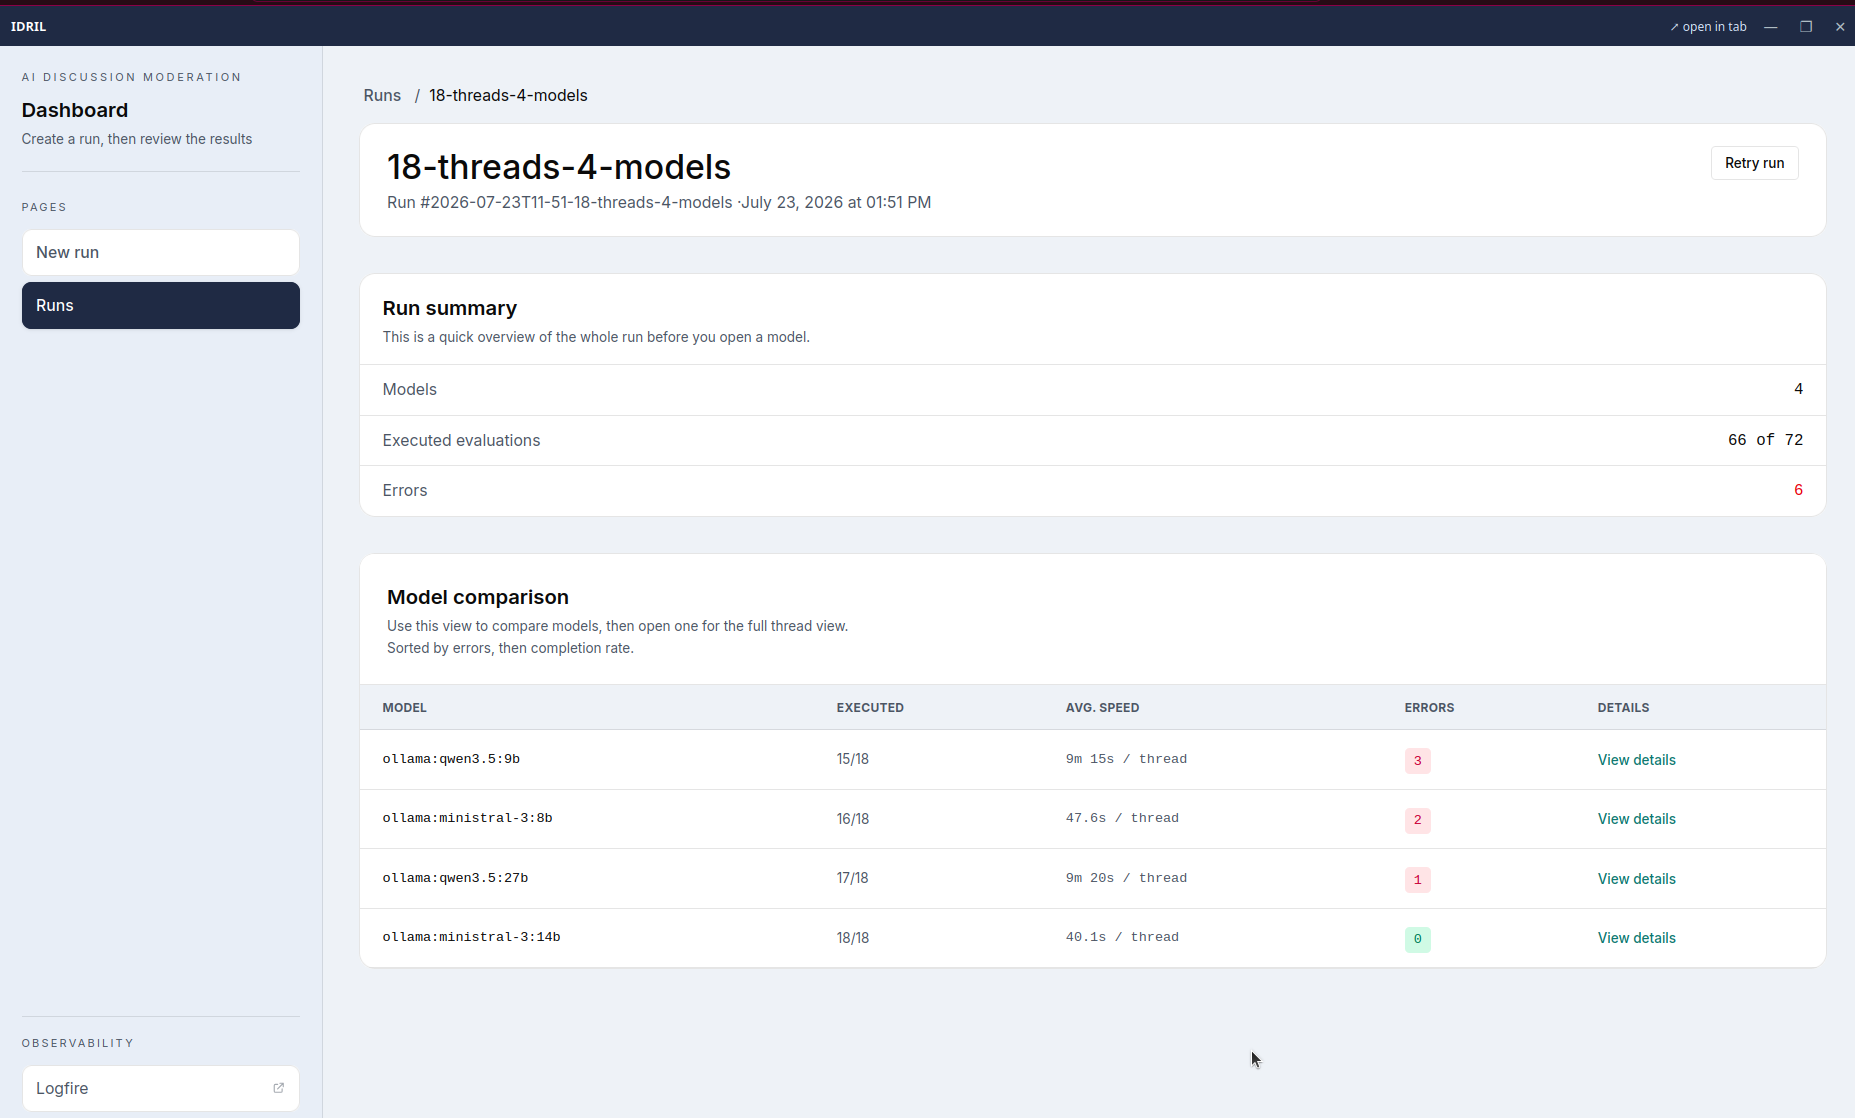
\includegraphics[width=0.95\textwidth]{figures/dashboard-run-overview-latest}
\caption{Resumen de una ejecución y comparación de completitud, velocidad y errores por modelo.}
\label{fig:run-overview}
\end{figure}

\FloatBarrier
Al abrir un modelo, el panel indica la fuente de los hilos, resume su completitud, número de acciones sugeridas, errores y velocidad media, y presenta la lista de hilos revisados (figura~\ref{fig:model-detail}). Cada fila anticipa la predicción y si el modelo propone intervenir. Estas etiquetas son resultados del modelo; cuando existe una clasificación local de referencia, la interfaz la presenta solo como orientación y no como verdad de referencia.

\begin{figure}[htbp]
\centering
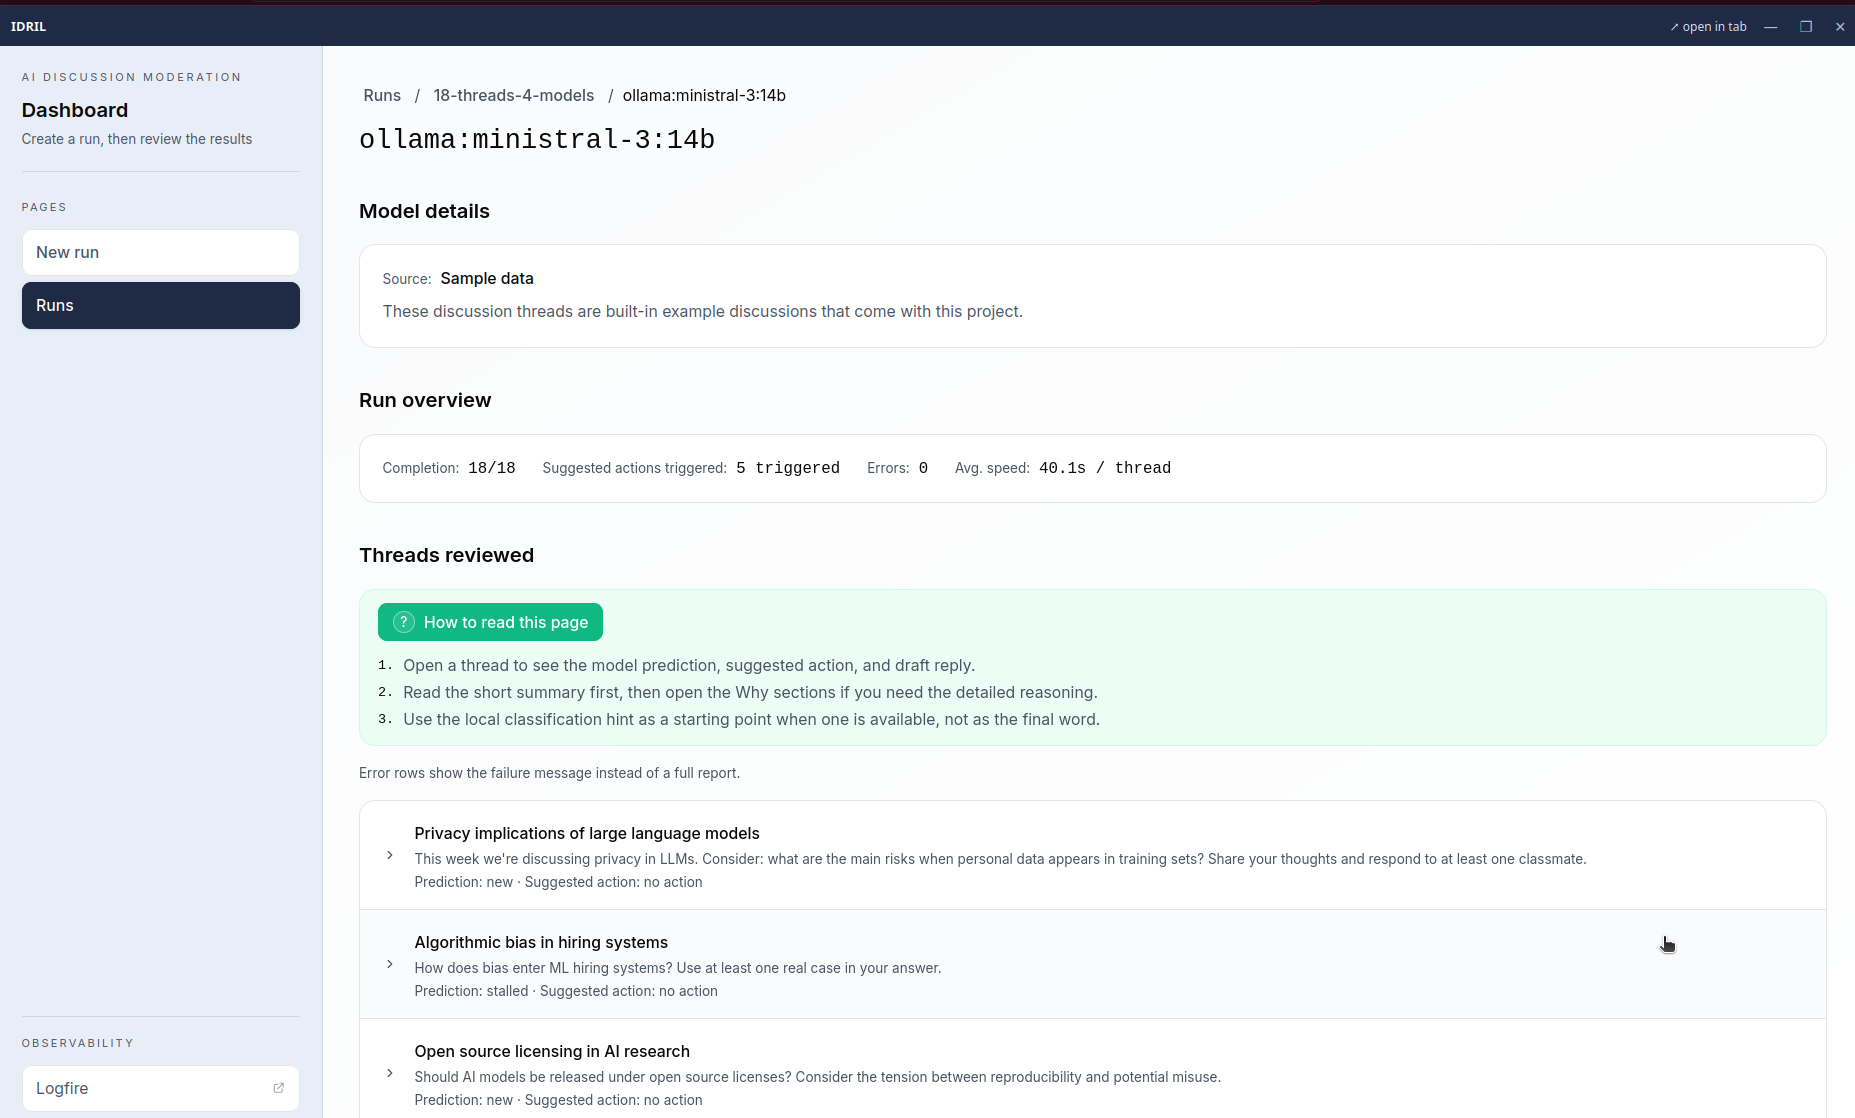
\includegraphics[width=0.95\textwidth]{figures/dashboard-model-detail-latest}
\caption{Detalle de un modelo dentro de una ejecución y lista de hilos revisados.}
\label{fig:model-detail}
\end{figure}

La vista final de cada hilo, con la discusión, la predicción, la acción sugerida y la respuesta candidata, se muestra en la figura~\ref{fig:thread-analysis}.


\backmatter

% (Sección de contribuciones eliminada)

\printbibliography[heading=bibintoc]

\end{document}
